% Presentación de la sustentación (Beamer, 16:9). Compilar con XeLaTeX desde esta carpeta:
%   xelatex presentacion.tex                                                   -> presentacion.pdf
%   xelatex -jobname=presentacion_notas "\def\connotas{}% Presentación de la sustentación (Beamer, 16:9). Compilar con XeLaTeX desde esta carpeta:
%   xelatex presentacion.tex                                                   -> presentacion.pdf
%   xelatex -jobname=presentacion_notas "\def\connotas{}% Presentación de la sustentación (Beamer, 16:9). Compilar con XeLaTeX desde esta carpeta:
%   xelatex presentacion.tex                                                   -> presentacion.pdf
%   xelatex -jobname=presentacion_notas "\def\connotas{}% Presentación de la sustentación (Beamer, 16:9). Compilar con XeLaTeX desde esta carpeta:
%   xelatex presentacion.tex                                                   -> presentacion.pdf
%   xelatex -jobname=presentacion_notas "\def\connotas{}\input{presentacion}"  -> notas del orador
% Las cifras salen de ../articulo/tablas/cifras.tex (analisis/analisis_resultados.py) y las
% figuras de ../analisis/figuras/diapositivas (analisis/figuras_diapositivas.py).
\ifdefined\connotas
  \documentclass[aspectratio=169,11pt,notes=only]{beamer}
\else
  \documentclass[aspectratio=169,11pt]{beamer}
\fi

\usepackage{fontspec}
\usepackage[spanish,es-noshorthands]{babel}
\usepackage{booktabs}
\usepackage{tikz}
\usepackage{listings}
\usetikzlibrary{arrows.meta,positioning,calc,fit,backgrounds}

% ------------------------------------------------------------------ tipografía
\setsansfont{IBMPlexSans}[Path=../analisis/fuentes/, Extension=.ttf, UprightFont=*-Regular,
  BoldFont=*-SemiBold, ItalicFont=*-Regular, ItalicFeatures={FakeSlant=0.18}]
\newfontfamily\plexmedia{IBMPlexSans-Medium}[Path=../analisis/fuentes/, Extension=.ttf]
\usefonttheme{professionalfonts}
\usefonttheme[onlymath]{serif}
\hyphenpenalty=10000
\exhyphenpenalty=10000

% ------------------------------------------------------------------ colores
% terracota = publicidad (con campaña), azul = imitación (sin campaña), igual que en el modelo y las figuras
\definecolor{papel}{HTML}{FBFAF6}
\definecolor{tinta}{HTML}{1F2933}
\definecolor{secundario}{HTML}{5E6670}
\definecolor{tenue}{HTML}{8C8A85}
\definecolor{borde}{HTML}{B9B4AA}
\definecolor{claro}{HTML}{F1EEE7}
\definecolor{azul}{HTML}{1E66A8}
\definecolor{azulclaro}{HTML}{8DB3D6}
\definecolor{azulfondo}{HTML}{E4EDF6}
\definecolor{terracota}{HTML}{C2502A}
\definecolor{terracotafondo}{HTML}{F7E6DE}

\setbeamercolor{background canvas}{bg=papel}
\setbeamercolor{normal text}{fg=tinta}
\setbeamercolor{structure}{fg=azul}
\setbeamercolor{frametitle}{fg=tinta}
\setbeamercolor{alerted text}{fg=terracota}
\setbeamercolor{item}{fg=terracota}
\setbeamercolor{enumerate item}{fg=terracota}

% ------------------------------------------------------------------ plantillas
\setbeamertemplate{navigation symbols}{}
\setbeamersize{text margin left=13mm, text margin right=13mm}
\setbeamerfont{frametitle}{size=\Large}
\newcommand{\seccion}{}
\setbeamertemplate{frametitle}{%
  \vskip6mm%
  {\scriptsize\addfontfeatures{LetterSpace=12}\color{terracota}\MakeUppercase{\seccion}}\par\vskip1mm%
  {\usebeamerfont{frametitle}\plexmedia\color{tinta}\insertframetitle\par}\vskip0.5mm}
\setbeamertemplate{footline}{%
  \hbox to \paperwidth{\hskip13mm{\fontsize{6}{7}\selectfont\color{tenue}Delgado · Monroy · Baquero\quad Universidad de los Llanos}%
  \hfill{\fontsize{6}{7}\selectfont\color{tenue}\insertframenumber\,/\,\inserttotalframenumber}\hskip13mm}\vskip4mm}
\setbeamertemplate{itemize item}{\raisebox{0.3ex}{\color{terracota}\rule{0.8ex}{0.8ex}}}
\setbeamertemplate{enumerate item}{\color{terracota}\plexmedia\insertenumlabel.}
\setbeamertemplate{itemize/enumerate body begin}{\raggedright}
\setlength{\leftmargini}{1.3em}
\setbeamertemplate{note page}{\vskip5mm\hskip6mm\begin{minipage}[t]{0.42\paperwidth}\vskip0pt\insertslideintonotes{0.4}\end{minipage}%
  \hskip4mm\begin{minipage}[t]{0.4\paperwidth}\vskip0pt\raggedright\footnotesize
  {\scriptsize\color{terracota}DIAPOSITIVA \insertframenumber}\par\vskip2mm\insertnote\end{minipage}}

\lstset{basicstyle=\ttfamily\fontsize{7.2}{8.6}\selectfont\color{tinta}, keywordstyle=\color{azul}, columns=fullflexible,
  keepspaces=true, frame=none, aboveskip=0pt, belowskip=0pt,
  morekeywords={to,end,ask,let,set,if,with,count,any?,random-float,turtles,link-neighbors,not}}

% ------------------------------------------------------------------ utilidades
\newcommand{\cifra}[2]{% número grande + leyenda
  \begin{minipage}[t]{\linewidth}\raggedright{\plexmedia\fontsize{24}{26}\selectfont\color{azul}#1\par}\vskip1mm
  {\small\color{secundario}#2\par}\end{minipage}}
\newcommand{\nota}[1]{{\raggedright\footnotesize\color{secundario}#1\par}}
\newcommand{\fuente}[1]{\par\vfill{\fontsize{6}{7}\selectfont\color{tenue}#1}\par\vskip1mm}
\newcommand{\referencia}[1]{\par\hangindent=1.4em\hangafter=1 #1\par}

\input{../articulo/tablas/cifras}
\graphicspath{{figuras/}{../analisis/figuras/diapositivas/}{../articulo/figuras/}}

\begin{document}

% =================================================================== 1. portada
{\setbeamertemplate{footline}{}
\begin{frame}[plain]
  \begin{columns}[c,totalwidth=\textwidth]
    \begin{column}{0.62\textwidth}
      \raggedright
      {\scriptsize\addfontfeatures{LetterSpace=12}\color{terracota}PROYECTO 14 · SIMULACIÓN COMPUTACIONAL}\par\vskip5mm
      {\plexmedia\fontsize{21}{26}\selectfont\color{tinta}Publicidad y redes sociales en la difusión de innovaciones\par}\vskip3mm
      {\color{secundario}Un modelo basado en agentes de la PS5 y del lanzamiento de GTA\,6\par}\vskip8mm
      {\small Jesus Gregorio Delgado\\ David Andres Monroy Aguiar\\ Duvan Felipe Baquero Cerquera\par}\vskip5mm
      {\scriptsize\color{tenue}Ingeniería de Sistemas · Universidad de los Llanos\\ 17 de noviembre de 2026\par}
    \end{column}
    \begin{column}{0.36\textwidth}
      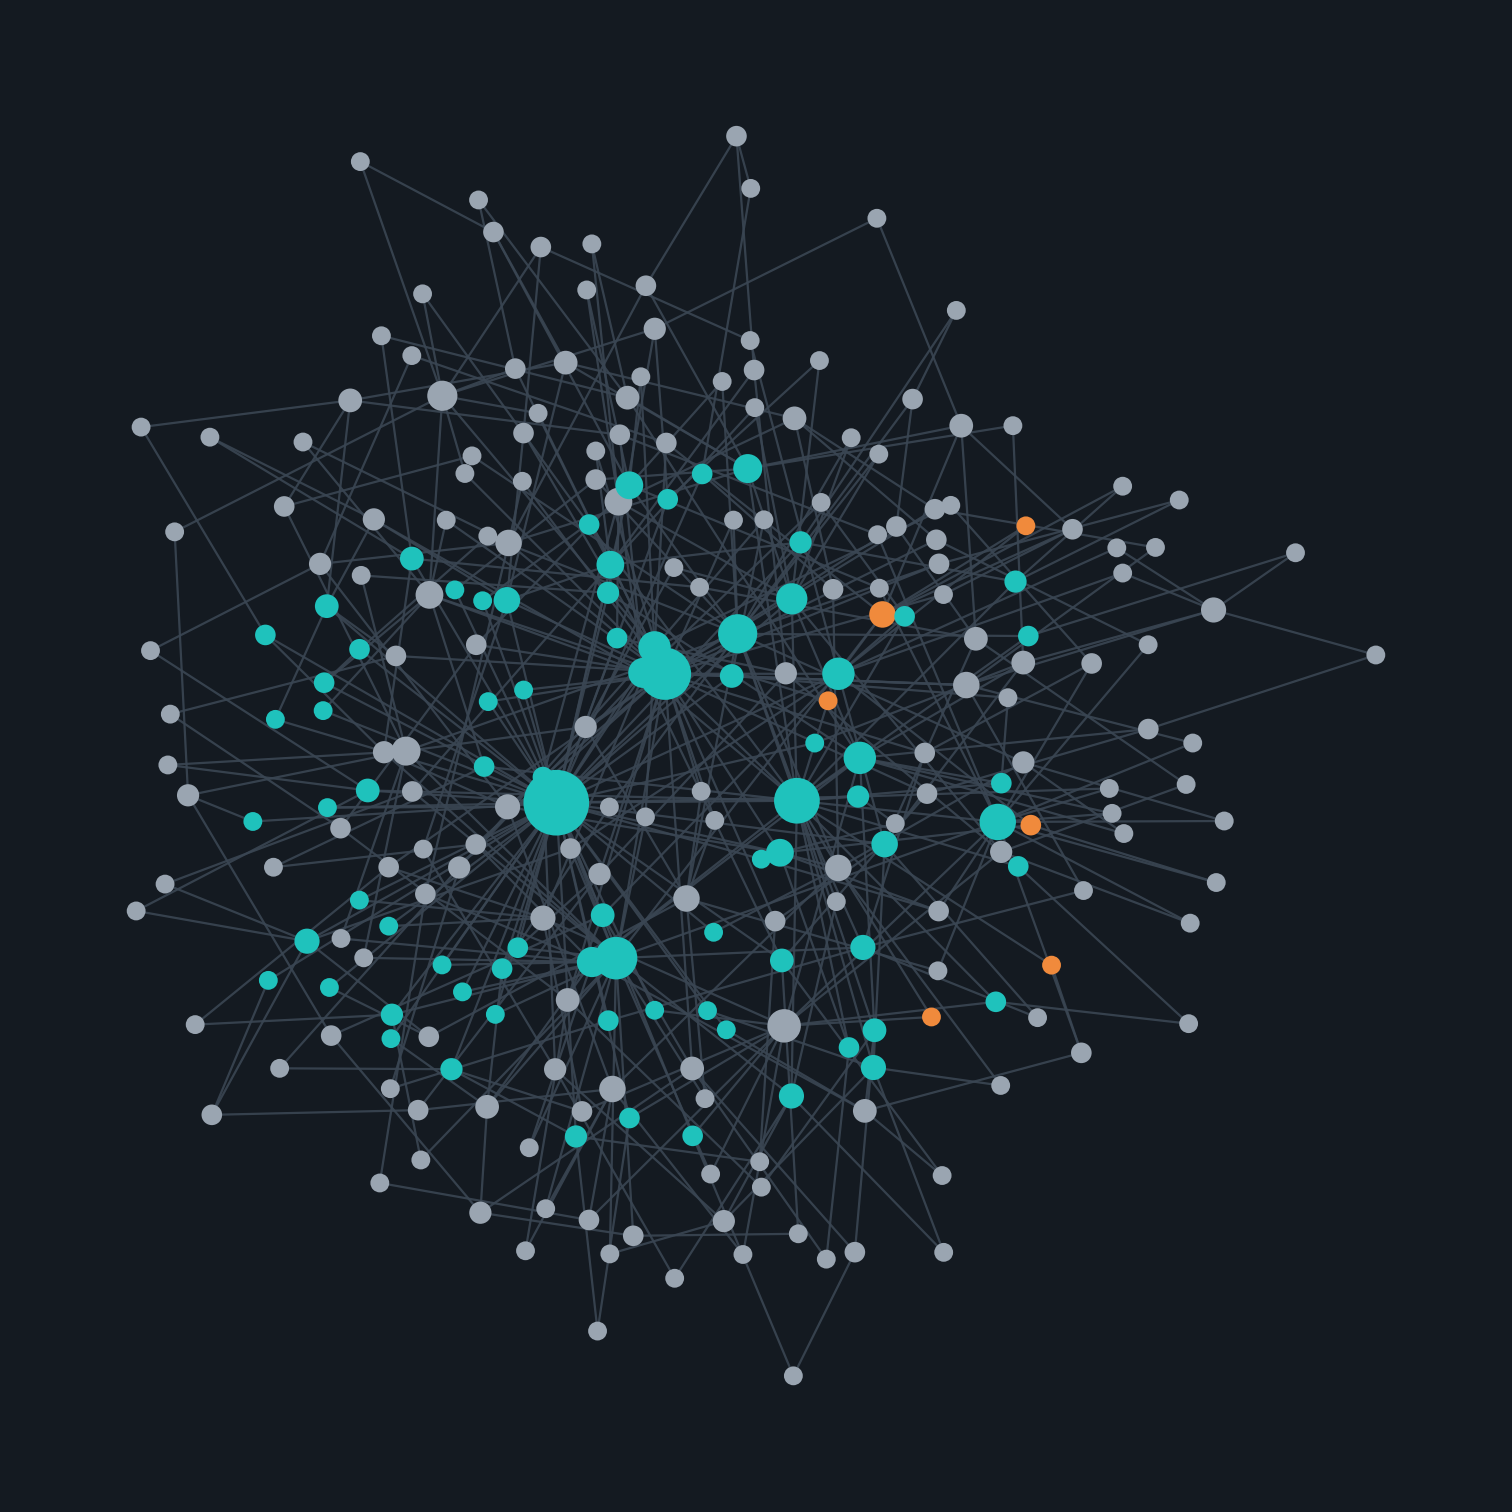
\includegraphics[width=\linewidth]{portada_red.png}
    \end{column}
  \end{columns}
\end{frame}
}
\note{\textbf{Jesus (0:40).} Buenos días. Somos Jesus, David y Duvan. Nuestro proyecto simula cómo se difunde un producto nuevo cuando cada persona decide influida por la publicidad y por sus contactos. Lo aplicamos a dos casos de actualidad: la PS5, una tecnología, y GTA\,6, un videojuego que sale este jueves. Lo construimos en NetLogo, lo calibramos con datos reales y lo usamos para comparar escenarios que no se pueden observar.}

% =================================================================== 2. motivación
\renewcommand{\seccion}{Motivación}
\begin{frame}{Dos lanzamientos, dos maneras de difundirse}
  \vskip4mm
  \begin{columns}[t,totalwidth=\textwidth]
    \begin{column}{0.31\textwidth}\cifra{\cifraPsUnidadesFin\,M}{PS5 vendidas de noviembre de 2020 a septiembre de 2026}\end{column}
    \begin{column}{0.31\textwidth}\cifra{19 nov.}{sale GTA\,6, solo para consolas de esta generación}\end{column}
    \begin{column}{0.31\textwidth}\cifra{90\,M}{vistas del primer tráiler de GTA\,6 en 24 horas}\end{column}
  \end{columns}
  \vskip8mm
  \begin{itemize}
    \item Bass: un producto se difunde por \textcolor{terracota}{publicidad} (externa) e \textcolor{azul}{imitación} (voz a voz).
    \item La PS5 crece por imitación; un gran estreno vende casi todo al salir.
  \end{itemize}
  \fuente{Sony Interactive Entertainment, Business Data \& Sales; Guinness World Records (2023).}
\end{frame}
\note{\textbf{Jesus (0:45).} La PS5 ya pasa de \cifraPsUnidadesFin\ millones de unidades, y sobre esa base sale GTA\,6 el 19 de noviembre, después de una campaña que rompió récords: 90 millones de vistas del primer tráiler en un día. Bass explicó la difusión con dos fuerzas: la publicidad, que llega a todos, y la imitación, que depende de cuántos ya adoptaron. Cuando manda la imitación sale la curva en S, como en la PS5; cuando manda la publicidad, las ventas se concentran en el lanzamiento.}

% =================================================================== 3. problema
\renewcommand{\seccion}{Problema}
\begin{frame}{El modelo agregado no ve la red social}
  \vskip2mm
  \begin{columns}[c,totalwidth=\textwidth]
    \begin{column}{0.52\textwidth}
      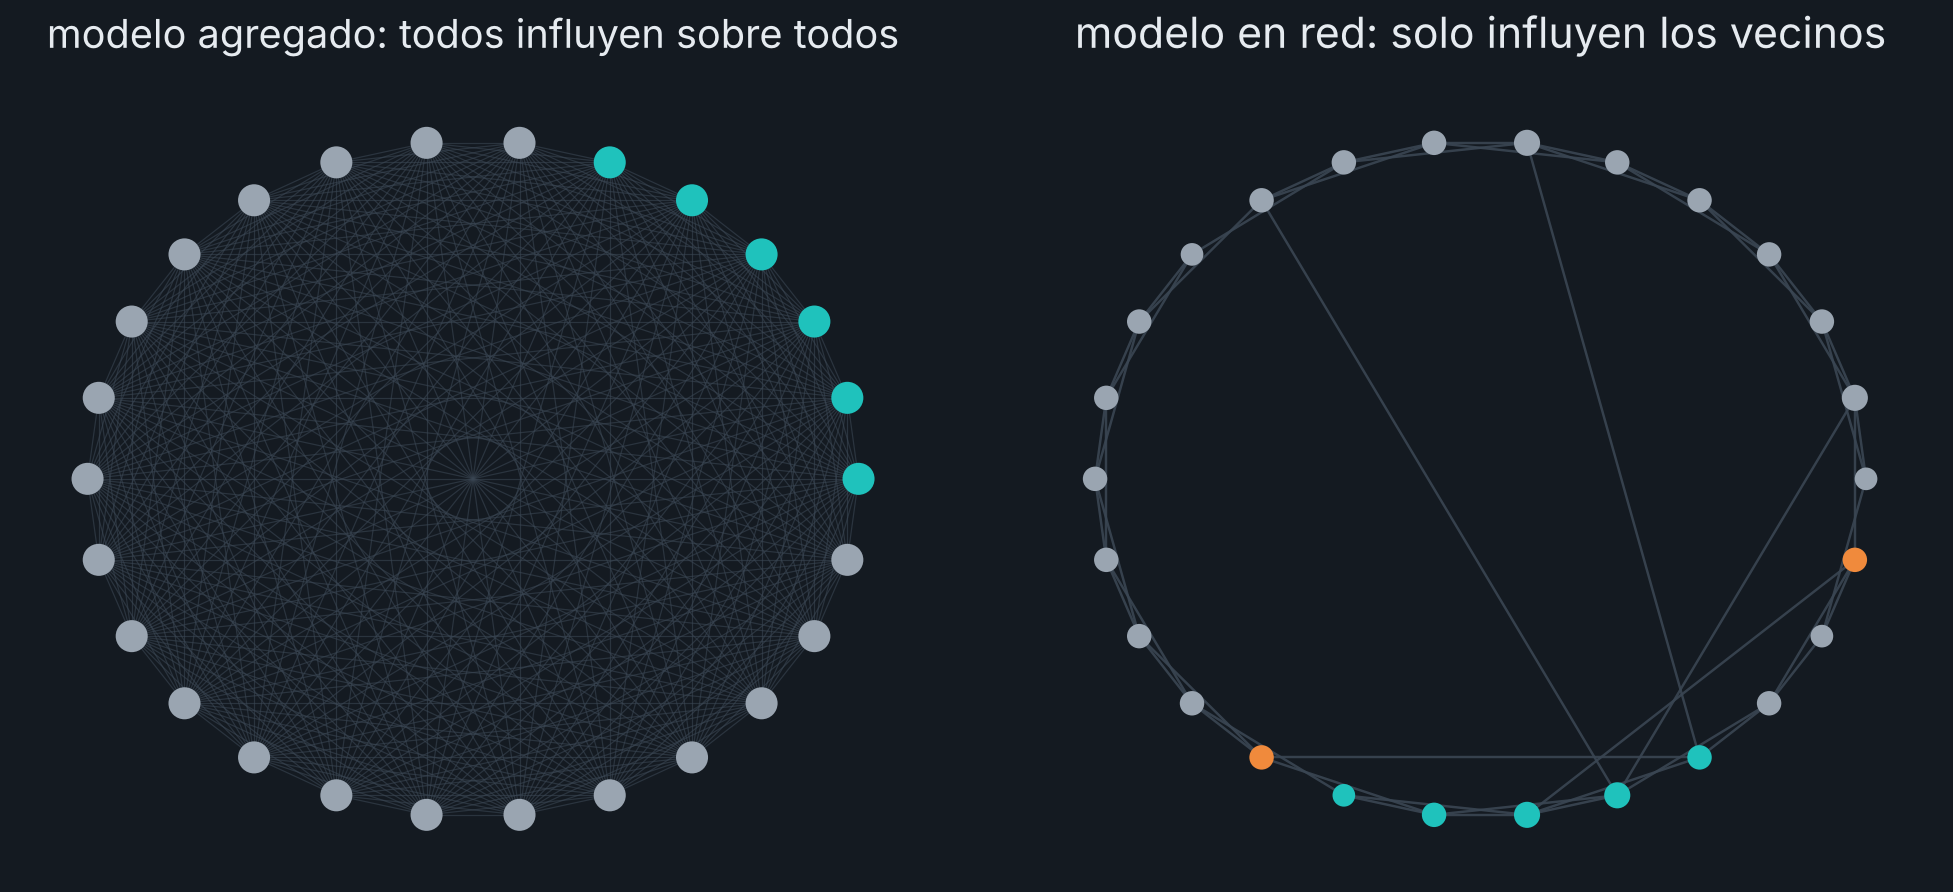
\includegraphics[width=\linewidth]{mezcla_vs_red.png}
    \end{column}
    \begin{column}{0.44\textwidth}
      \raggedright
      Bass: todos influyen sobre todos. En la realidad, solo los contactos.\par\vskip3mm
      \begin{itemize}
        \item ¿Qué pasa sin publicidad?
        \item ¿Importa la densidad o la forma de la red?
        \item ¿Cuánto se pierde con una campaña corta?
        \item ¿Responden igual una consola y un videojuego?
      \end{itemize}
    \end{column}
  \end{columns}
\end{frame}
\note{\textbf{Jesus (0:50).} El modelo de Bass describe bien las curvas agregadas, pero supone que todos influyen sobre todos, como en la red de la izquierda. En la vida real la influencia viaja por una red concreta, como la de la derecha. Eso deja cuatro preguntas sin responder: qué pasa sin publicidad, si importa la estructura de la red, cuánto se pierde con una campaña corta y si una consola y un videojuego responden igual.}

% =================================================================== 4. justificación
\renewcommand{\seccion}{Justificación}
\begin{frame}{Simular permite probar lo que no se puede observar}
  \vskip5mm
  \begin{columns}[t,totalwidth=\textwidth]
    \begin{column}{0.3\textwidth}
      {\plexmedia\color{azul}Individuos y red}\par\vskip2mm
      \nota{Cada persona es un agente con sus contactos y una regla de decisión.}
    \end{column}
    \begin{column}{0.3\textwidth}
      {\plexmedia\color{azul}Contrafactuales}\par\vskip2mm
      \nota{Lanzar sin publicidad, cambiar la red o acortar la campaña: imposible de observar en la realidad.}
    \end{column}
    \begin{column}{0.3\textwidth}
      {\plexmedia\color{azul}Datos reales}\par\vskip2mm
      \nota{PS5: calibrada y evaluada con ventas oficiales. GTA\,6, sin ventas aún: por analogía con GTA\,V.}
    \end{column}
  \end{columns}
  \vskip10mm
  \nota{NetLogo: libre, el modelo completo en un archivo y BehaviorSpace para repetir cada escenario 30 veces.}
\end{frame}
\note{\textbf{Jesus (0:50).} La simulación basada en agentes responde esas preguntas porque representa a cada persona y sus contactos, y permite correr escenarios que no se pueden observar, como lanzar sin publicidad. Para que no fuera un ejercicio solo cualitativo, la PS5 se calibró con las ventas oficiales de Sony y se evaluó con datos que no usamos para ajustar. GTA\,6 todavía no tiene ventas, así que sus parámetros salen por analogía con GTA\,V, que es la práctica estándar antes de un lanzamiento.}

% =================================================================== 5. objetivos
\renewcommand{\seccion}{Objetivos}
\begin{frame}{Qué nos propusimos}
  \vskip2mm
  {\plexmedia General.} Medir el efecto de la publicidad y de la red sobre la adopción final, en la PS5 y en GTA\,6.\par\vskip5mm
  {\plexmedia Específicos}\par\vskip1mm
  \begin{enumerate}
    \item Implementar en NetLogo el modelo de Bass en red, con tres tipos de red.
    \item Calibrar con la PS5 (entrenamiento, validación, prueba) y parametrizar GTA\,6 por analogía.
    \item Evaluar con 30 réplicas publicidad, densidad, topología y duración.
    \item Verificar con una reimplementación en Python.
  \end{enumerate}
\end{frame}
\note{\textbf{Jesus (0:40).} El objetivo general es medir el efecto de la publicidad y de la red sobre la adopción final, en la PS5 y en GTA\,6. Los específicos: implementarlo en NetLogo con tres tipos de red, calibrarlo con partición entrenamiento-validación-prueba, evaluar los escenarios con réplicas y verificarlo con una reimplementación independiente en Python.}

% =================================================================== 6. modelo
\renewcommand{\seccion}{Metodología}
\begin{frame}{Cada mes, cada persona decide: publicidad y vecinos}
  \vskip4mm
  \begin{center}{\Large $P_i = 1 - (1 - \textcolor{terracota}{p\,a_t})\,(1 - \textcolor{azul}{q\,f_i})$}\end{center}
  \vskip5mm
  \begin{columns}[T,totalwidth=\textwidth]
    \begin{column}{0.46\textwidth}
      {\color{terracota}\plexmedia publicidad}\par\nota{$p$: probabilidad mensual de que la campaña convenza; $a_t=1$ mientras está activa.}\par\vskip3mm
      {\color{azul}\plexmedia imitación}\par\nota{$q$ por $f_i$, la fracción de vecinos que ya adoptó.}
    \end{column}
    \begin{column}{0.48\textwidth}
      \vskip-\topsep
      {\small\begin{itemize}
        \item Adoptar es irreversible; todos deciden a la vez.
        \item Red completa = Bass: la diferencia es el efecto de la red.
        \item Redes aleatoria, mundo pequeño y libre de escala.
      \end{itemize}}
    \end{column}
  \end{columns}
\end{frame}
\note{\textbf{Jesus (1:00).} Cada agente es un nodo. Cada mes, quien no ha adoptado lo hace con esta probabilidad: la publicidad lo convence con probabilidad $p$ mientras la campaña esté activa, y sus vecinos con $q$ por la fracción de vecinos que ya adoptaron. Las decisiones se aplican todas a la vez al cerrar el mes y la adopción es irreversible. Si la red fuera completa, el modelo recuperaría la curva de Bass; la diferencia entre ambas es el efecto de la red. Usamos tres redes: aleatoria, mundo pequeño, con grupos cerrados, y libre de escala, con pocos nodos muy conectados. \emph{Le paso la palabra a David.}}

% =================================================================== 7. esquema
\begin{frame}{Del dato al escenario}
  \vskip2mm
  \begin{center}
  \begin{tikzpicture}[
    font=\small, text=tinta,
    caja/.style={draw=borde, line width=0.5pt, rounded corners=2pt, fill=white, align=center, inner sep=2pt,
                 minimum height=12mm, text width=21mm},
    etapa/.style={caja, fill=claro},
    flecha/.style={-{Latex[length=2mm]}, line width=0.8pt, draw=tinta},
    detalle/.style={font=\scriptsize, text=secundario}]
    \node[etapa] (d) at (0,0) {\plexmedia Datos\\[-1pt]{\scriptsize\color{secundario}Sony, Take-Two}};
    \node[etapa] (c) at (2.78,0) {\plexmedia Calibración\\[-1pt]{\scriptsize\color{secundario}Bass, analogía}};
    \node[etapa, fill=azulfondo, draw=azul, line width=0.8pt] (m) at (5.56,0) {\plexmedia Modelo\\[-1pt]{\scriptsize\color{secundario}NetLogo + nw}};
    \node[etapa] (e) at (8.34,0) {\plexmedia Escenarios\\[-1pt]{\scriptsize\color{secundario}BehaviorSpace}};
    \node[etapa] (a) at (11.12,0) {\plexmedia Análisis\\[-1pt]{\scriptsize\color{secundario}Python}};
    \draw[flecha] (d) -- (c); \draw[flecha] (c) -- (m);
    \draw[flecha] (m) -- (e); \draw[flecha] (e) -- (a);
    % interior del modelo
    \node[caja, fill=terracotafondo, draw=terracota, text width=27mm, minimum height=9mm] (camp) at (1.6,-2.5)
      {\plexmedia Campaña\\[-1pt]{\scriptsize $p\,a_t$}};
    \node[caja, fill=azulfondo, draw=azul, text width=27mm, minimum height=9mm] (red) at (1.6,-3.75)
      {\plexmedia Red social\\[-1pt]{\scriptsize $q\,f_i$}};
    \node[caja, fill=white, draw=azul, line width=0.8pt, text width=44mm, minimum height=21mm] (regla) at (6.3,-3.125)
      {\plexmedia Regla de adopción\\[4pt]$P_i = 1-(1-p\,a_t)(1-q\,f_i)$};
    \node[caja, text width=22mm, minimum height=12mm] (est) at (10.62,-3.125) {\plexmedia Estado\\[-1pt]{\scriptsize adopta y no vuelve atrás}};
    \draw[flecha, draw=terracota] (camp.east) -- (regla.west |- camp.east);
    \draw[flecha, draw=azul] (red.east) -- (regla.west |- red.east);
    \draw[flecha] (regla) -- (est);
    \begin{scope}[on background layer]
      \node[draw=azul, dashed, rounded corners=3pt, fit=(camp)(red)(regla)(est), inner sep=2.5mm] (int) {};
    \end{scope}
    \node[font=\scriptsize, text=azul, anchor=south west] at (int.north west) {cada mes, dentro del modelo};
    \draw[flecha, draw=azul, dashed] (m.south) -- (m.south |- int.north);
  \end{tikzpicture}
  \end{center}
\end{frame}
\note{\textbf{David (0:40).} Arriba el flujo: las ventas reales dan los parámetros, la PS5 por calibración de Bass y GTA\,6 por analogía con GTA\,V; NetLogo simula; BehaviorSpace corre los cuatro experimentos; Python calcula las medidas. Abajo, lo que pasa dentro del modelo cada mes: la campaña y la red alimentan la regla, que decide si cada persona adopta.}

% =================================================================== 8. implementación
\begin{frame}[fragile]{Implementación en NetLogo}
  \vskip1mm
  \begin{columns}[c,totalwidth=\textwidth]
    \begin{column}{0.47\textwidth}
      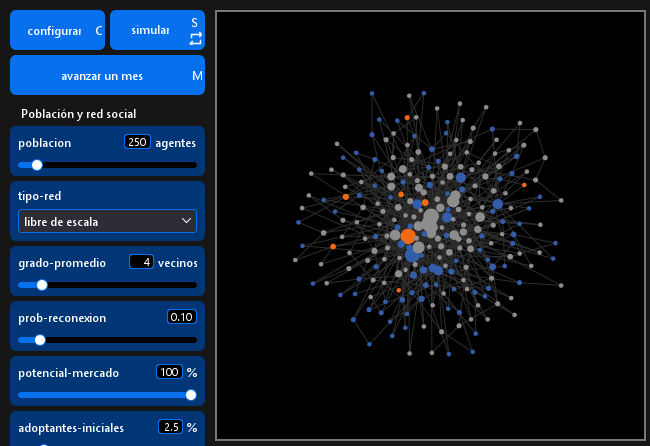
\includegraphics[width=\linewidth]{netlogo_ps5.png}\par\vskip1mm
      {\fontsize{6}{7}\selectfont\color{tenue}Interfaz del modelo (configuración de demostración: caso PS5, red libre de escala, mes 30).}
    \end{column}
    \begin{column}{0.5\textwidth}
\begin{lstlisting}
to decidir
  let p p-efectivo
  ask turtles with
      [susceptible? and not adoptante?] [
    let vecinos link-neighbors
    let f 0
    if any? vecinos [
      set f count vecinos with [adoptante?]
        / count vecinos ]
    let prob 1 - (1 - p) * (1 - q-imitacion * f)
    set decide-adoptar? random-float 1 < prob ]
end
\end{lstlisting}
      \vskip4mm
      \nota{\texttt{actualizar} aplica todas las decisiones a la vez. La extensión nw genera las redes; el selector de caso carga PS5, GTA\,6 o libre.}
    \end{column}
  \end{columns}
\end{frame}
\note{\textbf{David (0:50).} Esto es NetLogo con la extensión nw. A la izquierda, la interfaz con el caso PS5 en una red libre de escala: en azul los que ya adoptaron, en naranja los de este mes, y los nodos grandes son los más conectados. A la derecha, el procedimiento decidir: cada no adoptante cuenta qué fracción de sus vecinos ya adoptó y sortea su decisión con la fórmula. Un procedimiento aparte, actualizar, aplica todas las decisiones a la vez para que el orden de los agentes no afecte el resultado. El selector de caso carga los parámetros de la PS5 o de GTA\,6 con un clic.}

% =================================================================== 9. datos PS5
\renewcommand{\seccion}{Conjunto de datos}
\begin{frame}{La PS5: \cifraTrimestres\ trimestres de ventas oficiales de Sony}
  \begin{columns}[c,totalwidth=\textwidth]
    \begin{column}{0.6\textwidth}
      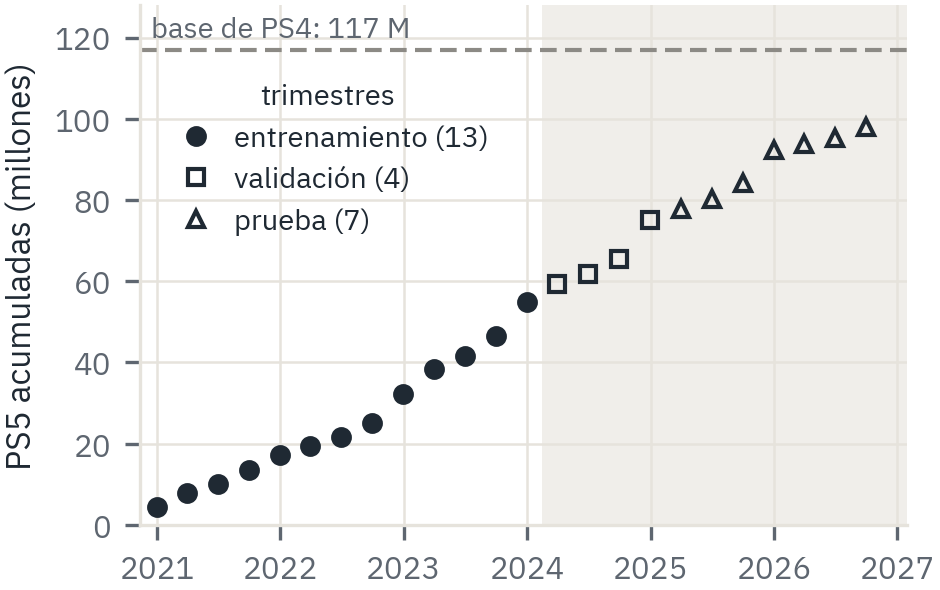
\includegraphics[width=\linewidth]{serie_ps5.png}
    \end{column}
    \begin{column}{0.36\textwidth}
      {\small\begin{itemize}
        \item \cifraPsUnidadesIni\ a \cifraPsUnidadesFin\ millones acumulados, dic.\,2020 a sep.\,2026.
        \item Adopción = acumulado / base de PS4 (\cifraUniverso\,M), fijada antes de ver la prueba.
        \item Simulación: \cifraCorridas\ corridas de 1000 agentes.
      \end{itemize}}
    \end{column}
  \end{columns}
  \fuente{Sony Interactive Entertainment, Business Data \& Sales (unidades vendidas a tiendas).}
\end{frame}
\note{\textbf{David (0:40).} La serie real son las unidades de PS5 que Sony publica cada trimestre: \cifraTrimestres\ trimestres, de \cifraPsUnidadesIni\ a \cifraPsUnidadesFin\ millones. La expresamos como porcentaje de la base de la PS4, \cifraUniverso\ millones, que fijamos antes de mirar los datos de prueba. El segundo conjunto lo genera la simulación: \cifraCorridas\ corridas de mil agentes.}

% =================================================================== 10. analogía GTA V
\begin{frame}{GTA\,6 aún no tiene ventas: lo parametrizamos con GTA\,V}
  \begin{columns}[c,totalwidth=\textwidth]
    \begin{column}{0.54\textwidth}
      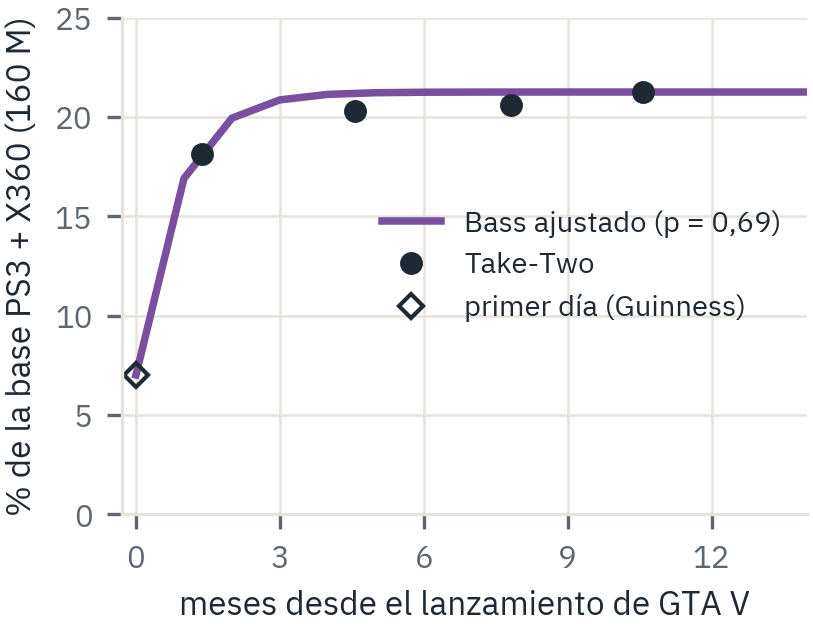
\includegraphics[width=0.94\linewidth]{analogia_gtav.png}
    \end{column}
    \begin{column}{0.42\textwidth}
      {\small\begin{itemize}
        \item GTA\,V: \cifraGtavSeisSemanas\,M en seis semanas y \cifraGtavMeseta\,M al año, sobre \cifraGtaBase\,M de consolas.
        \item Mismo ajuste de Bass: publicidad de \textcolor{terracota}{\cifraGtaP} al mes, unas \cifraGtaRazonPQ\ veces la imitación.
        \item GTA\,6 entre dueños de PS5: potencial \cifraGtaM\,\%, \cifraGtaIniciales\,\% el primer día, \cifraGtaHorizonte\ meses.
      \end{itemize}}
    \end{column}
  \end{columns}
  \fuente{Take-Two Interactive, resultados trimestrales 2013--2014; primer día: Guinness World Records (2013).}
\end{frame}
\note{\textbf{David (0:50).} GTA\,6 no tiene ventas todavía, así que usamos el método de analogía: tomamos el lanzamiento más parecido, GTA\,V. Vendió \cifraGtavSeisSemanas\ millones en seis semanas y se estabilizó en \cifraGtavMeseta\ millones, sobre \cifraGtaBase\ millones de consolas. Con la imitación fijada en la de la PS5, el ajuste atribuye el salto del lanzamiento a la publicidad: \cifraGtaP\ al mes, unas \cifraGtaRazonPQ\ veces la imitación, lo contrario de la PS5. Así modelamos GTA\,6 entre los dueños de PS5, con un potencial del \cifraGtaM\,\% y dos años de horizonte.}

% =================================================================== 11. diseño experimental
\renewcommand{\seccion}{Diseño experimental}
\begin{frame}{Cuatro experimentos, 30 réplicas por escenario}
  \vskip2mm
  \begin{tikzpicture}[x=1mm, y=1mm, font=\scriptsize]
    \fill[azul] (0,0) rectangle (60,10);
    \fill[azulclaro] (61,0) rectangle (92,10);
    \fill[terracota] (93,0) rectangle (134,10);
    \node[text=white, align=center] at (30,5) {entrenamiento\\dic.\,2020--dic.\,2023 · \cifraObsEnt\ trimestres};
    \node[text=tinta, align=center] at (76.5,5) {validación\\2024 · \cifraObsVal\ trimestres};
    \node[text=white, align=center] at (113.5,5) {prueba\\2025--2026 · \cifraObsPru\ trimestres};
    \node[text=secundario] at (30,-3) {ajusta $p$ y $q$};
    \node[text=secundario] at (76.5,-3) {elige $m$ y la red};
    \node[text=secundario] at (113.5,-3) {solo evalúa};
  \end{tikzpicture}
  \vskip6mm
  {\footnotesize
  \begin{tabular}{@{}lp{0.74\textwidth}r@{}}
    \toprule
    & factores (E1 a E3 para ambos casos: PS5 y GTA\,6) & corridas\\
    \midrule
    E1 & publicidad \{sin, con\} $\times$ densidad $k$ = 2, 4, 6, 8, 12, 16 & 720\\
    E2 & publicidad $\times$ topología \{aleatoria, mundo pequeño, libre de escala\} & 360\\
    E3 & duración de la campaña \{0, 1, 3, 6, 12, 24 meses, permanente\} & 420\\
    E4 & calibración PS5: 3 topologías $\times$ $k$ = 4, 8, 16 & 270\\
    \bottomrule
  \end{tabular}}
\end{frame}
\note{\textbf{David (0:50).} La serie de la PS5 se parte en el tiempo: con entrenamiento estimamos $p$ y $q$; como el potencial no se puede estimar en plena fase de crecimiento, lo elegimos en validación, igual que la red; la prueba solo evalúa. Corremos cuatro experimentos, los tres de escenarios para los dos casos: publicidad por densidad, publicidad por topología y duración de la campaña, más la calibración. Cada combinación se repite 30 veces. \emph{Duvan presenta las medidas y los resultados.}}

% =================================================================== 12. medidas
\renewcommand{\seccion}{Medidas de desempeño}
\begin{frame}{Cómo medimos}
  \vskip4mm
  \begin{columns}[T,totalwidth=\textwidth]
    \begin{column}{0.47\textwidth}
      {\plexmedia\color{azul}Escenarios}\par\vskip1mm
      {\small\begin{itemize}
        \item \alert{Adopción final}: \% de la población que adoptó al final del período (PS5: \cifraHorizontePs\ meses; GTA\,6: \cifraHorizonteGta).
        \item Mes del 50\,\% y mes del pico de compras.
        \item Media e IC del 95\,\% con 30 réplicas.
      \end{itemize}}
    \end{column}
    \begin{column}{0.47\textwidth}
      {\plexmedia\color{azul}Ajuste a la serie real}\par\vskip1mm
      {\small\begin{itemize}
        \item RMSE: raíz del error cuadrático medio, en puntos porcentuales.
        \item MAPE: error porcentual absoluto medio.
        \item Por partición: entrenamiento, validación y prueba.
      \end{itemize}}
    \end{column}
  \end{columns}
\end{frame}
\note{\textbf{Duvan (0:30).} La medida principal, la que pide el enunciado, es el porcentaje de adopción al final del período: seis años para la PS5 y dos para GTA\,6. La complementamos con el mes del 50\,\% y el mes del pico de compras. Frente a la serie real usamos RMSE y MAPE por partición. Todo con 30 réplicas e intervalos del 95\,\%.}

% =================================================================== 13. calibración
\renewcommand{\seccion}{Resultados}
\begin{frame}{El modelo sigue la serie de prueba de la PS5}
  \begin{columns}[c,totalwidth=\textwidth]
    \begin{column}{0.64\textwidth}
      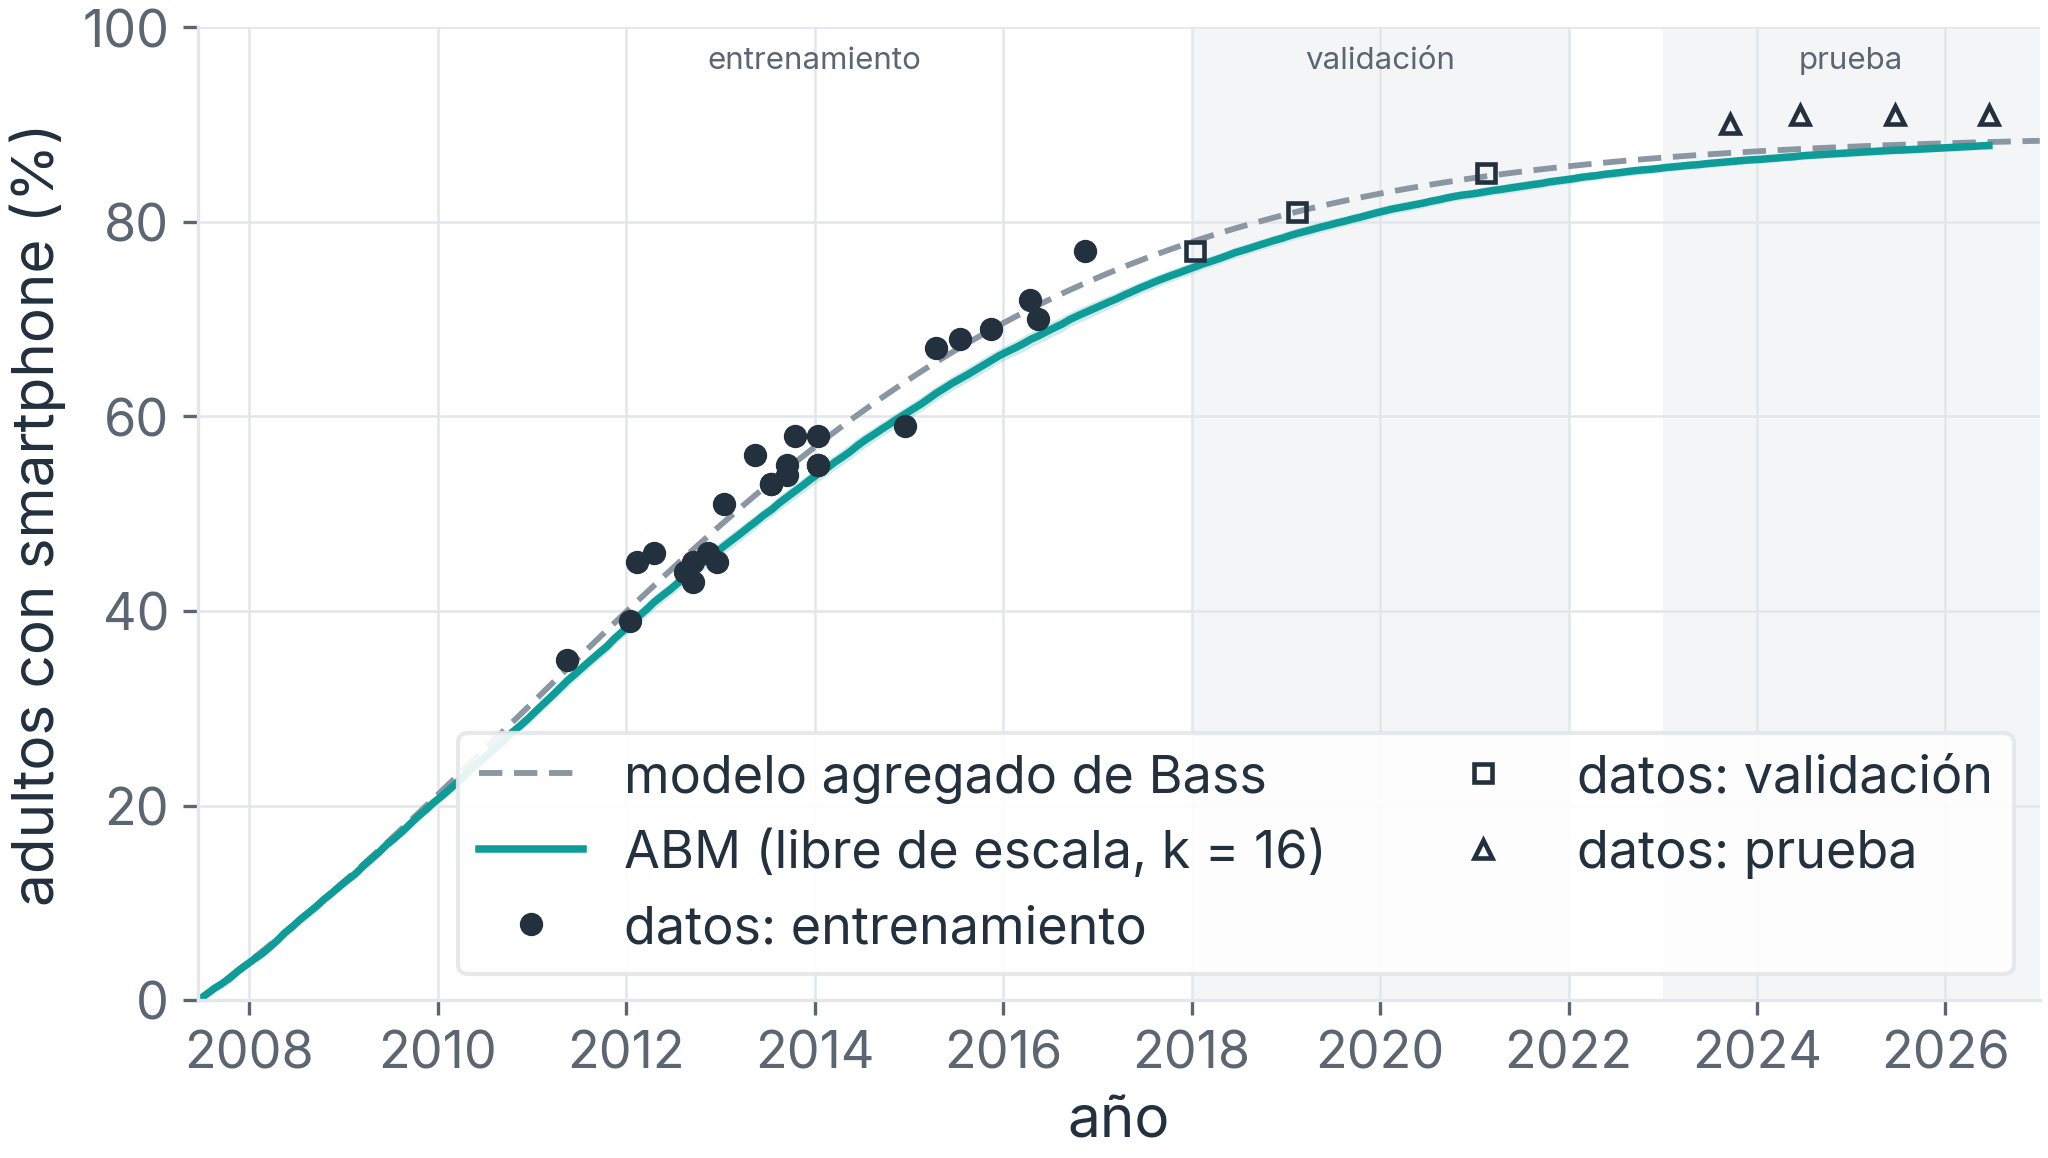
\includegraphics[width=\linewidth]{fig_calibracion.png}
    \end{column}
    \begin{column}{0.32\textwidth}
      \cifra{\cifraAbmRmsePru\ pp}{error en prueba del modelo de agentes (Bass: \cifraBassRmsePru)}\par\vskip5mm
      \nota{Bass anual: $p$\,=\,\cifraBassP, $q$\,=\,\cifraBassQ; la imitación pesa \cifraBassRazonQP\ veces más. Red elegida en validación: \cifraAbmSelRedNombre, $k$\,=\,\cifraAbmSelK.}
    \end{column}
  \end{columns}
\end{frame}
\note{\textbf{Duvan (0:50).} El ajuste da $p$ = \cifraBassP\ y $q$ = \cifraBassQ\ anuales: en la PS5 la imitación pesa \cifraBassRazonQP\ veces más que la publicidad. En validación se eligió la \cifraAbmSelRedNombre\ con $k$ = \cifraAbmSelK. En prueba, que nunca usamos para ajustar, el error es de \cifraAbmRmsePru\ puntos, mayor que el de Bass, \cifraBassRmsePru, porque la red frena la difusión. Ambos quedan un poco por debajo del dato de Sony de noviembre de 2026, más de 100 millones: la PS5 probablemente superará la base de la PS4.}

% =================================================================== 14. publicidad
\begin{frame}{Sin publicidad, ninguno de los dos llega lejos}
  \vskip1mm
  \begin{center}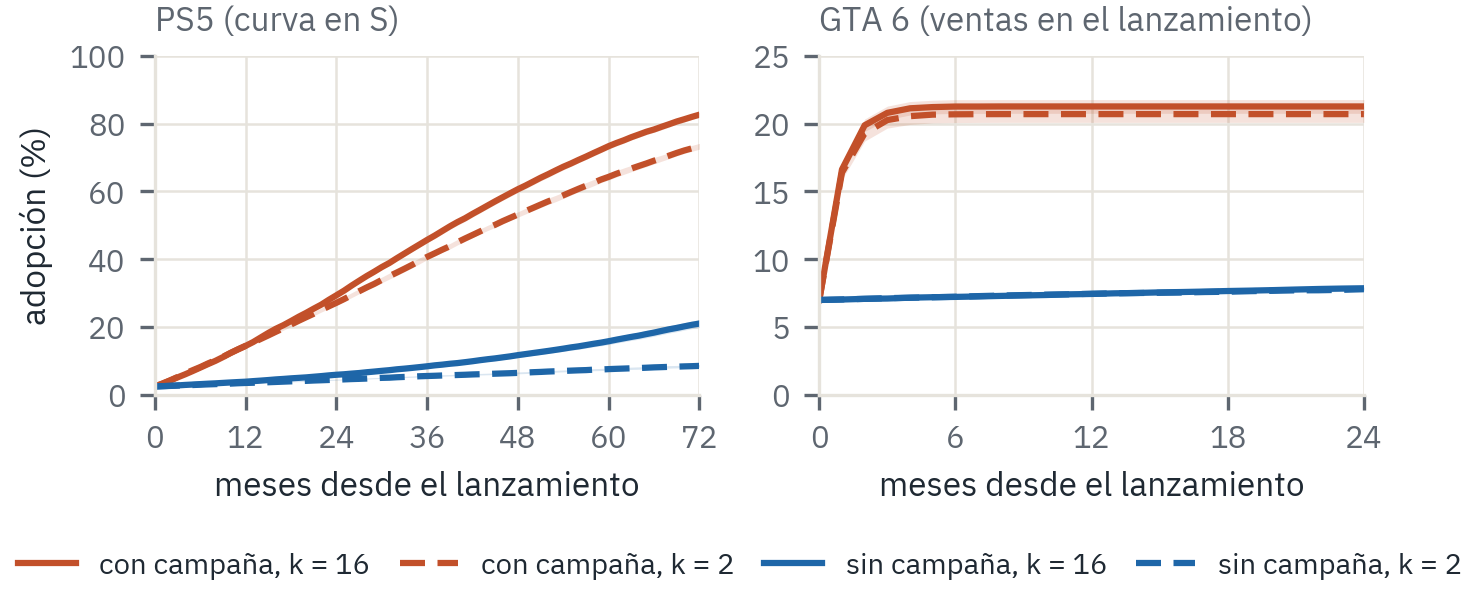
\includegraphics[width=0.9\linewidth]{publicidad_casos.png}\end{center}
  \vskip-3mm
  \nota{Red de mundo pequeño con $k$\,=\,2 (discontinua) y 16 (continua).}
\end{frame}
\note{\textbf{Duvan (0:50).} El resultado central. En la PS5, sin publicidad la adopción queda entre el \cifraPsSinMin\ y el \cifraPsSinMax\,\% en seis años; con campaña, entre el \cifraPsConMin\ y el \cifraPsConMax\,\%, con la curva en S. En GTA\,6 la campaña lo decide todo: con ella se alcanza el potencial casi en el primer mes; sin ella la adopción apenas pasa de los compradores del primer día. Sin publicidad, la PS5 simplemente no despega.}

% =================================================================== 15. densidad y topología
\begin{frame}{La red pesa sobre todo cuando no hay publicidad}
  \begin{columns}[c,totalwidth=\textwidth]
    \begin{column}{0.66\textwidth}
      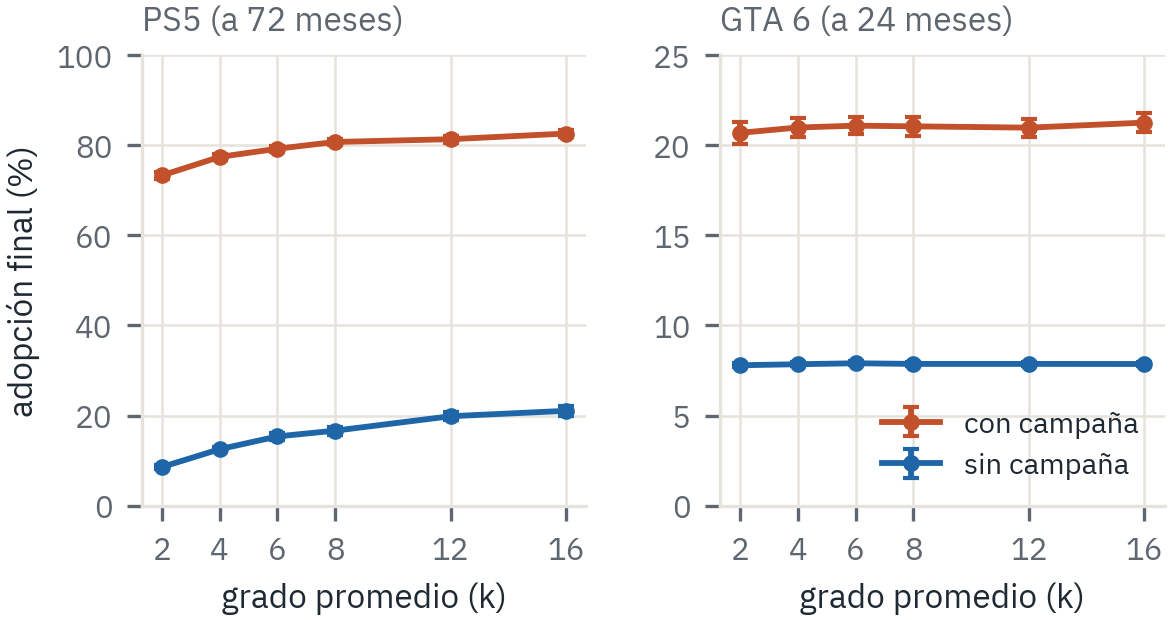
\includegraphics[width=\linewidth]{densidad.png}
    \end{column}
    \begin{column}{0.3\textwidth}
      \cifra{×\,\cifraPsSinRazon}{adopción de la PS5 sin campaña al pasar de $k$\,=\,2 a 16}\par\vskip4mm
      \nota{Con campaña, la misma diferencia solo la multiplica por \cifraPsConRazon. Sin campaña, la red de mundo pequeño es la topología más lenta.}
    \end{column}
  \end{columns}
\end{frame}
\note{\textbf{Duvan (0:50).} En la PS5 sin publicidad, pasar de 2 a 16 contactos multiplica la adopción por \cifraPsSinRazon; con campaña solo por \cifraPsConRazon, porque la publicidad siembra adoptantes en toda la red. En la topología pasa lo mismo: sin campaña, la red de mundo pequeño es la más lenta de las tres, porque sus grupos cerrados atrapan la influencia, y la libre de escala la más variable, porque depende de si un nodo muy conectado adopta temprano. En GTA\,6 la red casi no cambia nada.}

% =================================================================== 16. duración
\begin{frame}{GTA\,6: basta un mes; PS5: la campaña necesita tiempo}
  \begin{columns}[c,totalwidth=\textwidth]
    \begin{column}{0.58\textwidth}
      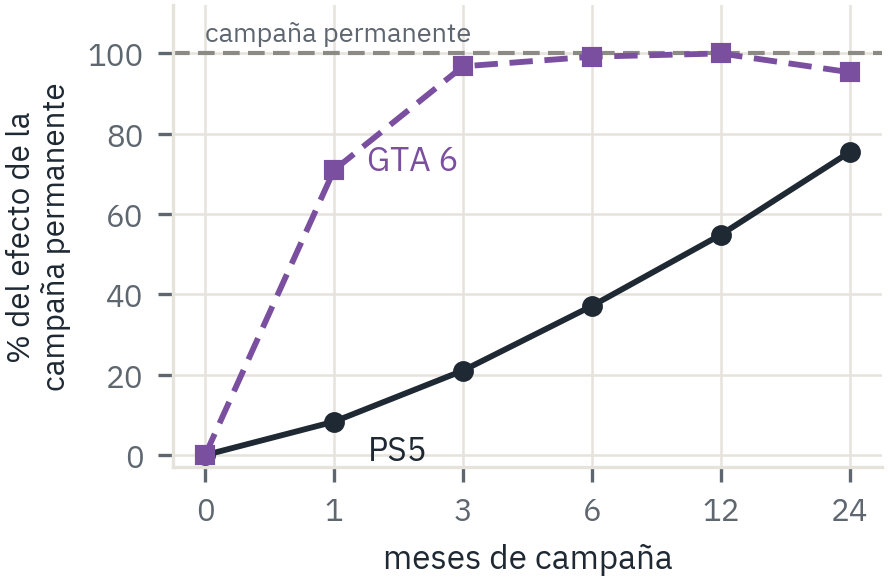
\includegraphics[width=\linewidth]{fraccion_duracion.png}
    \end{column}
    \begin{column}{0.38\textwidth}
      \cifra{\cifraFraccionGtaDUno\,\%}{del efecto de una campaña permanente se logra con un mes en GTA\,6}\par\vskip5mm
      \cifra{\cifraFraccionPsDDoce\,\%}{se logra con un año en la PS5 (dos años: \cifraFraccionPsDVeinticuatro\,\%)}
    \end{column}
  \end{columns}
\end{frame}
\note{\textbf{Duvan (0:40).} Si la campaña se corta, ¿cuánto se pierde? En GTA\,6, un solo mes ya logra el \cifraFraccionGtaDUno\,\% del efecto de una campaña permanente: el lanzamiento concentra casi todo. En la PS5 el rendimiento es gradual: un año logra el \cifraFraccionPsDDoce\,\% y dos años el \cifraFraccionPsDVeinticuatro\,\%, porque la imitación necesita tiempo para sostener la difusión. Los puntos de GTA\,6 que pasan apenas del 100\,\% son variación entre réplicas. \emph{David hace la demostración.}}

% =================================================================== 17. demo
\renewcommand{\seccion}{Demostración}
\begin{frame}{En vivo en NetLogo}
  \vskip1mm
  \begin{columns}[c,totalwidth=\textwidth]
    \begin{column}{0.4\textwidth}
      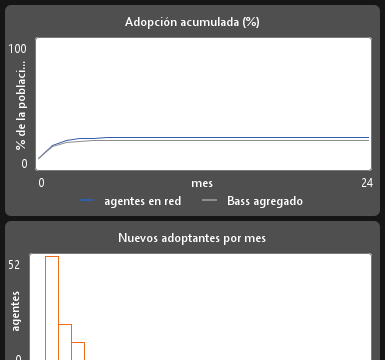
\includegraphics[width=0.86\linewidth]{netlogo_gta6.png}\par\vskip1mm
      {\fontsize{6}{7}\selectfont\color{tenue}Caso GTA\,6: compras concentradas en el primer mes.}
    \end{column}
    \begin{column}{0.56\textwidth}
      {\small\begin{enumerate}
        \item Caso \alert{GTA\,6} $\to$ configurar $\to$ simular: el pico llega en el primer mes.
        \item Campaña apagada: la adopción apenas pasa del \cifraGtaIniciales\,\%.
        \item Caso \textcolor{azul}{PS5}: curva en S frente a la de Bass.
      \end{enumerate}}
      \vskip2mm
      \nota{Si sobra tiempo: PS5 sin campaña y $k$ de 16 a 2; Herramientas $\to$ BehaviorSpace.}
    \end{column}
  \end{columns}
\end{frame}
\note{\textbf{David (1:10).} Demostración en vivo; los pasos están en el guion. Hacer 1 a 3; los otros dos solo si sobra tiempo.}

% =================================================================== 18. conclusiones
\renewcommand{\seccion}{Conclusiones}
\begin{frame}{Publicidad primero, red después}
  \vskip2mm
  \begin{enumerate}
    \item PS5: sin campaña, a lo sumo \cifraPsSinMaxGlobal\,\%; con campaña, al menos \cifraPsConMin\,\%.
    \item GTA\,6: un mes de campaña logra el \cifraFraccionGtaDUno\,\% del efecto.
    \item La red pesa sobre todo cuando no hay publicidad.
    \item Error en prueba: \cifraAbmRmsePru\ pp; la reimplementación en Python coincide.
  \end{enumerate}
  \vskip5mm
  \nota{Limitaciones: coeficientes iguales para todos, red fija, unidades vendidas a tiendas y parámetros de GTA\,6 hipotéticos.}
\end{frame}
\note{\textbf{Duvan (0:30).} Cuatro conclusiones. En la PS5, la publicidad es la condición del despegue. En GTA\,6, el primer mes de campaña decide el resultado. La red pesa sobre todo cuando no hay publicidad. Y el modelo quedó validado con datos que no usamos para ajustar y verificado con una reimplementación independiente.}

% =================================================================== 19. referencias
\renewcommand{\seccion}{Referencias}
\begin{frame}{Fuentes}
  \vskip0.5mm
  \raggedright\fontsize{8}{9.6}\selectfont
  \setlength{\parskip}{1.1mm}
  \referencia{Bass, F.\,M. (1969). A new product growth model for consumer durables. \textit{Management Science}, 15(5), 215--227.}
  \referencia{Goldenberg, J., Libai, B. y Muller, E. (2001). Talk of the network. \textit{Marketing Letters}, 12(3), 211--223.}
  \referencia{Rogers, E.\,M. (2003). \textit{Diffusion of Innovations} (5.ª ed.). Free Press.}
  \referencia{Thomas, R.\,J. (1985). Estimating market growth for new products: an analogical diffusion model approach. \textit{Journal of Product Innovation Management}, 2(1), 45--55.}
  \referencia{Watts, D.\,J. y Strogatz, S.\,H. (1998). Collective dynamics of `small-world' networks. \textit{Nature}, 393, 440--442.}
  \referencia{Wilensky, U. (1999). NetLogo. Northwestern University.}
  \referencia{Sony Interactive Entertainment (2026). Business Data \& Sales.}
  \referencia{Take-Two Interactive (2013--2014). Resultados trimestrales, años fiscales 2014 y 2015.}
  \referencia{Guinness World Records (2013, 2023). Récords de ventas de GTA\,V y de vistas del tráiler de GTA\,6.}
\end{frame}
\note{\textbf{Duvan (0:10).} Las referencias están en pantalla. Gracias; quedamos atentos a sus preguntas.}

\end{document}
"  -> notas del orador
% Las cifras salen de ../articulo/tablas/cifras.tex (analisis/analisis_resultados.py) y las
% figuras de ../analisis/figuras/diapositivas (analisis/figuras_diapositivas.py).
\ifdefined\connotas
  \documentclass[aspectratio=169,11pt,notes=only]{beamer}
\else
  \documentclass[aspectratio=169,11pt]{beamer}
\fi

\usepackage{fontspec}
\usepackage[spanish,es-noshorthands]{babel}
\usepackage{booktabs}
\usepackage{tikz}
\usepackage{listings}
\usetikzlibrary{arrows.meta,positioning,calc,fit,backgrounds}

% ------------------------------------------------------------------ tipografía
\setsansfont{IBMPlexSans}[Path=../analisis/fuentes/, Extension=.ttf, UprightFont=*-Regular,
  BoldFont=*-SemiBold, ItalicFont=*-Regular, ItalicFeatures={FakeSlant=0.18}]
\newfontfamily\plexmedia{IBMPlexSans-Medium}[Path=../analisis/fuentes/, Extension=.ttf]
\usefonttheme{professionalfonts}
\usefonttheme[onlymath]{serif}
\hyphenpenalty=10000
\exhyphenpenalty=10000

% ------------------------------------------------------------------ colores
% terracota = publicidad (con campaña), azul = imitación (sin campaña), igual que en el modelo y las figuras
\definecolor{papel}{HTML}{FBFAF6}
\definecolor{tinta}{HTML}{1F2933}
\definecolor{secundario}{HTML}{5E6670}
\definecolor{tenue}{HTML}{8C8A85}
\definecolor{borde}{HTML}{B9B4AA}
\definecolor{claro}{HTML}{F1EEE7}
\definecolor{azul}{HTML}{1E66A8}
\definecolor{azulclaro}{HTML}{8DB3D6}
\definecolor{azulfondo}{HTML}{E4EDF6}
\definecolor{terracota}{HTML}{C2502A}
\definecolor{terracotafondo}{HTML}{F7E6DE}

\setbeamercolor{background canvas}{bg=papel}
\setbeamercolor{normal text}{fg=tinta}
\setbeamercolor{structure}{fg=azul}
\setbeamercolor{frametitle}{fg=tinta}
\setbeamercolor{alerted text}{fg=terracota}
\setbeamercolor{item}{fg=terracota}
\setbeamercolor{enumerate item}{fg=terracota}

% ------------------------------------------------------------------ plantillas
\setbeamertemplate{navigation symbols}{}
\setbeamersize{text margin left=13mm, text margin right=13mm}
\setbeamerfont{frametitle}{size=\Large}
\newcommand{\seccion}{}
\setbeamertemplate{frametitle}{%
  \vskip6mm%
  {\scriptsize\addfontfeatures{LetterSpace=12}\color{terracota}\MakeUppercase{\seccion}}\par\vskip1mm%
  {\usebeamerfont{frametitle}\plexmedia\color{tinta}\insertframetitle\par}\vskip0.5mm}
\setbeamertemplate{footline}{%
  \hbox to \paperwidth{\hskip13mm{\fontsize{6}{7}\selectfont\color{tenue}Delgado · Monroy · Baquero\quad Universidad de los Llanos}%
  \hfill{\fontsize{6}{7}\selectfont\color{tenue}\insertframenumber\,/\,\inserttotalframenumber}\hskip13mm}\vskip4mm}
\setbeamertemplate{itemize item}{\raisebox{0.3ex}{\color{terracota}\rule{0.8ex}{0.8ex}}}
\setbeamertemplate{enumerate item}{\color{terracota}\plexmedia\insertenumlabel.}
\setbeamertemplate{itemize/enumerate body begin}{\raggedright}
\setlength{\leftmargini}{1.3em}
\setbeamertemplate{note page}{\vskip5mm\hskip6mm\begin{minipage}[t]{0.42\paperwidth}\vskip0pt\insertslideintonotes{0.4}\end{minipage}%
  \hskip4mm\begin{minipage}[t]{0.4\paperwidth}\vskip0pt\raggedright\footnotesize
  {\scriptsize\color{terracota}DIAPOSITIVA \insertframenumber}\par\vskip2mm\insertnote\end{minipage}}

\lstset{basicstyle=\ttfamily\fontsize{7.2}{8.6}\selectfont\color{tinta}, keywordstyle=\color{azul}, columns=fullflexible,
  keepspaces=true, frame=none, aboveskip=0pt, belowskip=0pt,
  morekeywords={to,end,ask,let,set,if,with,count,any?,random-float,turtles,link-neighbors,not}}

% ------------------------------------------------------------------ utilidades
\newcommand{\cifra}[2]{% número grande + leyenda
  \begin{minipage}[t]{\linewidth}\raggedright{\plexmedia\fontsize{24}{26}\selectfont\color{azul}#1\par}\vskip1mm
  {\small\color{secundario}#2\par}\end{minipage}}
\newcommand{\nota}[1]{{\raggedright\footnotesize\color{secundario}#1\par}}
\newcommand{\fuente}[1]{\par\vfill{\fontsize{6}{7}\selectfont\color{tenue}#1}\par\vskip1mm}
\newcommand{\referencia}[1]{\par\hangindent=1.4em\hangafter=1 #1\par}

% generado por analisis_resultados.py
\newcommand{\cifraBassP}{0,079}
\newcommand{\cifraBassQ}{0,242}
\newcommand{\cifraBassM}{89}
\newcommand{\cifraBassPmes}{0,0066}
\newcommand{\cifraBassQmes}{0,0202}
\newcommand{\cifraBassPico}{3,5}
\newcommand{\cifraBassRmseEnt}{2,29}
\newcommand{\cifraBassMapeEnt}{3,64}
\newcommand{\cifraBassRmseVal}{0,63}
\newcommand{\cifraBassMapeVal}{0,60}
\newcommand{\cifraBassRmsePru}{3,10}
\newcommand{\cifraBassMapePru}{3,40}
\newcommand{\cifraAbmSelRed}{libre de escala}
\newcommand{\cifraAbmSelK}{16}
\newcommand{\cifraAbmRmseEnt}{3,52}
\newcommand{\cifraAbmRmseVal}{1,93}
\newcommand{\cifraAbmRmsePru}{3,74}
\newcommand{\cifraAbmMapePru}{4,10}
\newcommand{\cifraAbmFinal}{87,8}
\newcommand{\cifraAbmRmseValMax}{4,90}
\newcommand{\cifraAbmRmsePruMax}{5,37}
\newcommand{\cifraAbmPeorRed}{aleatoria}
\newcommand{\cifraAbmPeorK}{4}
\newcommand{\cifraSinCalKDos}{8,1}
\newcommand{\cifraSinCalKDosIc}{0,3}
\newcommand{\cifraTcincuentaSinCalKDos}{--}
\newcommand{\cifraSinCalKCuatro}{11,2}
\newcommand{\cifraSinCalKCuatroIc}{0,5}
\newcommand{\cifraTcincuentaSinCalKCuatro}{--}
\newcommand{\cifraSinCalKSeis}{13,2}
\newcommand{\cifraSinCalKSeisIc}{0,7}
\newcommand{\cifraTcincuentaSinCalKSeis}{--}
\newcommand{\cifraSinCalKOcho}{14,9}
\newcommand{\cifraSinCalKOchoIc}{0,8}
\newcommand{\cifraTcincuentaSinCalKOcho}{--}
\newcommand{\cifraSinCalKDoce}{15,1}
\newcommand{\cifraSinCalKDoceIc}{0,8}
\newcommand{\cifraTcincuentaSinCalKDoce}{--}
\newcommand{\cifraSinCalKDieciseis}{16,9}
\newcommand{\cifraSinCalKDieciseisIc}{1,0}
\newcommand{\cifraTcincuentaSinCalKDieciseis}{--}
\newcommand{\cifraConCalKDos}{79,8}
\newcommand{\cifraConCalKDosIc}{0,6}
\newcommand{\cifraTcincuentaConCalKDos}{63}
\newcommand{\cifraConCalKCuatro}{82,9}
\newcommand{\cifraConCalKCuatroIc}{0,5}
\newcommand{\cifraTcincuentaConCalKCuatro}{62}
\newcommand{\cifraConCalKSeis}{83,8}
\newcommand{\cifraConCalKSeisIc}{0,6}
\newcommand{\cifraTcincuentaConCalKSeis}{59}
\newcommand{\cifraConCalKOcho}{84,4}
\newcommand{\cifraConCalKOchoIc}{0,6}
\newcommand{\cifraTcincuentaConCalKOcho}{59}
\newcommand{\cifraConCalKDoce}{85,5}
\newcommand{\cifraConCalKDoceIc}{0,5}
\newcommand{\cifraTcincuentaConCalKDoce}{58}
\newcommand{\cifraConCalKDieciseis}{85,4}
\newcommand{\cifraConCalKDieciseisIc}{0,6}
\newcommand{\cifraTcincuentaConCalKDieciseis}{59}
\newcommand{\cifraSinLitKDos}{11,8}
\newcommand{\cifraSinLitKDosIc}{0,5}
\newcommand{\cifraTcincuentaSinLitKDos}{--}
\newcommand{\cifraSinLitKCuatro}{18,9}
\newcommand{\cifraSinLitKCuatroIc}{0,7}
\newcommand{\cifraTcincuentaSinLitKCuatro}{--}
\newcommand{\cifraSinLitKSeis}{24,2}
\newcommand{\cifraSinLitKSeisIc}{0,8}
\newcommand{\cifraTcincuentaSinLitKSeis}{--}
\newcommand{\cifraSinLitKOcho}{27,0}
\newcommand{\cifraSinLitKOchoIc}{1,1}
\newcommand{\cifraTcincuentaSinLitKOcho}{--}
\newcommand{\cifraSinLitKDoce}{35,0}
\newcommand{\cifraSinLitKDoceIc}{1,2}
\newcommand{\cifraTcincuentaSinLitKDoce}{--}
\newcommand{\cifraSinLitKDieciseis}{35,9}
\newcommand{\cifraSinLitKDieciseisIc}{1,5}
\newcommand{\cifraTcincuentaSinLitKDieciseis}{--}
\newcommand{\cifraConLitKDos}{87,7}
\newcommand{\cifraConLitKDosIc}{0,6}
\newcommand{\cifraTcincuentaConLitKDos}{54}
\newcommand{\cifraConLitKCuatro}{91,3}
\newcommand{\cifraConLitKCuatroIc}{0,4}
\newcommand{\cifraTcincuentaConLitKCuatro}{52}
\newcommand{\cifraConLitKSeis}{93,2}
\newcommand{\cifraConLitKSeisIc}{0,4}
\newcommand{\cifraTcincuentaConLitKSeis}{48}
\newcommand{\cifraConLitKOcho}{93,8}
\newcommand{\cifraConLitKOchoIc}{0,3}
\newcommand{\cifraTcincuentaConLitKOcho}{48}
\newcommand{\cifraConLitKDoce}{94,0}
\newcommand{\cifraConLitKDoceIc}{0,3}
\newcommand{\cifraTcincuentaConLitKDoce}{48}
\newcommand{\cifraConLitKDieciseis}{94,2}
\newcommand{\cifraConLitKDieciseisIc}{0,4}
\newcommand{\cifraTcincuentaConLitKDieciseis}{48}
\newcommand{\cifraDensidadGananciaCon}{6}
\newcommand{\cifraDensidadRazonSinCal}{2,1}
\newcommand{\cifraDensidadRazonSinLit}{3,0}
\newcommand{\cifraTopoSinCalAleatoria}{15,4}
\newcommand{\cifraTopoSinCalAleatoriaIc}{0,9}
\newcommand{\cifraTopoSinCalAleatoriaDe}{2,3}
\newcommand{\cifraTopoSinCalAleatoriaProp}{0}
\newcommand{\cifraTopoSinCalEscala}{13,1}
\newcommand{\cifraTopoSinCalEscalaIc}{1,2}
\newcommand{\cifraTopoSinCalEscalaDe}{3,3}
\newcommand{\cifraTopoSinCalEscalaProp}{0}
\newcommand{\cifraTopoSinCalMundo}{12,9}
\newcommand{\cifraTopoSinCalMundoIc}{0,5}
\newcommand{\cifraTopoSinCalMundoDe}{1,4}
\newcommand{\cifraTopoSinCalMundoProp}{0}
\newcommand{\cifraTopoConCalAleatoria}{83,6}
\newcommand{\cifraTopoConCalAleatoriaIc}{0,6}
\newcommand{\cifraTopoConCalAleatoriaDe}{1,5}
\newcommand{\cifraTopoConCalAleatoriaProp}{100}
\newcommand{\cifraTopoConCalEscala}{84,5}
\newcommand{\cifraTopoConCalEscalaIc}{0,7}
\newcommand{\cifraTopoConCalEscalaDe}{1,9}
\newcommand{\cifraTopoConCalEscalaProp}{100}
\newcommand{\cifraTopoConCalMundo}{83,8}
\newcommand{\cifraTopoConCalMundoIc}{0,7}
\newcommand{\cifraTopoConCalMundoDe}{2,0}
\newcommand{\cifraTopoConCalMundoProp}{100}
\newcommand{\cifraTopoSinLitAleatoria}{33,3}
\newcommand{\cifraTopoSinLitAleatoriaIc}{2,1}
\newcommand{\cifraTopoSinLitAleatoriaDe}{5,6}
\newcommand{\cifraTopoSinLitAleatoriaProp}{0}
\newcommand{\cifraTopoSinLitEscala}{34,2}
\newcommand{\cifraTopoSinLitEscalaIc}{2,9}
\newcommand{\cifraTopoSinLitEscalaDe}{7,8}
\newcommand{\cifraTopoSinLitEscalaProp}{3}
\newcommand{\cifraTopoSinLitMundo}{23,4}
\newcommand{\cifraTopoSinLitMundoIc}{1,1}
\newcommand{\cifraTopoSinLitMundoDe}{2,8}
\newcommand{\cifraTopoSinLitMundoProp}{0}
\newcommand{\cifraTopoConLitAleatoria}{93,3}
\newcommand{\cifraTopoConLitAleatoriaIc}{0,4}
\newcommand{\cifraTopoConLitAleatoriaDe}{1,1}
\newcommand{\cifraTopoConLitAleatoriaProp}{100}
\newcommand{\cifraTopoConLitEscala}{93,3}
\newcommand{\cifraTopoConLitEscalaIc}{0,3}
\newcommand{\cifraTopoConLitEscalaDe}{0,9}
\newcommand{\cifraTopoConLitEscalaProp}{100}
\newcommand{\cifraTopoConLitMundo}{92,7}
\newcommand{\cifraTopoConLitMundoIc}{0,4}
\newcommand{\cifraTopoConLitMundoDe}{1,1}
\newcommand{\cifraTopoConLitMundoProp}{100}
\newcommand{\cifraDurCalDCero}{13,0}
\newcommand{\cifraDurCalDCeroIc}{0,7}
\newcommand{\cifraTcincuentaDurCalDCero}{--}
\newcommand{\cifraDurCalDSeis}{28,5}
\newcommand{\cifraDurCalDSeisIc}{0,9}
\newcommand{\cifraTcincuentaDurCalDSeis}{--}
\newcommand{\cifraDurCalDDoce}{41,0}
\newcommand{\cifraDurCalDDoceIc}{1,4}
\newcommand{\cifraTcincuentaDurCalDDoce}{--}
\newcommand{\cifraDurCalDVeinticuatro}{54,6}
\newcommand{\cifraDurCalDVeinticuatroIc}{1,2}
\newcommand{\cifraTcincuentaDurCalDVeinticuatro}{107}
\newcommand{\cifraDurCalDSesenta}{74,2}
\newcommand{\cifraDurCalDSesentaIc}{0,7}
\newcommand{\cifraTcincuentaDurCalDSesenta}{59}
\newcommand{\cifraDurCalDCientoveinte}{84,4}
\newcommand{\cifraDurCalDCientoveinteIc}{0,6}
\newcommand{\cifraTcincuentaDurCalDCientoveinte}{59}
\newcommand{\cifraDurLitDCero}{23,9}
\newcommand{\cifraDurLitDCeroIc}{1,1}
\newcommand{\cifraTcincuentaDurLitDCero}{--}
\newcommand{\cifraDurLitDSeis}{46,9}
\newcommand{\cifraDurLitDSeisIc}{1,9}
\newcommand{\cifraTcincuentaDurLitDSeis}{--}
\newcommand{\cifraDurLitDDoce}{60,9}
\newcommand{\cifraDurLitDDoceIc}{1,1}
\newcommand{\cifraTcincuentaDurLitDDoce}{98}
\newcommand{\cifraDurLitDVeinticuatro}{74,5}
\newcommand{\cifraDurLitDVeinticuatroIc}{1,1}
\newcommand{\cifraTcincuentaDurLitDVeinticuatro}{72}
\newcommand{\cifraDurLitDSesenta}{88,1}
\newcommand{\cifraDurLitDSesentaIc}{0,7}
\newcommand{\cifraTcincuentaDurLitDSesenta}{50}
\newcommand{\cifraDurLitDCientoveinte}{93,0}
\newcommand{\cifraDurLitDCientoveinteIc}{0,3}
\newcommand{\cifraTcincuentaDurLitDCientoveinte}{50}
\newcommand{\cifraEstAleatoriaC}{0,006}
\newcommand{\cifraEstAleatoriaL}{4,0}
\newcommand{\cifraEstEscalaC}{0,032}
\newcommand{\cifraEstEscalaL}{3,5}
\newcommand{\cifraEstMundoC}{0,444}
\newcommand{\cifraEstMundoL}{6,2}
\newcommand{\cifraSinCalMin}{8,1}
\newcommand{\cifraSinCalMax}{16,9}
\newcommand{\cifraSinLitMin}{11,8}
\newcommand{\cifraSinLitMax}{35,9}
\newcommand{\cifraConCalMin}{79,8}
\newcommand{\cifraConCalMax}{85,5}
\newcommand{\cifraConLitMin}{87,7}
\newcommand{\cifraConLitMax}{94,2}
\newcommand{\cifraTopoSinCalMin}{12,9}
\newcommand{\cifraTopoSinCalMax}{15,4}
\newcommand{\cifraTopoSinLitMin}{23,4}
\newcommand{\cifraTopoSinLitMax}{34,2}
\newcommand{\cifraTopoConCalMin}{83,6}
\newcommand{\cifraTopoConCalMax}{84,5}
\newcommand{\cifraTopoConLitMin}{92,7}
\newcommand{\cifraTopoConLitMax}{93,3}
\newcommand{\cifraDurCalFraccionVeinticuatro}{58}
\newcommand{\cifraDurLitFraccionVeinticuatro}{73}
\newcommand{\cifraDurCalGananciaSeis}{15}
\newcommand{\cifraVerifEscenarios}{57}
\newcommand{\cifraVerifDifMedia}{0,5}
\newcommand{\cifraVerifDifMax}{2,7}
\newcommand{\cifraVerifSignif}{6}
\newcommand{\cifraVerifHolm}{ninguna diferencia es significativa}

\graphicspath{{figuras/}{../analisis/figuras/diapositivas/}{../articulo/figuras/}}

\begin{document}

% =================================================================== 1. portada
{\setbeamertemplate{footline}{}
\begin{frame}[plain]
  \begin{columns}[c,totalwidth=\textwidth]
    \begin{column}{0.62\textwidth}
      \raggedright
      {\scriptsize\addfontfeatures{LetterSpace=12}\color{terracota}PROYECTO 14 · SIMULACIÓN COMPUTACIONAL}\par\vskip5mm
      {\plexmedia\fontsize{21}{26}\selectfont\color{tinta}Publicidad y redes sociales en la difusión de innovaciones\par}\vskip3mm
      {\color{secundario}Un modelo basado en agentes de la PS5 y del lanzamiento de GTA\,6\par}\vskip8mm
      {\small Jesus Gregorio Delgado\\ David Andres Monroy Aguiar\\ Duvan Felipe Baquero Cerquera\par}\vskip5mm
      {\scriptsize\color{tenue}Ingeniería de Sistemas · Universidad de los Llanos\\ 17 de noviembre de 2026\par}
    \end{column}
    \begin{column}{0.36\textwidth}
      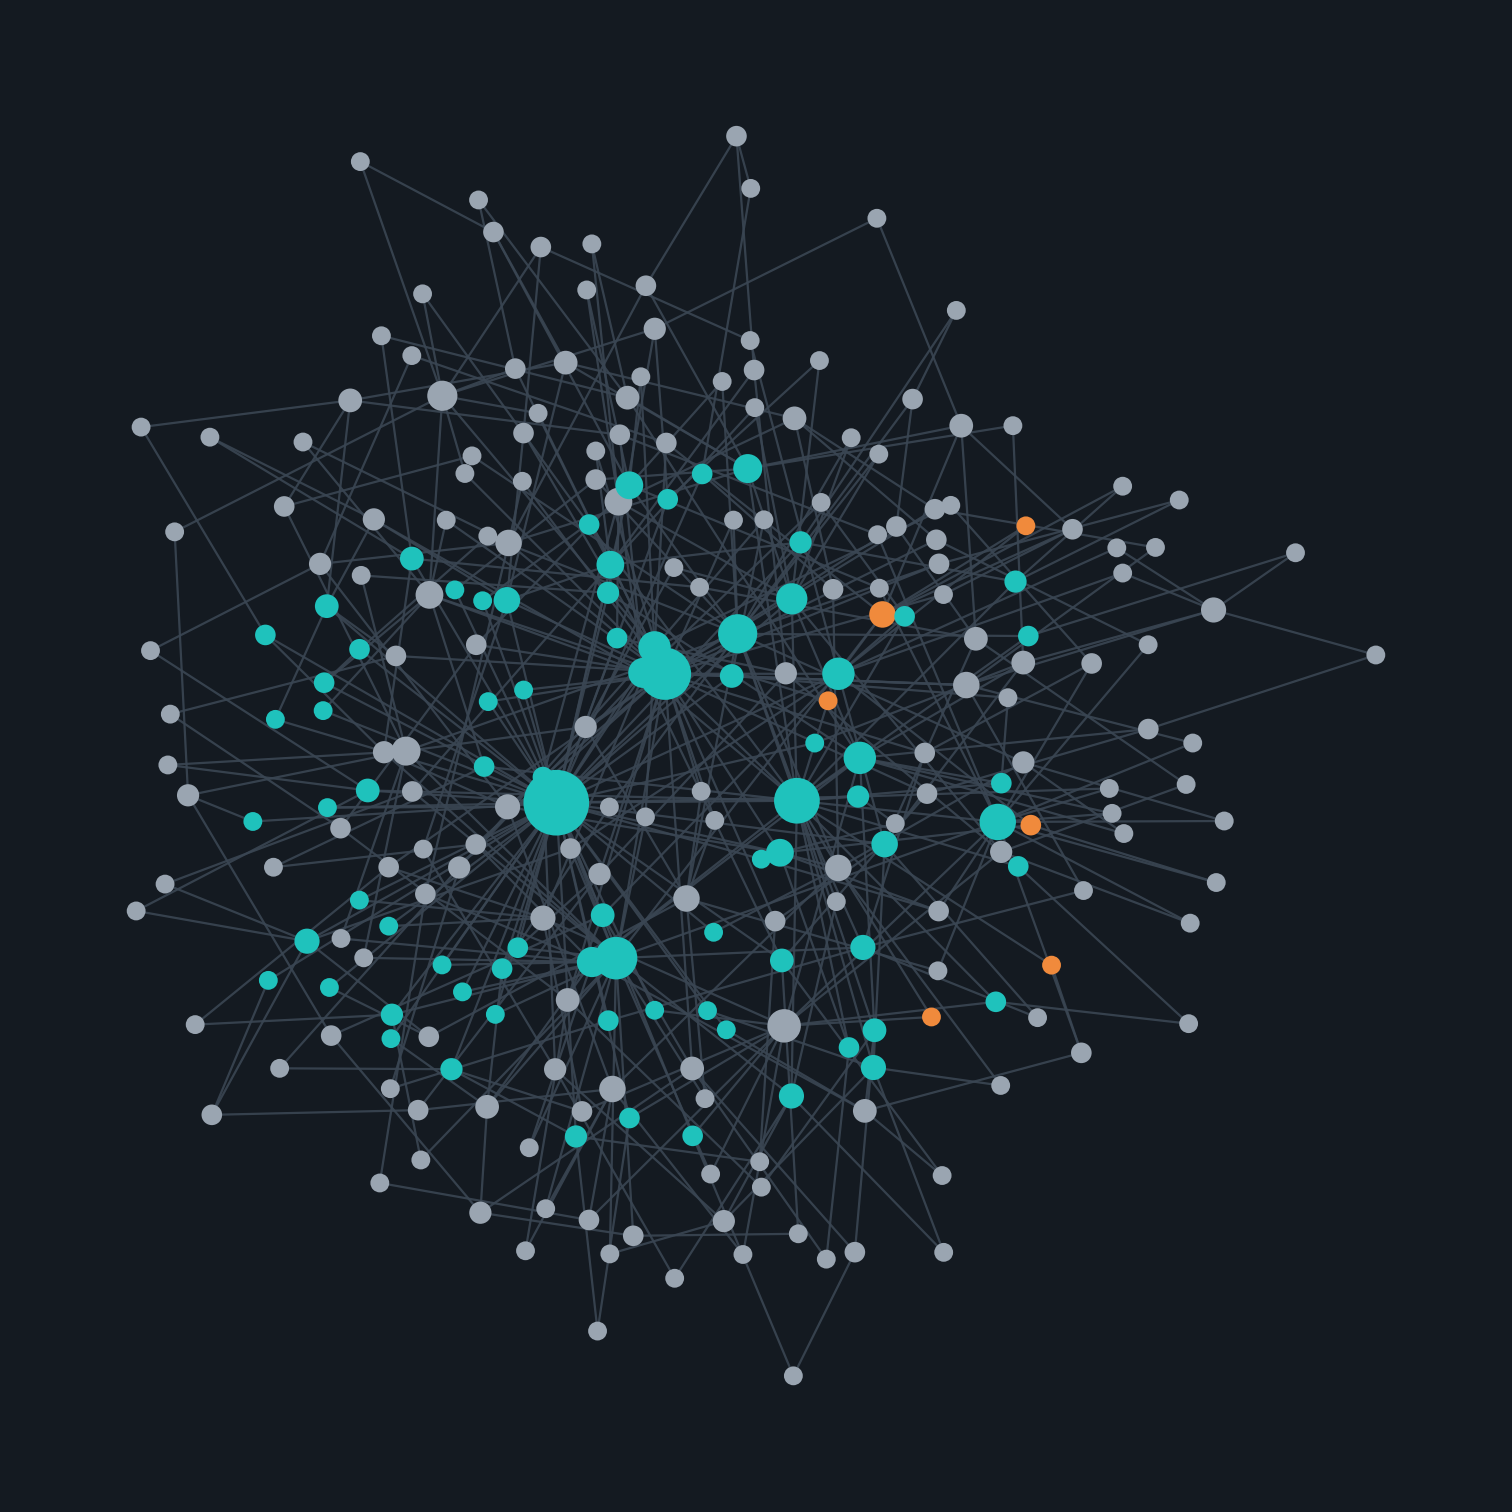
\includegraphics[width=\linewidth]{portada_red.png}
    \end{column}
  \end{columns}
\end{frame}
}
\note{\textbf{Jesus (0:40).} Buenos días. Somos Jesus, David y Duvan. Nuestro proyecto simula cómo se difunde un producto nuevo cuando cada persona decide influida por la publicidad y por sus contactos. Lo aplicamos a dos casos de actualidad: la PS5, una tecnología, y GTA\,6, un videojuego que sale este jueves. Lo construimos en NetLogo, lo calibramos con datos reales y lo usamos para comparar escenarios que no se pueden observar.}

% =================================================================== 2. motivación
\renewcommand{\seccion}{Motivación}
\begin{frame}{Dos lanzamientos, dos maneras de difundirse}
  \vskip4mm
  \begin{columns}[t,totalwidth=\textwidth]
    \begin{column}{0.31\textwidth}\cifra{\cifraPsUnidadesFin\,M}{PS5 vendidas de noviembre de 2020 a septiembre de 2026}\end{column}
    \begin{column}{0.31\textwidth}\cifra{19 nov.}{sale GTA\,6, solo para consolas de esta generación}\end{column}
    \begin{column}{0.31\textwidth}\cifra{90\,M}{vistas del primer tráiler de GTA\,6 en 24 horas}\end{column}
  \end{columns}
  \vskip8mm
  \begin{itemize}
    \item Bass: un producto se difunde por \textcolor{terracota}{publicidad} (externa) e \textcolor{azul}{imitación} (voz a voz).
    \item La PS5 crece por imitación; un gran estreno vende casi todo al salir.
  \end{itemize}
  \fuente{Sony Interactive Entertainment, Business Data \& Sales; Guinness World Records (2023).}
\end{frame}
\note{\textbf{Jesus (0:45).} La PS5 ya pasa de \cifraPsUnidadesFin\ millones de unidades, y sobre esa base sale GTA\,6 el 19 de noviembre, después de una campaña que rompió récords: 90 millones de vistas del primer tráiler en un día. Bass explicó la difusión con dos fuerzas: la publicidad, que llega a todos, y la imitación, que depende de cuántos ya adoptaron. Cuando manda la imitación sale la curva en S, como en la PS5; cuando manda la publicidad, las ventas se concentran en el lanzamiento.}

% =================================================================== 3. problema
\renewcommand{\seccion}{Problema}
\begin{frame}{El modelo agregado no ve la red social}
  \vskip2mm
  \begin{columns}[c,totalwidth=\textwidth]
    \begin{column}{0.52\textwidth}
      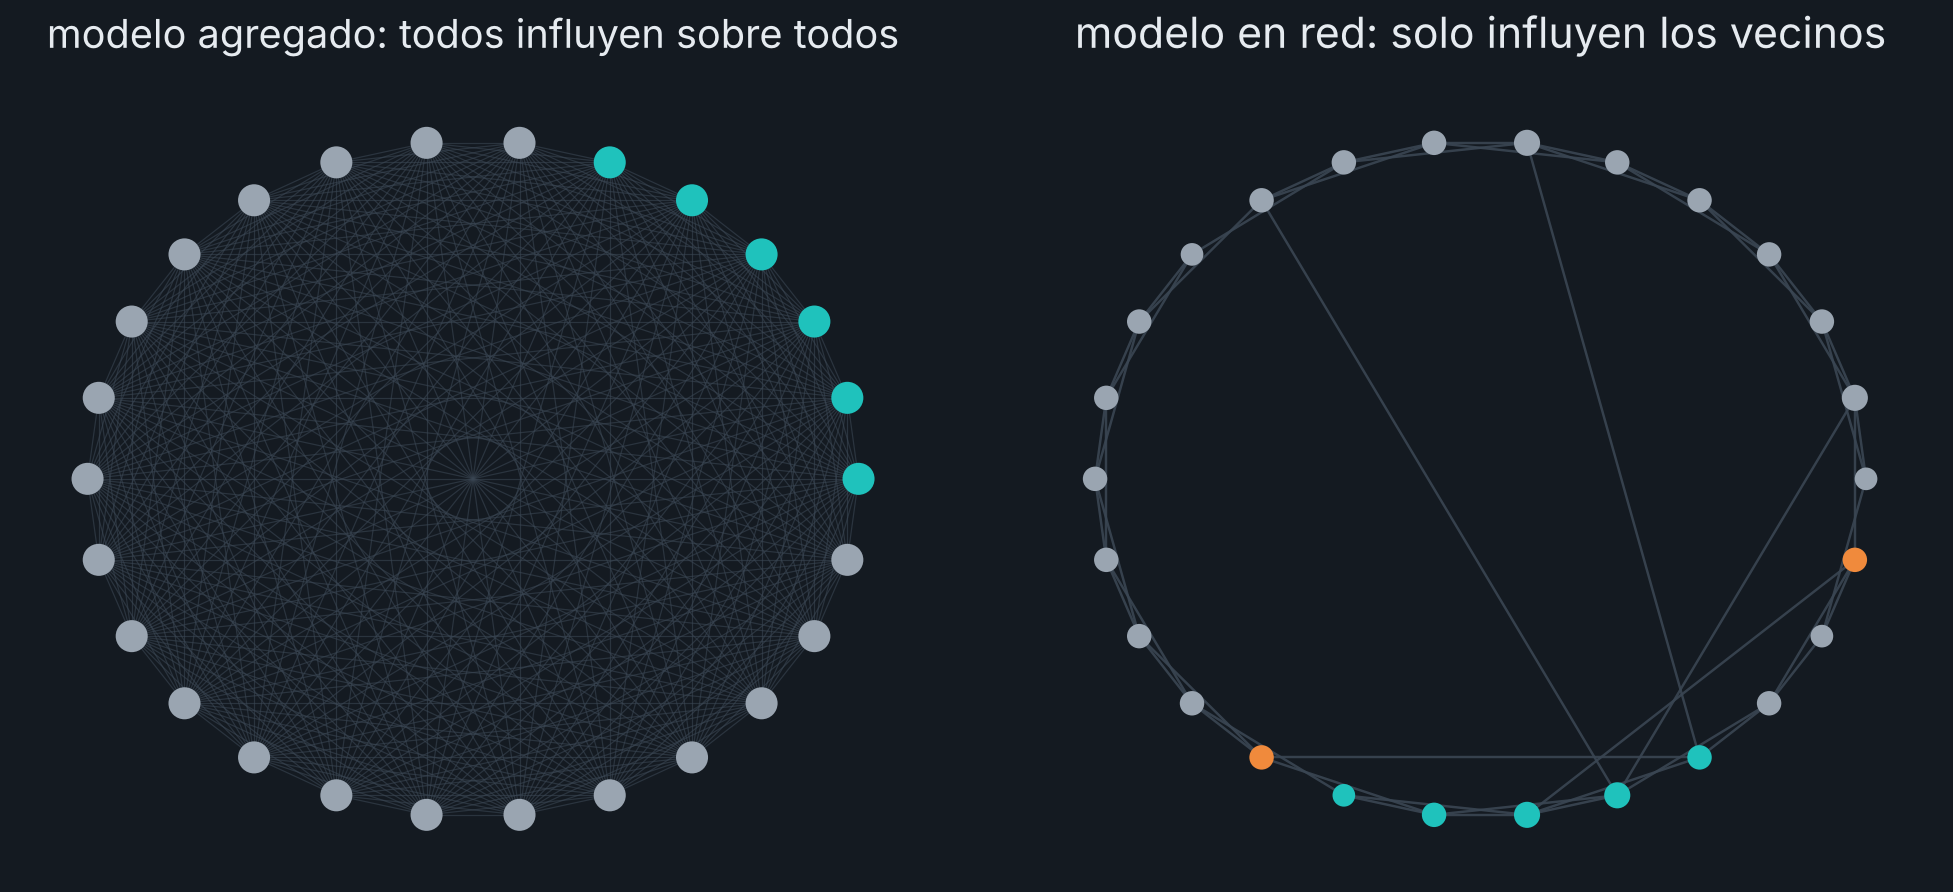
\includegraphics[width=\linewidth]{mezcla_vs_red.png}
    \end{column}
    \begin{column}{0.44\textwidth}
      \raggedright
      Bass: todos influyen sobre todos. En la realidad, solo los contactos.\par\vskip3mm
      \begin{itemize}
        \item ¿Qué pasa sin publicidad?
        \item ¿Importa la densidad o la forma de la red?
        \item ¿Cuánto se pierde con una campaña corta?
        \item ¿Responden igual una consola y un videojuego?
      \end{itemize}
    \end{column}
  \end{columns}
\end{frame}
\note{\textbf{Jesus (0:50).} El modelo de Bass describe bien las curvas agregadas, pero supone que todos influyen sobre todos, como en la red de la izquierda. En la vida real la influencia viaja por una red concreta, como la de la derecha. Eso deja cuatro preguntas sin responder: qué pasa sin publicidad, si importa la estructura de la red, cuánto se pierde con una campaña corta y si una consola y un videojuego responden igual.}

% =================================================================== 4. justificación
\renewcommand{\seccion}{Justificación}
\begin{frame}{Simular permite probar lo que no se puede observar}
  \vskip5mm
  \begin{columns}[t,totalwidth=\textwidth]
    \begin{column}{0.3\textwidth}
      {\plexmedia\color{azul}Individuos y red}\par\vskip2mm
      \nota{Cada persona es un agente con sus contactos y una regla de decisión.}
    \end{column}
    \begin{column}{0.3\textwidth}
      {\plexmedia\color{azul}Contrafactuales}\par\vskip2mm
      \nota{Lanzar sin publicidad, cambiar la red o acortar la campaña: imposible de observar en la realidad.}
    \end{column}
    \begin{column}{0.3\textwidth}
      {\plexmedia\color{azul}Datos reales}\par\vskip2mm
      \nota{PS5: calibrada y evaluada con ventas oficiales. GTA\,6, sin ventas aún: por analogía con GTA\,V.}
    \end{column}
  \end{columns}
  \vskip10mm
  \nota{NetLogo: libre, el modelo completo en un archivo y BehaviorSpace para repetir cada escenario 30 veces.}
\end{frame}
\note{\textbf{Jesus (0:50).} La simulación basada en agentes responde esas preguntas porque representa a cada persona y sus contactos, y permite correr escenarios que no se pueden observar, como lanzar sin publicidad. Para que no fuera un ejercicio solo cualitativo, la PS5 se calibró con las ventas oficiales de Sony y se evaluó con datos que no usamos para ajustar. GTA\,6 todavía no tiene ventas, así que sus parámetros salen por analogía con GTA\,V, que es la práctica estándar antes de un lanzamiento.}

% =================================================================== 5. objetivos
\renewcommand{\seccion}{Objetivos}
\begin{frame}{Qué nos propusimos}
  \vskip2mm
  {\plexmedia General.} Medir el efecto de la publicidad y de la red sobre la adopción final, en la PS5 y en GTA\,6.\par\vskip5mm
  {\plexmedia Específicos}\par\vskip1mm
  \begin{enumerate}
    \item Implementar en NetLogo el modelo de Bass en red, con tres tipos de red.
    \item Calibrar con la PS5 (entrenamiento, validación, prueba) y parametrizar GTA\,6 por analogía.
    \item Evaluar con 30 réplicas publicidad, densidad, topología y duración.
    \item Verificar con una reimplementación en Python.
  \end{enumerate}
\end{frame}
\note{\textbf{Jesus (0:40).} El objetivo general es medir el efecto de la publicidad y de la red sobre la adopción final, en la PS5 y en GTA\,6. Los específicos: implementarlo en NetLogo con tres tipos de red, calibrarlo con partición entrenamiento-validación-prueba, evaluar los escenarios con réplicas y verificarlo con una reimplementación independiente en Python.}

% =================================================================== 6. modelo
\renewcommand{\seccion}{Metodología}
\begin{frame}{Cada mes, cada persona decide: publicidad y vecinos}
  \vskip4mm
  \begin{center}{\Large $P_i = 1 - (1 - \textcolor{terracota}{p\,a_t})\,(1 - \textcolor{azul}{q\,f_i})$}\end{center}
  \vskip5mm
  \begin{columns}[T,totalwidth=\textwidth]
    \begin{column}{0.46\textwidth}
      {\color{terracota}\plexmedia publicidad}\par\nota{$p$: probabilidad mensual de que la campaña convenza; $a_t=1$ mientras está activa.}\par\vskip3mm
      {\color{azul}\plexmedia imitación}\par\nota{$q$ por $f_i$, la fracción de vecinos que ya adoptó.}
    \end{column}
    \begin{column}{0.48\textwidth}
      \vskip-\topsep
      {\small\begin{itemize}
        \item Adoptar es irreversible; todos deciden a la vez.
        \item Red completa = Bass: la diferencia es el efecto de la red.
        \item Redes aleatoria, mundo pequeño y libre de escala.
      \end{itemize}}
    \end{column}
  \end{columns}
\end{frame}
\note{\textbf{Jesus (1:00).} Cada agente es un nodo. Cada mes, quien no ha adoptado lo hace con esta probabilidad: la publicidad lo convence con probabilidad $p$ mientras la campaña esté activa, y sus vecinos con $q$ por la fracción de vecinos que ya adoptaron. Las decisiones se aplican todas a la vez al cerrar el mes y la adopción es irreversible. Si la red fuera completa, el modelo recuperaría la curva de Bass; la diferencia entre ambas es el efecto de la red. Usamos tres redes: aleatoria, mundo pequeño, con grupos cerrados, y libre de escala, con pocos nodos muy conectados. \emph{Le paso la palabra a David.}}

% =================================================================== 7. esquema
\begin{frame}{Del dato al escenario}
  \vskip2mm
  \begin{center}
  \begin{tikzpicture}[
    font=\small, text=tinta,
    caja/.style={draw=borde, line width=0.5pt, rounded corners=2pt, fill=white, align=center, inner sep=2pt,
                 minimum height=12mm, text width=21mm},
    etapa/.style={caja, fill=claro},
    flecha/.style={-{Latex[length=2mm]}, line width=0.8pt, draw=tinta},
    detalle/.style={font=\scriptsize, text=secundario}]
    \node[etapa] (d) at (0,0) {\plexmedia Datos\\[-1pt]{\scriptsize\color{secundario}Sony, Take-Two}};
    \node[etapa] (c) at (2.78,0) {\plexmedia Calibración\\[-1pt]{\scriptsize\color{secundario}Bass, analogía}};
    \node[etapa, fill=azulfondo, draw=azul, line width=0.8pt] (m) at (5.56,0) {\plexmedia Modelo\\[-1pt]{\scriptsize\color{secundario}NetLogo + nw}};
    \node[etapa] (e) at (8.34,0) {\plexmedia Escenarios\\[-1pt]{\scriptsize\color{secundario}BehaviorSpace}};
    \node[etapa] (a) at (11.12,0) {\plexmedia Análisis\\[-1pt]{\scriptsize\color{secundario}Python}};
    \draw[flecha] (d) -- (c); \draw[flecha] (c) -- (m);
    \draw[flecha] (m) -- (e); \draw[flecha] (e) -- (a);
    % interior del modelo
    \node[caja, fill=terracotafondo, draw=terracota, text width=27mm, minimum height=9mm] (camp) at (1.6,-2.5)
      {\plexmedia Campaña\\[-1pt]{\scriptsize $p\,a_t$}};
    \node[caja, fill=azulfondo, draw=azul, text width=27mm, minimum height=9mm] (red) at (1.6,-3.75)
      {\plexmedia Red social\\[-1pt]{\scriptsize $q\,f_i$}};
    \node[caja, fill=white, draw=azul, line width=0.8pt, text width=44mm, minimum height=21mm] (regla) at (6.3,-3.125)
      {\plexmedia Regla de adopción\\[4pt]$P_i = 1-(1-p\,a_t)(1-q\,f_i)$};
    \node[caja, text width=22mm, minimum height=12mm] (est) at (10.62,-3.125) {\plexmedia Estado\\[-1pt]{\scriptsize adopta y no vuelve atrás}};
    \draw[flecha, draw=terracota] (camp.east) -- (regla.west |- camp.east);
    \draw[flecha, draw=azul] (red.east) -- (regla.west |- red.east);
    \draw[flecha] (regla) -- (est);
    \begin{scope}[on background layer]
      \node[draw=azul, dashed, rounded corners=3pt, fit=(camp)(red)(regla)(est), inner sep=2.5mm] (int) {};
    \end{scope}
    \node[font=\scriptsize, text=azul, anchor=south west] at (int.north west) {cada mes, dentro del modelo};
    \draw[flecha, draw=azul, dashed] (m.south) -- (m.south |- int.north);
  \end{tikzpicture}
  \end{center}
\end{frame}
\note{\textbf{David (0:40).} Arriba el flujo: las ventas reales dan los parámetros, la PS5 por calibración de Bass y GTA\,6 por analogía con GTA\,V; NetLogo simula; BehaviorSpace corre los cuatro experimentos; Python calcula las medidas. Abajo, lo que pasa dentro del modelo cada mes: la campaña y la red alimentan la regla, que decide si cada persona adopta.}

% =================================================================== 8. implementación
\begin{frame}[fragile]{Implementación en NetLogo}
  \vskip1mm
  \begin{columns}[c,totalwidth=\textwidth]
    \begin{column}{0.47\textwidth}
      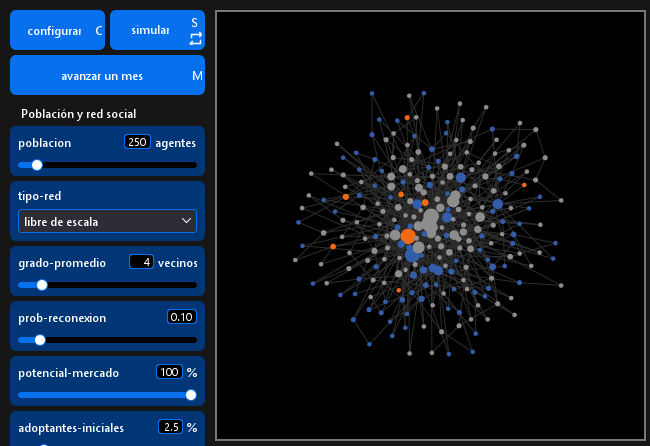
\includegraphics[width=\linewidth]{netlogo_ps5.png}\par\vskip1mm
      {\fontsize{6}{7}\selectfont\color{tenue}Interfaz del modelo (configuración de demostración: caso PS5, red libre de escala, mes 30).}
    \end{column}
    \begin{column}{0.5\textwidth}
\begin{lstlisting}
to decidir
  let p p-efectivo
  ask turtles with
      [susceptible? and not adoptante?] [
    let vecinos link-neighbors
    let f 0
    if any? vecinos [
      set f count vecinos with [adoptante?]
        / count vecinos ]
    let prob 1 - (1 - p) * (1 - q-imitacion * f)
    set decide-adoptar? random-float 1 < prob ]
end
\end{lstlisting}
      \vskip4mm
      \nota{\texttt{actualizar} aplica todas las decisiones a la vez. La extensión nw genera las redes; el selector de caso carga PS5, GTA\,6 o libre.}
    \end{column}
  \end{columns}
\end{frame}
\note{\textbf{David (0:50).} Esto es NetLogo con la extensión nw. A la izquierda, la interfaz con el caso PS5 en una red libre de escala: en azul los que ya adoptaron, en naranja los de este mes, y los nodos grandes son los más conectados. A la derecha, el procedimiento decidir: cada no adoptante cuenta qué fracción de sus vecinos ya adoptó y sortea su decisión con la fórmula. Un procedimiento aparte, actualizar, aplica todas las decisiones a la vez para que el orden de los agentes no afecte el resultado. El selector de caso carga los parámetros de la PS5 o de GTA\,6 con un clic.}

% =================================================================== 9. datos PS5
\renewcommand{\seccion}{Conjunto de datos}
\begin{frame}{La PS5: \cifraTrimestres\ trimestres de ventas oficiales de Sony}
  \begin{columns}[c,totalwidth=\textwidth]
    \begin{column}{0.6\textwidth}
      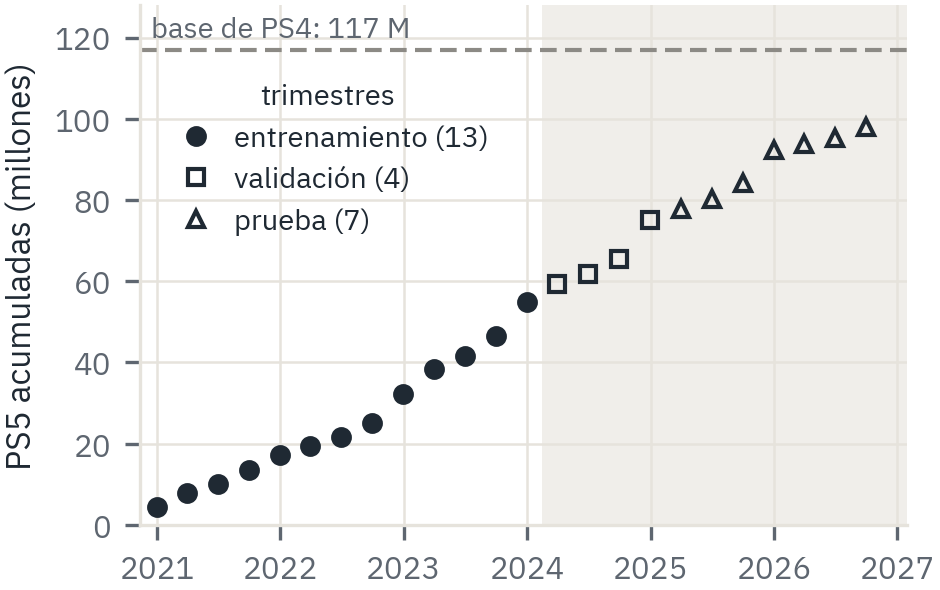
\includegraphics[width=\linewidth]{serie_ps5.png}
    \end{column}
    \begin{column}{0.36\textwidth}
      {\small\begin{itemize}
        \item \cifraPsUnidadesIni\ a \cifraPsUnidadesFin\ millones acumulados, dic.\,2020 a sep.\,2026.
        \item Adopción = acumulado / base de PS4 (\cifraUniverso\,M), fijada antes de ver la prueba.
        \item Simulación: \cifraCorridas\ corridas de 1000 agentes.
      \end{itemize}}
    \end{column}
  \end{columns}
  \fuente{Sony Interactive Entertainment, Business Data \& Sales (unidades vendidas a tiendas).}
\end{frame}
\note{\textbf{David (0:40).} La serie real son las unidades de PS5 que Sony publica cada trimestre: \cifraTrimestres\ trimestres, de \cifraPsUnidadesIni\ a \cifraPsUnidadesFin\ millones. La expresamos como porcentaje de la base de la PS4, \cifraUniverso\ millones, que fijamos antes de mirar los datos de prueba. El segundo conjunto lo genera la simulación: \cifraCorridas\ corridas de mil agentes.}

% =================================================================== 10. analogía GTA V
\begin{frame}{GTA\,6 aún no tiene ventas: lo parametrizamos con GTA\,V}
  \begin{columns}[c,totalwidth=\textwidth]
    \begin{column}{0.54\textwidth}
      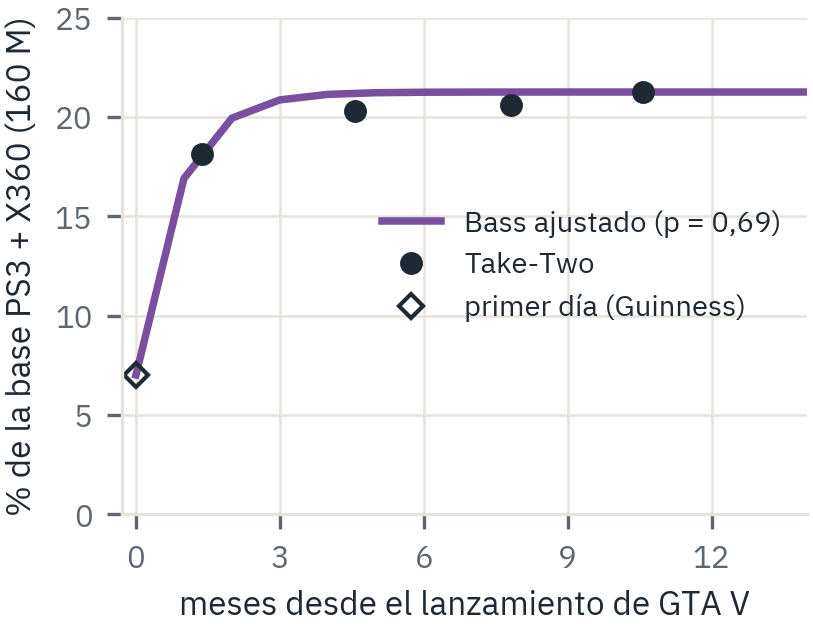
\includegraphics[width=0.94\linewidth]{analogia_gtav.png}
    \end{column}
    \begin{column}{0.42\textwidth}
      {\small\begin{itemize}
        \item GTA\,V: \cifraGtavSeisSemanas\,M en seis semanas y \cifraGtavMeseta\,M al año, sobre \cifraGtaBase\,M de consolas.
        \item Mismo ajuste de Bass: publicidad de \textcolor{terracota}{\cifraGtaP} al mes, unas \cifraGtaRazonPQ\ veces la imitación.
        \item GTA\,6 entre dueños de PS5: potencial \cifraGtaM\,\%, \cifraGtaIniciales\,\% el primer día, \cifraGtaHorizonte\ meses.
      \end{itemize}}
    \end{column}
  \end{columns}
  \fuente{Take-Two Interactive, resultados trimestrales 2013--2014; primer día: Guinness World Records (2013).}
\end{frame}
\note{\textbf{David (0:50).} GTA\,6 no tiene ventas todavía, así que usamos el método de analogía: tomamos el lanzamiento más parecido, GTA\,V. Vendió \cifraGtavSeisSemanas\ millones en seis semanas y se estabilizó en \cifraGtavMeseta\ millones, sobre \cifraGtaBase\ millones de consolas. Con la imitación fijada en la de la PS5, el ajuste atribuye el salto del lanzamiento a la publicidad: \cifraGtaP\ al mes, unas \cifraGtaRazonPQ\ veces la imitación, lo contrario de la PS5. Así modelamos GTA\,6 entre los dueños de PS5, con un potencial del \cifraGtaM\,\% y dos años de horizonte.}

% =================================================================== 11. diseño experimental
\renewcommand{\seccion}{Diseño experimental}
\begin{frame}{Cuatro experimentos, 30 réplicas por escenario}
  \vskip2mm
  \begin{tikzpicture}[x=1mm, y=1mm, font=\scriptsize]
    \fill[azul] (0,0) rectangle (60,10);
    \fill[azulclaro] (61,0) rectangle (92,10);
    \fill[terracota] (93,0) rectangle (134,10);
    \node[text=white, align=center] at (30,5) {entrenamiento\\dic.\,2020--dic.\,2023 · \cifraObsEnt\ trimestres};
    \node[text=tinta, align=center] at (76.5,5) {validación\\2024 · \cifraObsVal\ trimestres};
    \node[text=white, align=center] at (113.5,5) {prueba\\2025--2026 · \cifraObsPru\ trimestres};
    \node[text=secundario] at (30,-3) {ajusta $p$ y $q$};
    \node[text=secundario] at (76.5,-3) {elige $m$ y la red};
    \node[text=secundario] at (113.5,-3) {solo evalúa};
  \end{tikzpicture}
  \vskip6mm
  {\footnotesize
  \begin{tabular}{@{}lp{0.74\textwidth}r@{}}
    \toprule
    & factores (E1 a E3 para ambos casos: PS5 y GTA\,6) & corridas\\
    \midrule
    E1 & publicidad \{sin, con\} $\times$ densidad $k$ = 2, 4, 6, 8, 12, 16 & 720\\
    E2 & publicidad $\times$ topología \{aleatoria, mundo pequeño, libre de escala\} & 360\\
    E3 & duración de la campaña \{0, 1, 3, 6, 12, 24 meses, permanente\} & 420\\
    E4 & calibración PS5: 3 topologías $\times$ $k$ = 4, 8, 16 & 270\\
    \bottomrule
  \end{tabular}}
\end{frame}
\note{\textbf{David (0:50).} La serie de la PS5 se parte en el tiempo: con entrenamiento estimamos $p$ y $q$; como el potencial no se puede estimar en plena fase de crecimiento, lo elegimos en validación, igual que la red; la prueba solo evalúa. Corremos cuatro experimentos, los tres de escenarios para los dos casos: publicidad por densidad, publicidad por topología y duración de la campaña, más la calibración. Cada combinación se repite 30 veces. \emph{Duvan presenta las medidas y los resultados.}}

% =================================================================== 12. medidas
\renewcommand{\seccion}{Medidas de desempeño}
\begin{frame}{Cómo medimos}
  \vskip4mm
  \begin{columns}[T,totalwidth=\textwidth]
    \begin{column}{0.47\textwidth}
      {\plexmedia\color{azul}Escenarios}\par\vskip1mm
      {\small\begin{itemize}
        \item \alert{Adopción final}: \% de la población que adoptó al final del período (PS5: \cifraHorizontePs\ meses; GTA\,6: \cifraHorizonteGta).
        \item Mes del 50\,\% y mes del pico de compras.
        \item Media e IC del 95\,\% con 30 réplicas.
      \end{itemize}}
    \end{column}
    \begin{column}{0.47\textwidth}
      {\plexmedia\color{azul}Ajuste a la serie real}\par\vskip1mm
      {\small\begin{itemize}
        \item RMSE: raíz del error cuadrático medio, en puntos porcentuales.
        \item MAPE: error porcentual absoluto medio.
        \item Por partición: entrenamiento, validación y prueba.
      \end{itemize}}
    \end{column}
  \end{columns}
\end{frame}
\note{\textbf{Duvan (0:30).} La medida principal, la que pide el enunciado, es el porcentaje de adopción al final del período: seis años para la PS5 y dos para GTA\,6. La complementamos con el mes del 50\,\% y el mes del pico de compras. Frente a la serie real usamos RMSE y MAPE por partición. Todo con 30 réplicas e intervalos del 95\,\%.}

% =================================================================== 13. calibración
\renewcommand{\seccion}{Resultados}
\begin{frame}{El modelo sigue la serie de prueba de la PS5}
  \begin{columns}[c,totalwidth=\textwidth]
    \begin{column}{0.64\textwidth}
      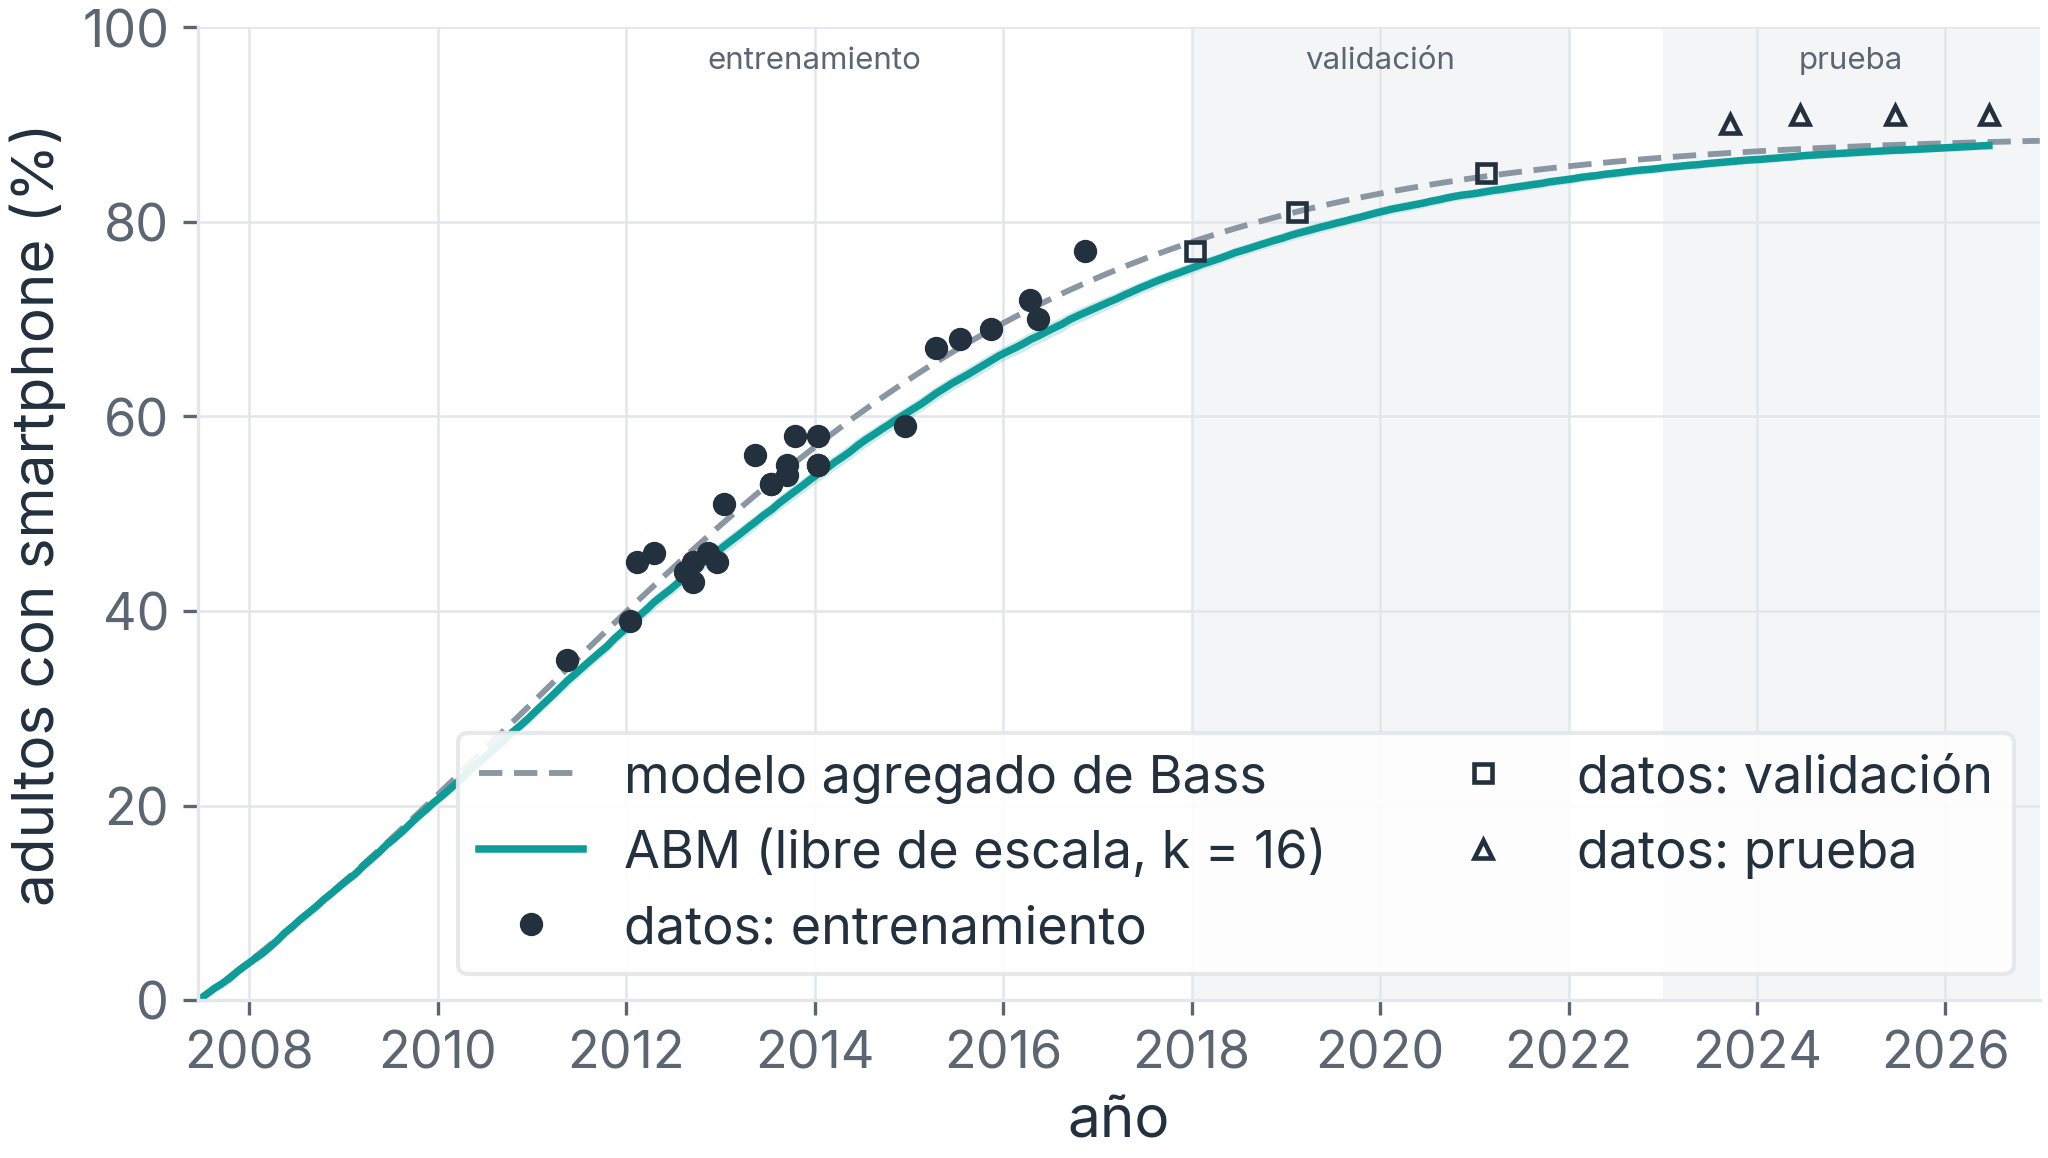
\includegraphics[width=\linewidth]{fig_calibracion.png}
    \end{column}
    \begin{column}{0.32\textwidth}
      \cifra{\cifraAbmRmsePru\ pp}{error en prueba del modelo de agentes (Bass: \cifraBassRmsePru)}\par\vskip5mm
      \nota{Bass anual: $p$\,=\,\cifraBassP, $q$\,=\,\cifraBassQ; la imitación pesa \cifraBassRazonQP\ veces más. Red elegida en validación: \cifraAbmSelRedNombre, $k$\,=\,\cifraAbmSelK.}
    \end{column}
  \end{columns}
\end{frame}
\note{\textbf{Duvan (0:50).} El ajuste da $p$ = \cifraBassP\ y $q$ = \cifraBassQ\ anuales: en la PS5 la imitación pesa \cifraBassRazonQP\ veces más que la publicidad. En validación se eligió la \cifraAbmSelRedNombre\ con $k$ = \cifraAbmSelK. En prueba, que nunca usamos para ajustar, el error es de \cifraAbmRmsePru\ puntos, mayor que el de Bass, \cifraBassRmsePru, porque la red frena la difusión. Ambos quedan un poco por debajo del dato de Sony de noviembre de 2026, más de 100 millones: la PS5 probablemente superará la base de la PS4.}

% =================================================================== 14. publicidad
\begin{frame}{Sin publicidad, ninguno de los dos llega lejos}
  \vskip1mm
  \begin{center}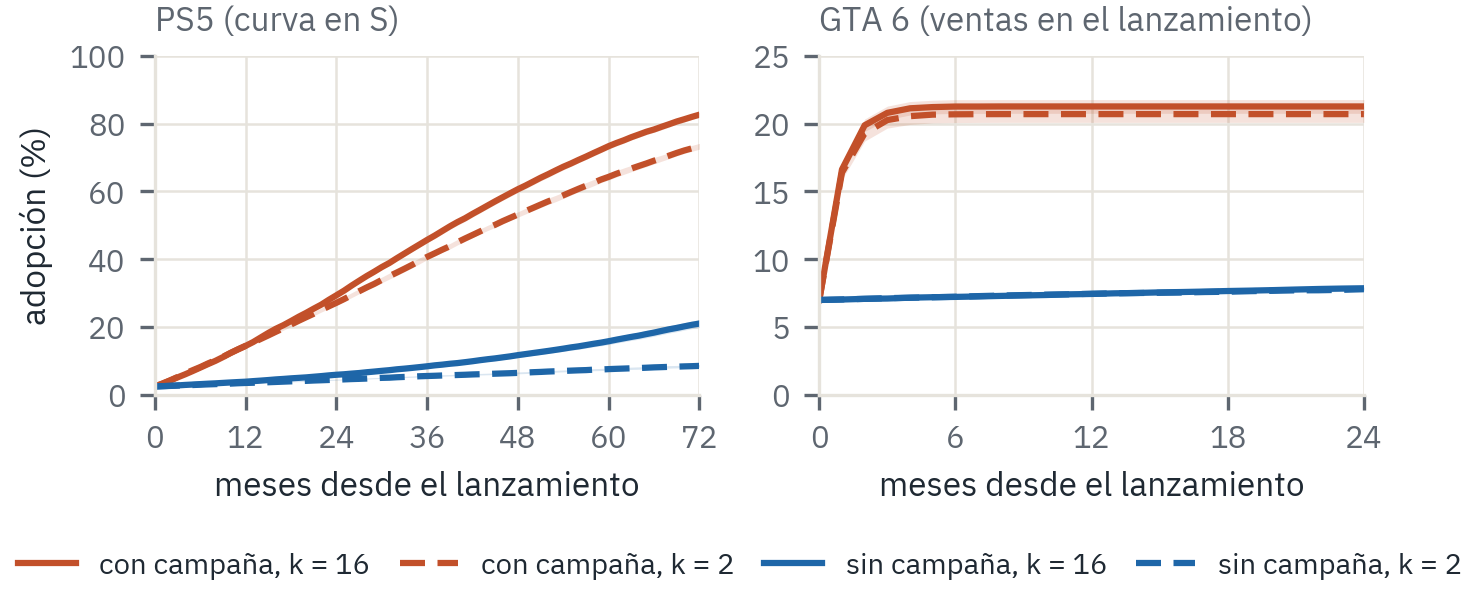
\includegraphics[width=0.9\linewidth]{publicidad_casos.png}\end{center}
  \vskip-3mm
  \nota{Red de mundo pequeño con $k$\,=\,2 (discontinua) y 16 (continua).}
\end{frame}
\note{\textbf{Duvan (0:50).} El resultado central. En la PS5, sin publicidad la adopción queda entre el \cifraPsSinMin\ y el \cifraPsSinMax\,\% en seis años; con campaña, entre el \cifraPsConMin\ y el \cifraPsConMax\,\%, con la curva en S. En GTA\,6 la campaña lo decide todo: con ella se alcanza el potencial casi en el primer mes; sin ella la adopción apenas pasa de los compradores del primer día. Sin publicidad, la PS5 simplemente no despega.}

% =================================================================== 15. densidad y topología
\begin{frame}{La red pesa sobre todo cuando no hay publicidad}
  \begin{columns}[c,totalwidth=\textwidth]
    \begin{column}{0.66\textwidth}
      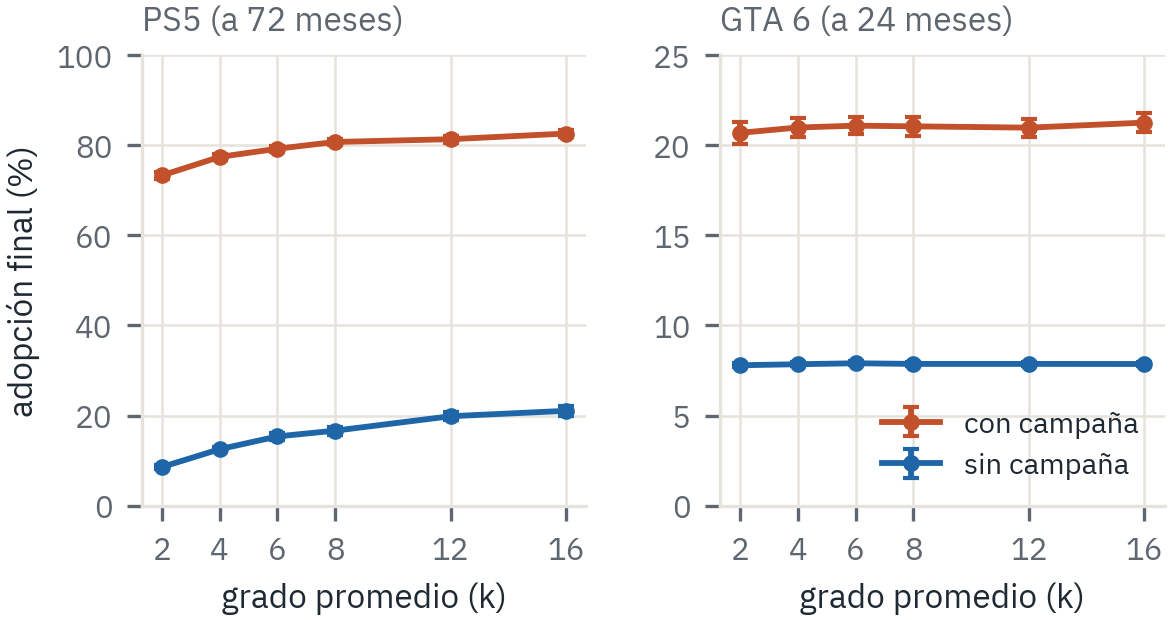
\includegraphics[width=\linewidth]{densidad.png}
    \end{column}
    \begin{column}{0.3\textwidth}
      \cifra{×\,\cifraPsSinRazon}{adopción de la PS5 sin campaña al pasar de $k$\,=\,2 a 16}\par\vskip4mm
      \nota{Con campaña, la misma diferencia solo la multiplica por \cifraPsConRazon. Sin campaña, la red de mundo pequeño es la topología más lenta.}
    \end{column}
  \end{columns}
\end{frame}
\note{\textbf{Duvan (0:50).} En la PS5 sin publicidad, pasar de 2 a 16 contactos multiplica la adopción por \cifraPsSinRazon; con campaña solo por \cifraPsConRazon, porque la publicidad siembra adoptantes en toda la red. En la topología pasa lo mismo: sin campaña, la red de mundo pequeño es la más lenta de las tres, porque sus grupos cerrados atrapan la influencia, y la libre de escala la más variable, porque depende de si un nodo muy conectado adopta temprano. En GTA\,6 la red casi no cambia nada.}

% =================================================================== 16. duración
\begin{frame}{GTA\,6: basta un mes; PS5: la campaña necesita tiempo}
  \begin{columns}[c,totalwidth=\textwidth]
    \begin{column}{0.58\textwidth}
      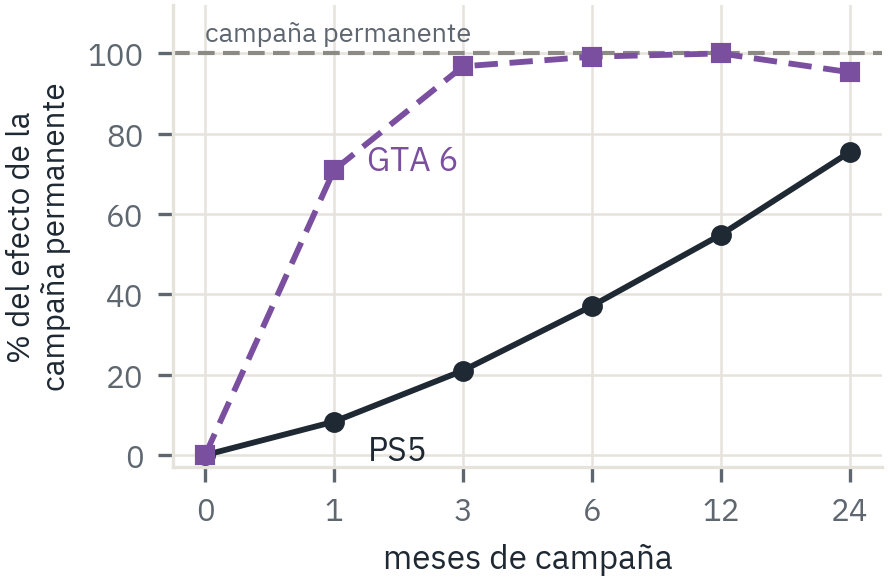
\includegraphics[width=\linewidth]{fraccion_duracion.png}
    \end{column}
    \begin{column}{0.38\textwidth}
      \cifra{\cifraFraccionGtaDUno\,\%}{del efecto de una campaña permanente se logra con un mes en GTA\,6}\par\vskip5mm
      \cifra{\cifraFraccionPsDDoce\,\%}{se logra con un año en la PS5 (dos años: \cifraFraccionPsDVeinticuatro\,\%)}
    \end{column}
  \end{columns}
\end{frame}
\note{\textbf{Duvan (0:40).} Si la campaña se corta, ¿cuánto se pierde? En GTA\,6, un solo mes ya logra el \cifraFraccionGtaDUno\,\% del efecto de una campaña permanente: el lanzamiento concentra casi todo. En la PS5 el rendimiento es gradual: un año logra el \cifraFraccionPsDDoce\,\% y dos años el \cifraFraccionPsDVeinticuatro\,\%, porque la imitación necesita tiempo para sostener la difusión. Los puntos de GTA\,6 que pasan apenas del 100\,\% son variación entre réplicas. \emph{David hace la demostración.}}

% =================================================================== 17. demo
\renewcommand{\seccion}{Demostración}
\begin{frame}{En vivo en NetLogo}
  \vskip1mm
  \begin{columns}[c,totalwidth=\textwidth]
    \begin{column}{0.4\textwidth}
      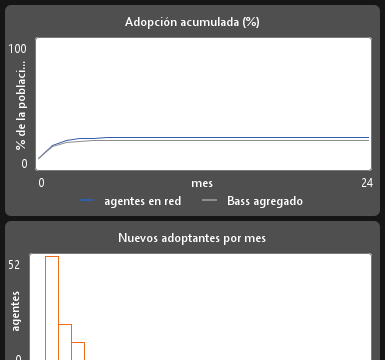
\includegraphics[width=0.86\linewidth]{netlogo_gta6.png}\par\vskip1mm
      {\fontsize{6}{7}\selectfont\color{tenue}Caso GTA\,6: compras concentradas en el primer mes.}
    \end{column}
    \begin{column}{0.56\textwidth}
      {\small\begin{enumerate}
        \item Caso \alert{GTA\,6} $\to$ configurar $\to$ simular: el pico llega en el primer mes.
        \item Campaña apagada: la adopción apenas pasa del \cifraGtaIniciales\,\%.
        \item Caso \textcolor{azul}{PS5}: curva en S frente a la de Bass.
      \end{enumerate}}
      \vskip2mm
      \nota{Si sobra tiempo: PS5 sin campaña y $k$ de 16 a 2; Herramientas $\to$ BehaviorSpace.}
    \end{column}
  \end{columns}
\end{frame}
\note{\textbf{David (1:10).} Demostración en vivo; los pasos están en el guion. Hacer 1 a 3; los otros dos solo si sobra tiempo.}

% =================================================================== 18. conclusiones
\renewcommand{\seccion}{Conclusiones}
\begin{frame}{Publicidad primero, red después}
  \vskip2mm
  \begin{enumerate}
    \item PS5: sin campaña, a lo sumo \cifraPsSinMaxGlobal\,\%; con campaña, al menos \cifraPsConMin\,\%.
    \item GTA\,6: un mes de campaña logra el \cifraFraccionGtaDUno\,\% del efecto.
    \item La red pesa sobre todo cuando no hay publicidad.
    \item Error en prueba: \cifraAbmRmsePru\ pp; la reimplementación en Python coincide.
  \end{enumerate}
  \vskip5mm
  \nota{Limitaciones: coeficientes iguales para todos, red fija, unidades vendidas a tiendas y parámetros de GTA\,6 hipotéticos.}
\end{frame}
\note{\textbf{Duvan (0:30).} Cuatro conclusiones. En la PS5, la publicidad es la condición del despegue. En GTA\,6, el primer mes de campaña decide el resultado. La red pesa sobre todo cuando no hay publicidad. Y el modelo quedó validado con datos que no usamos para ajustar y verificado con una reimplementación independiente.}

% =================================================================== 19. referencias
\renewcommand{\seccion}{Referencias}
\begin{frame}{Fuentes}
  \vskip0.5mm
  \raggedright\fontsize{8}{9.6}\selectfont
  \setlength{\parskip}{1.1mm}
  \referencia{Bass, F.\,M. (1969). A new product growth model for consumer durables. \textit{Management Science}, 15(5), 215--227.}
  \referencia{Goldenberg, J., Libai, B. y Muller, E. (2001). Talk of the network. \textit{Marketing Letters}, 12(3), 211--223.}
  \referencia{Rogers, E.\,M. (2003). \textit{Diffusion of Innovations} (5.ª ed.). Free Press.}
  \referencia{Thomas, R.\,J. (1985). Estimating market growth for new products: an analogical diffusion model approach. \textit{Journal of Product Innovation Management}, 2(1), 45--55.}
  \referencia{Watts, D.\,J. y Strogatz, S.\,H. (1998). Collective dynamics of `small-world' networks. \textit{Nature}, 393, 440--442.}
  \referencia{Wilensky, U. (1999). NetLogo. Northwestern University.}
  \referencia{Sony Interactive Entertainment (2026). Business Data \& Sales.}
  \referencia{Take-Two Interactive (2013--2014). Resultados trimestrales, años fiscales 2014 y 2015.}
  \referencia{Guinness World Records (2013, 2023). Récords de ventas de GTA\,V y de vistas del tráiler de GTA\,6.}
\end{frame}
\note{\textbf{Duvan (0:10).} Las referencias están en pantalla. Gracias; quedamos atentos a sus preguntas.}

\end{document}
"  -> notas del orador
% Las cifras salen de ../articulo/tablas/cifras.tex (analisis/analisis_resultados.py) y las
% figuras de ../analisis/figuras/diapositivas (analisis/figuras_diapositivas.py).
\ifdefined\connotas
  \documentclass[aspectratio=169,11pt,notes=only]{beamer}
\else
  \documentclass[aspectratio=169,11pt]{beamer}
\fi

\usepackage{fontspec}
\usepackage[spanish,es-noshorthands]{babel}
\usepackage{booktabs}
\usepackage{tikz}
\usepackage{listings}
\usetikzlibrary{arrows.meta,positioning,calc,fit,backgrounds}

% ------------------------------------------------------------------ tipografía
\setsansfont{IBMPlexSans}[Path=../analisis/fuentes/, Extension=.ttf, UprightFont=*-Regular,
  BoldFont=*-SemiBold, ItalicFont=*-Regular, ItalicFeatures={FakeSlant=0.18}]
\newfontfamily\plexmedia{IBMPlexSans-Medium}[Path=../analisis/fuentes/, Extension=.ttf]
\usefonttheme{professionalfonts}
\usefonttheme[onlymath]{serif}
\hyphenpenalty=10000
\exhyphenpenalty=10000

% ------------------------------------------------------------------ colores
% terracota = publicidad (con campaña), azul = imitación (sin campaña), igual que en el modelo y las figuras
\definecolor{papel}{HTML}{FBFAF6}
\definecolor{tinta}{HTML}{1F2933}
\definecolor{secundario}{HTML}{5E6670}
\definecolor{tenue}{HTML}{8C8A85}
\definecolor{borde}{HTML}{B9B4AA}
\definecolor{claro}{HTML}{F1EEE7}
\definecolor{azul}{HTML}{1E66A8}
\definecolor{azulclaro}{HTML}{8DB3D6}
\definecolor{azulfondo}{HTML}{E4EDF6}
\definecolor{terracota}{HTML}{C2502A}
\definecolor{terracotafondo}{HTML}{F7E6DE}

\setbeamercolor{background canvas}{bg=papel}
\setbeamercolor{normal text}{fg=tinta}
\setbeamercolor{structure}{fg=azul}
\setbeamercolor{frametitle}{fg=tinta}
\setbeamercolor{alerted text}{fg=terracota}
\setbeamercolor{item}{fg=terracota}
\setbeamercolor{enumerate item}{fg=terracota}

% ------------------------------------------------------------------ plantillas
\setbeamertemplate{navigation symbols}{}
\setbeamersize{text margin left=13mm, text margin right=13mm}
\setbeamerfont{frametitle}{size=\Large}
\newcommand{\seccion}{}
\setbeamertemplate{frametitle}{%
  \vskip6mm%
  {\scriptsize\addfontfeatures{LetterSpace=12}\color{terracota}\MakeUppercase{\seccion}}\par\vskip1mm%
  {\usebeamerfont{frametitle}\plexmedia\color{tinta}\insertframetitle\par}\vskip0.5mm}
\setbeamertemplate{footline}{%
  \hbox to \paperwidth{\hskip13mm{\fontsize{6}{7}\selectfont\color{tenue}Delgado · Monroy · Baquero\quad Universidad de los Llanos}%
  \hfill{\fontsize{6}{7}\selectfont\color{tenue}\insertframenumber\,/\,\inserttotalframenumber}\hskip13mm}\vskip4mm}
\setbeamertemplate{itemize item}{\raisebox{0.3ex}{\color{terracota}\rule{0.8ex}{0.8ex}}}
\setbeamertemplate{enumerate item}{\color{terracota}\plexmedia\insertenumlabel.}
\setbeamertemplate{itemize/enumerate body begin}{\raggedright}
\setlength{\leftmargini}{1.3em}
\setbeamertemplate{note page}{\vskip5mm\hskip6mm\begin{minipage}[t]{0.42\paperwidth}\vskip0pt\insertslideintonotes{0.4}\end{minipage}%
  \hskip4mm\begin{minipage}[t]{0.4\paperwidth}\vskip0pt\raggedright\footnotesize
  {\scriptsize\color{terracota}DIAPOSITIVA \insertframenumber}\par\vskip2mm\insertnote\end{minipage}}

\lstset{basicstyle=\ttfamily\fontsize{7.2}{8.6}\selectfont\color{tinta}, keywordstyle=\color{azul}, columns=fullflexible,
  keepspaces=true, frame=none, aboveskip=0pt, belowskip=0pt,
  morekeywords={to,end,ask,let,set,if,with,count,any?,random-float,turtles,link-neighbors,not}}

% ------------------------------------------------------------------ utilidades
\newcommand{\cifra}[2]{% número grande + leyenda
  \begin{minipage}[t]{\linewidth}\raggedright{\plexmedia\fontsize{24}{26}\selectfont\color{azul}#1\par}\vskip1mm
  {\small\color{secundario}#2\par}\end{minipage}}
\newcommand{\nota}[1]{{\raggedright\footnotesize\color{secundario}#1\par}}
\newcommand{\fuente}[1]{\par\vfill{\fontsize{6}{7}\selectfont\color{tenue}#1}\par\vskip1mm}
\newcommand{\referencia}[1]{\par\hangindent=1.4em\hangafter=1 #1\par}

% generado por analisis_resultados.py
\newcommand{\cifraBassP}{0,079}
\newcommand{\cifraBassQ}{0,242}
\newcommand{\cifraBassM}{89}
\newcommand{\cifraBassPmes}{0,0066}
\newcommand{\cifraBassQmes}{0,0202}
\newcommand{\cifraBassPico}{3,5}
\newcommand{\cifraBassRmseEnt}{2,29}
\newcommand{\cifraBassMapeEnt}{3,64}
\newcommand{\cifraBassRmseVal}{0,63}
\newcommand{\cifraBassMapeVal}{0,60}
\newcommand{\cifraBassRmsePru}{3,10}
\newcommand{\cifraBassMapePru}{3,40}
\newcommand{\cifraAbmSelRed}{libre de escala}
\newcommand{\cifraAbmSelK}{16}
\newcommand{\cifraAbmRmseEnt}{3,52}
\newcommand{\cifraAbmRmseVal}{1,93}
\newcommand{\cifraAbmRmsePru}{3,74}
\newcommand{\cifraAbmMapePru}{4,10}
\newcommand{\cifraAbmFinal}{87,8}
\newcommand{\cifraAbmRmseValMax}{4,90}
\newcommand{\cifraAbmRmsePruMax}{5,37}
\newcommand{\cifraAbmPeorRed}{aleatoria}
\newcommand{\cifraAbmPeorK}{4}
\newcommand{\cifraSinCalKDos}{8,1}
\newcommand{\cifraSinCalKDosIc}{0,3}
\newcommand{\cifraTcincuentaSinCalKDos}{--}
\newcommand{\cifraSinCalKCuatro}{11,2}
\newcommand{\cifraSinCalKCuatroIc}{0,5}
\newcommand{\cifraTcincuentaSinCalKCuatro}{--}
\newcommand{\cifraSinCalKSeis}{13,2}
\newcommand{\cifraSinCalKSeisIc}{0,7}
\newcommand{\cifraTcincuentaSinCalKSeis}{--}
\newcommand{\cifraSinCalKOcho}{14,9}
\newcommand{\cifraSinCalKOchoIc}{0,8}
\newcommand{\cifraTcincuentaSinCalKOcho}{--}
\newcommand{\cifraSinCalKDoce}{15,1}
\newcommand{\cifraSinCalKDoceIc}{0,8}
\newcommand{\cifraTcincuentaSinCalKDoce}{--}
\newcommand{\cifraSinCalKDieciseis}{16,9}
\newcommand{\cifraSinCalKDieciseisIc}{1,0}
\newcommand{\cifraTcincuentaSinCalKDieciseis}{--}
\newcommand{\cifraConCalKDos}{79,8}
\newcommand{\cifraConCalKDosIc}{0,6}
\newcommand{\cifraTcincuentaConCalKDos}{63}
\newcommand{\cifraConCalKCuatro}{82,9}
\newcommand{\cifraConCalKCuatroIc}{0,5}
\newcommand{\cifraTcincuentaConCalKCuatro}{62}
\newcommand{\cifraConCalKSeis}{83,8}
\newcommand{\cifraConCalKSeisIc}{0,6}
\newcommand{\cifraTcincuentaConCalKSeis}{59}
\newcommand{\cifraConCalKOcho}{84,4}
\newcommand{\cifraConCalKOchoIc}{0,6}
\newcommand{\cifraTcincuentaConCalKOcho}{59}
\newcommand{\cifraConCalKDoce}{85,5}
\newcommand{\cifraConCalKDoceIc}{0,5}
\newcommand{\cifraTcincuentaConCalKDoce}{58}
\newcommand{\cifraConCalKDieciseis}{85,4}
\newcommand{\cifraConCalKDieciseisIc}{0,6}
\newcommand{\cifraTcincuentaConCalKDieciseis}{59}
\newcommand{\cifraSinLitKDos}{11,8}
\newcommand{\cifraSinLitKDosIc}{0,5}
\newcommand{\cifraTcincuentaSinLitKDos}{--}
\newcommand{\cifraSinLitKCuatro}{18,9}
\newcommand{\cifraSinLitKCuatroIc}{0,7}
\newcommand{\cifraTcincuentaSinLitKCuatro}{--}
\newcommand{\cifraSinLitKSeis}{24,2}
\newcommand{\cifraSinLitKSeisIc}{0,8}
\newcommand{\cifraTcincuentaSinLitKSeis}{--}
\newcommand{\cifraSinLitKOcho}{27,0}
\newcommand{\cifraSinLitKOchoIc}{1,1}
\newcommand{\cifraTcincuentaSinLitKOcho}{--}
\newcommand{\cifraSinLitKDoce}{35,0}
\newcommand{\cifraSinLitKDoceIc}{1,2}
\newcommand{\cifraTcincuentaSinLitKDoce}{--}
\newcommand{\cifraSinLitKDieciseis}{35,9}
\newcommand{\cifraSinLitKDieciseisIc}{1,5}
\newcommand{\cifraTcincuentaSinLitKDieciseis}{--}
\newcommand{\cifraConLitKDos}{87,7}
\newcommand{\cifraConLitKDosIc}{0,6}
\newcommand{\cifraTcincuentaConLitKDos}{54}
\newcommand{\cifraConLitKCuatro}{91,3}
\newcommand{\cifraConLitKCuatroIc}{0,4}
\newcommand{\cifraTcincuentaConLitKCuatro}{52}
\newcommand{\cifraConLitKSeis}{93,2}
\newcommand{\cifraConLitKSeisIc}{0,4}
\newcommand{\cifraTcincuentaConLitKSeis}{48}
\newcommand{\cifraConLitKOcho}{93,8}
\newcommand{\cifraConLitKOchoIc}{0,3}
\newcommand{\cifraTcincuentaConLitKOcho}{48}
\newcommand{\cifraConLitKDoce}{94,0}
\newcommand{\cifraConLitKDoceIc}{0,3}
\newcommand{\cifraTcincuentaConLitKDoce}{48}
\newcommand{\cifraConLitKDieciseis}{94,2}
\newcommand{\cifraConLitKDieciseisIc}{0,4}
\newcommand{\cifraTcincuentaConLitKDieciseis}{48}
\newcommand{\cifraDensidadGananciaCon}{6}
\newcommand{\cifraDensidadRazonSinCal}{2,1}
\newcommand{\cifraDensidadRazonSinLit}{3,0}
\newcommand{\cifraTopoSinCalAleatoria}{15,4}
\newcommand{\cifraTopoSinCalAleatoriaIc}{0,9}
\newcommand{\cifraTopoSinCalAleatoriaDe}{2,3}
\newcommand{\cifraTopoSinCalAleatoriaProp}{0}
\newcommand{\cifraTopoSinCalEscala}{13,1}
\newcommand{\cifraTopoSinCalEscalaIc}{1,2}
\newcommand{\cifraTopoSinCalEscalaDe}{3,3}
\newcommand{\cifraTopoSinCalEscalaProp}{0}
\newcommand{\cifraTopoSinCalMundo}{12,9}
\newcommand{\cifraTopoSinCalMundoIc}{0,5}
\newcommand{\cifraTopoSinCalMundoDe}{1,4}
\newcommand{\cifraTopoSinCalMundoProp}{0}
\newcommand{\cifraTopoConCalAleatoria}{83,6}
\newcommand{\cifraTopoConCalAleatoriaIc}{0,6}
\newcommand{\cifraTopoConCalAleatoriaDe}{1,5}
\newcommand{\cifraTopoConCalAleatoriaProp}{100}
\newcommand{\cifraTopoConCalEscala}{84,5}
\newcommand{\cifraTopoConCalEscalaIc}{0,7}
\newcommand{\cifraTopoConCalEscalaDe}{1,9}
\newcommand{\cifraTopoConCalEscalaProp}{100}
\newcommand{\cifraTopoConCalMundo}{83,8}
\newcommand{\cifraTopoConCalMundoIc}{0,7}
\newcommand{\cifraTopoConCalMundoDe}{2,0}
\newcommand{\cifraTopoConCalMundoProp}{100}
\newcommand{\cifraTopoSinLitAleatoria}{33,3}
\newcommand{\cifraTopoSinLitAleatoriaIc}{2,1}
\newcommand{\cifraTopoSinLitAleatoriaDe}{5,6}
\newcommand{\cifraTopoSinLitAleatoriaProp}{0}
\newcommand{\cifraTopoSinLitEscala}{34,2}
\newcommand{\cifraTopoSinLitEscalaIc}{2,9}
\newcommand{\cifraTopoSinLitEscalaDe}{7,8}
\newcommand{\cifraTopoSinLitEscalaProp}{3}
\newcommand{\cifraTopoSinLitMundo}{23,4}
\newcommand{\cifraTopoSinLitMundoIc}{1,1}
\newcommand{\cifraTopoSinLitMundoDe}{2,8}
\newcommand{\cifraTopoSinLitMundoProp}{0}
\newcommand{\cifraTopoConLitAleatoria}{93,3}
\newcommand{\cifraTopoConLitAleatoriaIc}{0,4}
\newcommand{\cifraTopoConLitAleatoriaDe}{1,1}
\newcommand{\cifraTopoConLitAleatoriaProp}{100}
\newcommand{\cifraTopoConLitEscala}{93,3}
\newcommand{\cifraTopoConLitEscalaIc}{0,3}
\newcommand{\cifraTopoConLitEscalaDe}{0,9}
\newcommand{\cifraTopoConLitEscalaProp}{100}
\newcommand{\cifraTopoConLitMundo}{92,7}
\newcommand{\cifraTopoConLitMundoIc}{0,4}
\newcommand{\cifraTopoConLitMundoDe}{1,1}
\newcommand{\cifraTopoConLitMundoProp}{100}
\newcommand{\cifraDurCalDCero}{13,0}
\newcommand{\cifraDurCalDCeroIc}{0,7}
\newcommand{\cifraTcincuentaDurCalDCero}{--}
\newcommand{\cifraDurCalDSeis}{28,5}
\newcommand{\cifraDurCalDSeisIc}{0,9}
\newcommand{\cifraTcincuentaDurCalDSeis}{--}
\newcommand{\cifraDurCalDDoce}{41,0}
\newcommand{\cifraDurCalDDoceIc}{1,4}
\newcommand{\cifraTcincuentaDurCalDDoce}{--}
\newcommand{\cifraDurCalDVeinticuatro}{54,6}
\newcommand{\cifraDurCalDVeinticuatroIc}{1,2}
\newcommand{\cifraTcincuentaDurCalDVeinticuatro}{107}
\newcommand{\cifraDurCalDSesenta}{74,2}
\newcommand{\cifraDurCalDSesentaIc}{0,7}
\newcommand{\cifraTcincuentaDurCalDSesenta}{59}
\newcommand{\cifraDurCalDCientoveinte}{84,4}
\newcommand{\cifraDurCalDCientoveinteIc}{0,6}
\newcommand{\cifraTcincuentaDurCalDCientoveinte}{59}
\newcommand{\cifraDurLitDCero}{23,9}
\newcommand{\cifraDurLitDCeroIc}{1,1}
\newcommand{\cifraTcincuentaDurLitDCero}{--}
\newcommand{\cifraDurLitDSeis}{46,9}
\newcommand{\cifraDurLitDSeisIc}{1,9}
\newcommand{\cifraTcincuentaDurLitDSeis}{--}
\newcommand{\cifraDurLitDDoce}{60,9}
\newcommand{\cifraDurLitDDoceIc}{1,1}
\newcommand{\cifraTcincuentaDurLitDDoce}{98}
\newcommand{\cifraDurLitDVeinticuatro}{74,5}
\newcommand{\cifraDurLitDVeinticuatroIc}{1,1}
\newcommand{\cifraTcincuentaDurLitDVeinticuatro}{72}
\newcommand{\cifraDurLitDSesenta}{88,1}
\newcommand{\cifraDurLitDSesentaIc}{0,7}
\newcommand{\cifraTcincuentaDurLitDSesenta}{50}
\newcommand{\cifraDurLitDCientoveinte}{93,0}
\newcommand{\cifraDurLitDCientoveinteIc}{0,3}
\newcommand{\cifraTcincuentaDurLitDCientoveinte}{50}
\newcommand{\cifraEstAleatoriaC}{0,006}
\newcommand{\cifraEstAleatoriaL}{4,0}
\newcommand{\cifraEstEscalaC}{0,032}
\newcommand{\cifraEstEscalaL}{3,5}
\newcommand{\cifraEstMundoC}{0,444}
\newcommand{\cifraEstMundoL}{6,2}
\newcommand{\cifraSinCalMin}{8,1}
\newcommand{\cifraSinCalMax}{16,9}
\newcommand{\cifraSinLitMin}{11,8}
\newcommand{\cifraSinLitMax}{35,9}
\newcommand{\cifraConCalMin}{79,8}
\newcommand{\cifraConCalMax}{85,5}
\newcommand{\cifraConLitMin}{87,7}
\newcommand{\cifraConLitMax}{94,2}
\newcommand{\cifraTopoSinCalMin}{12,9}
\newcommand{\cifraTopoSinCalMax}{15,4}
\newcommand{\cifraTopoSinLitMin}{23,4}
\newcommand{\cifraTopoSinLitMax}{34,2}
\newcommand{\cifraTopoConCalMin}{83,6}
\newcommand{\cifraTopoConCalMax}{84,5}
\newcommand{\cifraTopoConLitMin}{92,7}
\newcommand{\cifraTopoConLitMax}{93,3}
\newcommand{\cifraDurCalFraccionVeinticuatro}{58}
\newcommand{\cifraDurLitFraccionVeinticuatro}{73}
\newcommand{\cifraDurCalGananciaSeis}{15}
\newcommand{\cifraVerifEscenarios}{57}
\newcommand{\cifraVerifDifMedia}{0,5}
\newcommand{\cifraVerifDifMax}{2,7}
\newcommand{\cifraVerifSignif}{6}
\newcommand{\cifraVerifHolm}{ninguna diferencia es significativa}

\graphicspath{{figuras/}{../analisis/figuras/diapositivas/}{../articulo/figuras/}}

\begin{document}

% =================================================================== 1. portada
{\setbeamertemplate{footline}{}
\begin{frame}[plain]
  \begin{columns}[c,totalwidth=\textwidth]
    \begin{column}{0.62\textwidth}
      \raggedright
      {\scriptsize\addfontfeatures{LetterSpace=12}\color{terracota}PROYECTO 14 · SIMULACIÓN COMPUTACIONAL}\par\vskip5mm
      {\plexmedia\fontsize{21}{26}\selectfont\color{tinta}Publicidad y redes sociales en la difusión de innovaciones\par}\vskip3mm
      {\color{secundario}Un modelo basado en agentes de la PS5 y del lanzamiento de GTA\,6\par}\vskip8mm
      {\small Jesus Gregorio Delgado\\ David Andres Monroy Aguiar\\ Duvan Felipe Baquero Cerquera\par}\vskip5mm
      {\scriptsize\color{tenue}Ingeniería de Sistemas · Universidad de los Llanos\\ 17 de noviembre de 2026\par}
    \end{column}
    \begin{column}{0.36\textwidth}
      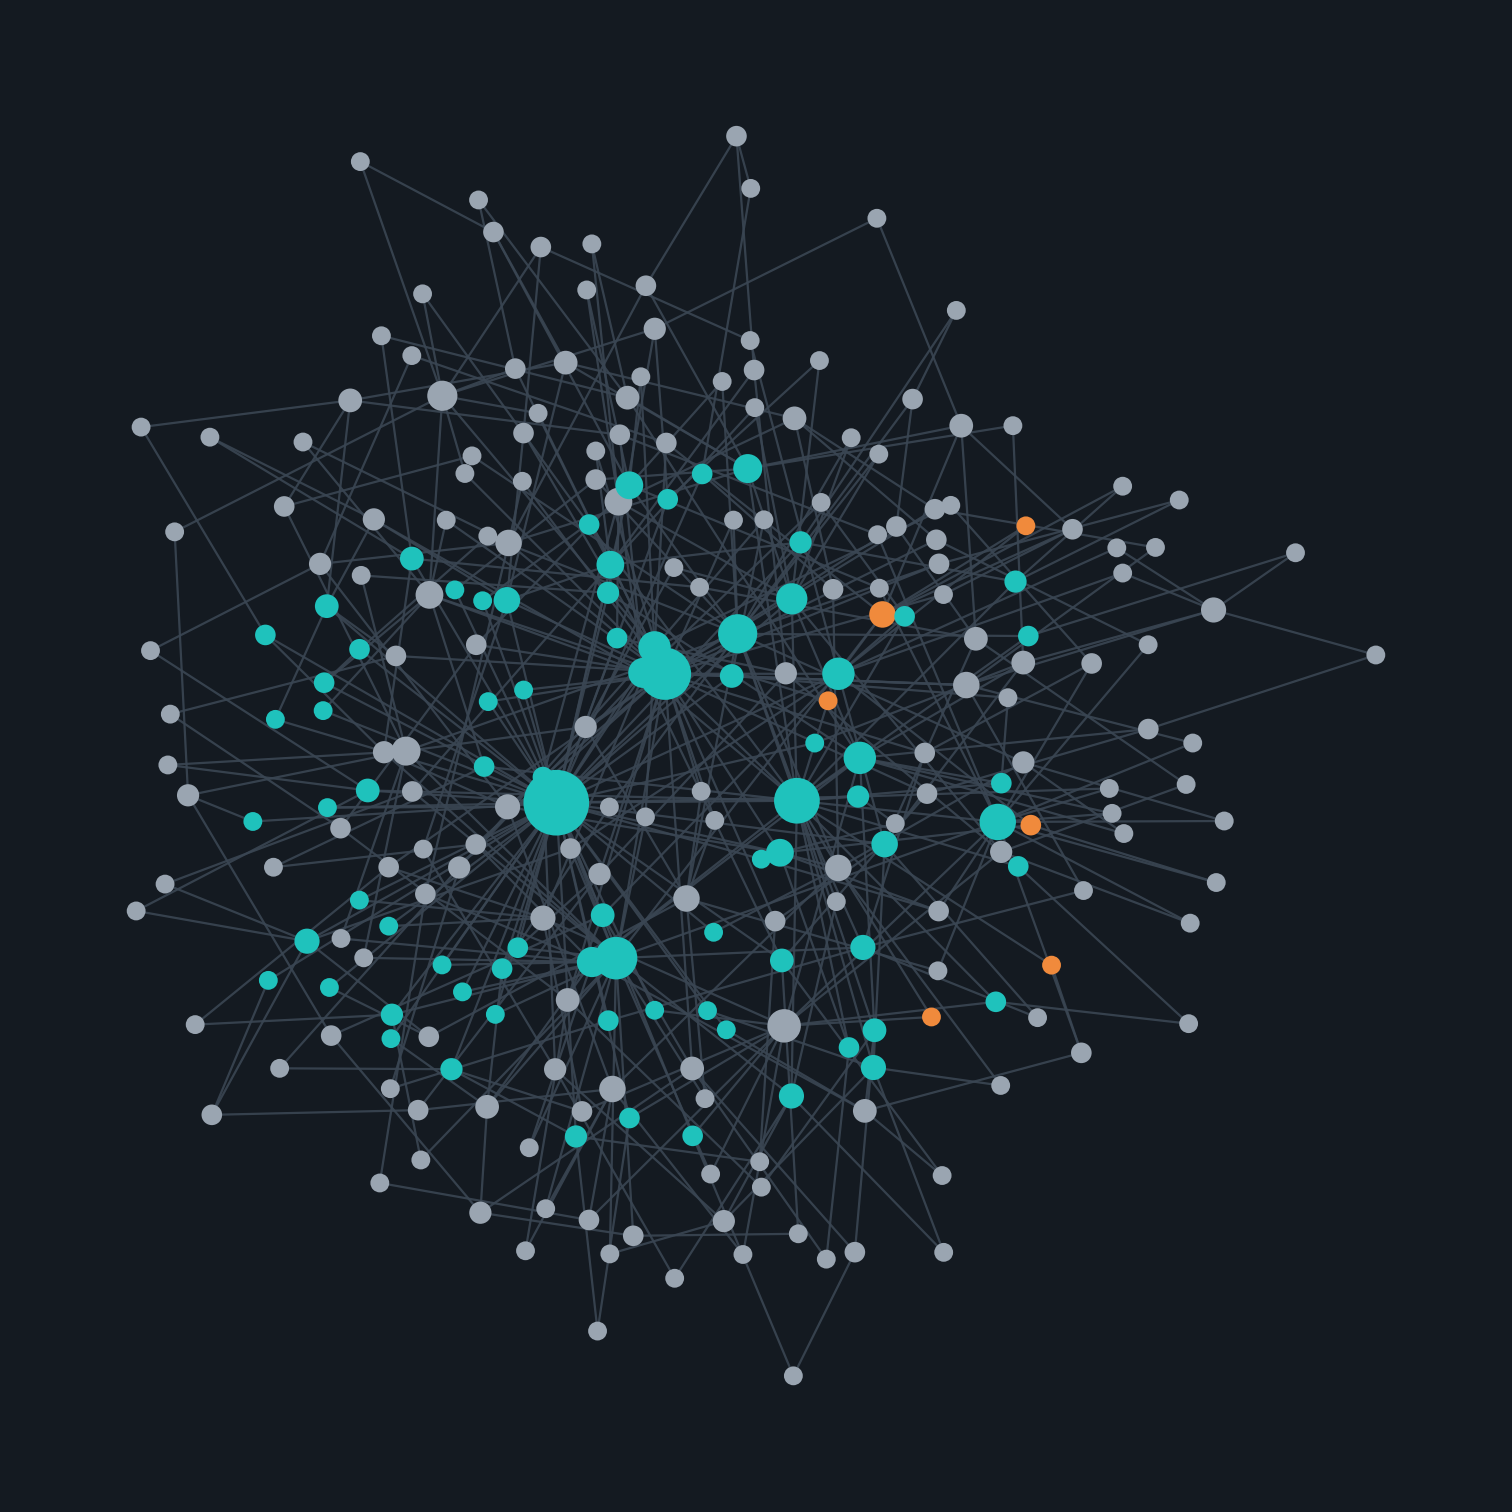
\includegraphics[width=\linewidth]{portada_red.png}
    \end{column}
  \end{columns}
\end{frame}
}
\note{\textbf{Jesus (0:40).} Buenos días. Somos Jesus, David y Duvan. Nuestro proyecto simula cómo se difunde un producto nuevo cuando cada persona decide influida por la publicidad y por sus contactos. Lo aplicamos a dos casos de actualidad: la PS5, una tecnología, y GTA\,6, un videojuego que sale este jueves. Lo construimos en NetLogo, lo calibramos con datos reales y lo usamos para comparar escenarios que no se pueden observar.}

% =================================================================== 2. motivación
\renewcommand{\seccion}{Motivación}
\begin{frame}{Dos lanzamientos, dos maneras de difundirse}
  \vskip4mm
  \begin{columns}[t,totalwidth=\textwidth]
    \begin{column}{0.31\textwidth}\cifra{\cifraPsUnidadesFin\,M}{PS5 vendidas de noviembre de 2020 a septiembre de 2026}\end{column}
    \begin{column}{0.31\textwidth}\cifra{19 nov.}{sale GTA\,6, solo para consolas de esta generación}\end{column}
    \begin{column}{0.31\textwidth}\cifra{90\,M}{vistas del primer tráiler de GTA\,6 en 24 horas}\end{column}
  \end{columns}
  \vskip8mm
  \begin{itemize}
    \item Bass: un producto se difunde por \textcolor{terracota}{publicidad} (externa) e \textcolor{azul}{imitación} (voz a voz).
    \item La PS5 crece por imitación; un gran estreno vende casi todo al salir.
  \end{itemize}
  \fuente{Sony Interactive Entertainment, Business Data \& Sales; Guinness World Records (2023).}
\end{frame}
\note{\textbf{Jesus (0:45).} La PS5 ya pasa de \cifraPsUnidadesFin\ millones de unidades, y sobre esa base sale GTA\,6 el 19 de noviembre, después de una campaña que rompió récords: 90 millones de vistas del primer tráiler en un día. Bass explicó la difusión con dos fuerzas: la publicidad, que llega a todos, y la imitación, que depende de cuántos ya adoptaron. Cuando manda la imitación sale la curva en S, como en la PS5; cuando manda la publicidad, las ventas se concentran en el lanzamiento.}

% =================================================================== 3. problema
\renewcommand{\seccion}{Problema}
\begin{frame}{El modelo agregado no ve la red social}
  \vskip2mm
  \begin{columns}[c,totalwidth=\textwidth]
    \begin{column}{0.52\textwidth}
      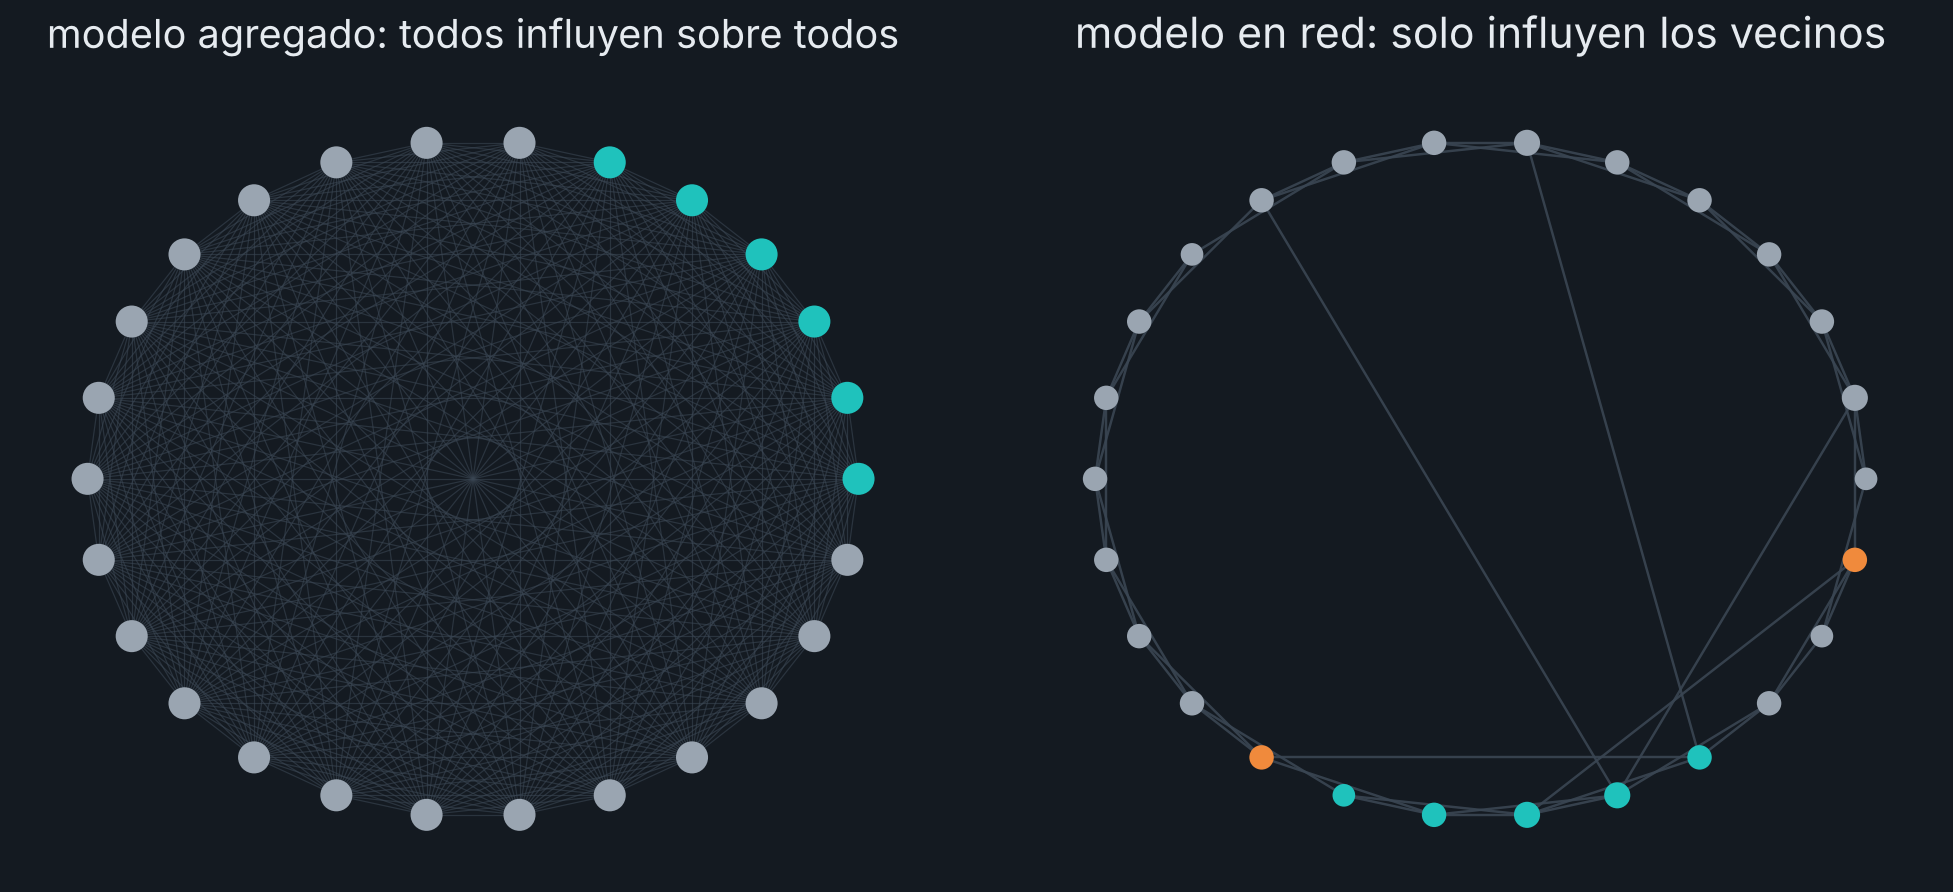
\includegraphics[width=\linewidth]{mezcla_vs_red.png}
    \end{column}
    \begin{column}{0.44\textwidth}
      \raggedright
      Bass: todos influyen sobre todos. En la realidad, solo los contactos.\par\vskip3mm
      \begin{itemize}
        \item ¿Qué pasa sin publicidad?
        \item ¿Importa la densidad o la forma de la red?
        \item ¿Cuánto se pierde con una campaña corta?
        \item ¿Responden igual una consola y un videojuego?
      \end{itemize}
    \end{column}
  \end{columns}
\end{frame}
\note{\textbf{Jesus (0:50).} El modelo de Bass describe bien las curvas agregadas, pero supone que todos influyen sobre todos, como en la red de la izquierda. En la vida real la influencia viaja por una red concreta, como la de la derecha. Eso deja cuatro preguntas sin responder: qué pasa sin publicidad, si importa la estructura de la red, cuánto se pierde con una campaña corta y si una consola y un videojuego responden igual.}

% =================================================================== 4. justificación
\renewcommand{\seccion}{Justificación}
\begin{frame}{Simular permite probar lo que no se puede observar}
  \vskip5mm
  \begin{columns}[t,totalwidth=\textwidth]
    \begin{column}{0.3\textwidth}
      {\plexmedia\color{azul}Individuos y red}\par\vskip2mm
      \nota{Cada persona es un agente con sus contactos y una regla de decisión.}
    \end{column}
    \begin{column}{0.3\textwidth}
      {\plexmedia\color{azul}Contrafactuales}\par\vskip2mm
      \nota{Lanzar sin publicidad, cambiar la red o acortar la campaña: imposible de observar en la realidad.}
    \end{column}
    \begin{column}{0.3\textwidth}
      {\plexmedia\color{azul}Datos reales}\par\vskip2mm
      \nota{PS5: calibrada y evaluada con ventas oficiales. GTA\,6, sin ventas aún: por analogía con GTA\,V.}
    \end{column}
  \end{columns}
  \vskip10mm
  \nota{NetLogo: libre, el modelo completo en un archivo y BehaviorSpace para repetir cada escenario 30 veces.}
\end{frame}
\note{\textbf{Jesus (0:50).} La simulación basada en agentes responde esas preguntas porque representa a cada persona y sus contactos, y permite correr escenarios que no se pueden observar, como lanzar sin publicidad. Para que no fuera un ejercicio solo cualitativo, la PS5 se calibró con las ventas oficiales de Sony y se evaluó con datos que no usamos para ajustar. GTA\,6 todavía no tiene ventas, así que sus parámetros salen por analogía con GTA\,V, que es la práctica estándar antes de un lanzamiento.}

% =================================================================== 5. objetivos
\renewcommand{\seccion}{Objetivos}
\begin{frame}{Qué nos propusimos}
  \vskip2mm
  {\plexmedia General.} Medir el efecto de la publicidad y de la red sobre la adopción final, en la PS5 y en GTA\,6.\par\vskip5mm
  {\plexmedia Específicos}\par\vskip1mm
  \begin{enumerate}
    \item Implementar en NetLogo el modelo de Bass en red, con tres tipos de red.
    \item Calibrar con la PS5 (entrenamiento, validación, prueba) y parametrizar GTA\,6 por analogía.
    \item Evaluar con 30 réplicas publicidad, densidad, topología y duración.
    \item Verificar con una reimplementación en Python.
  \end{enumerate}
\end{frame}
\note{\textbf{Jesus (0:40).} El objetivo general es medir el efecto de la publicidad y de la red sobre la adopción final, en la PS5 y en GTA\,6. Los específicos: implementarlo en NetLogo con tres tipos de red, calibrarlo con partición entrenamiento-validación-prueba, evaluar los escenarios con réplicas y verificarlo con una reimplementación independiente en Python.}

% =================================================================== 6. modelo
\renewcommand{\seccion}{Metodología}
\begin{frame}{Cada mes, cada persona decide: publicidad y vecinos}
  \vskip4mm
  \begin{center}{\Large $P_i = 1 - (1 - \textcolor{terracota}{p\,a_t})\,(1 - \textcolor{azul}{q\,f_i})$}\end{center}
  \vskip5mm
  \begin{columns}[T,totalwidth=\textwidth]
    \begin{column}{0.46\textwidth}
      {\color{terracota}\plexmedia publicidad}\par\nota{$p$: probabilidad mensual de que la campaña convenza; $a_t=1$ mientras está activa.}\par\vskip3mm
      {\color{azul}\plexmedia imitación}\par\nota{$q$ por $f_i$, la fracción de vecinos que ya adoptó.}
    \end{column}
    \begin{column}{0.48\textwidth}
      \vskip-\topsep
      {\small\begin{itemize}
        \item Adoptar es irreversible; todos deciden a la vez.
        \item Red completa = Bass: la diferencia es el efecto de la red.
        \item Redes aleatoria, mundo pequeño y libre de escala.
      \end{itemize}}
    \end{column}
  \end{columns}
\end{frame}
\note{\textbf{Jesus (1:00).} Cada agente es un nodo. Cada mes, quien no ha adoptado lo hace con esta probabilidad: la publicidad lo convence con probabilidad $p$ mientras la campaña esté activa, y sus vecinos con $q$ por la fracción de vecinos que ya adoptaron. Las decisiones se aplican todas a la vez al cerrar el mes y la adopción es irreversible. Si la red fuera completa, el modelo recuperaría la curva de Bass; la diferencia entre ambas es el efecto de la red. Usamos tres redes: aleatoria, mundo pequeño, con grupos cerrados, y libre de escala, con pocos nodos muy conectados. \emph{Le paso la palabra a David.}}

% =================================================================== 7. esquema
\begin{frame}{Del dato al escenario}
  \vskip2mm
  \begin{center}
  \begin{tikzpicture}[
    font=\small, text=tinta,
    caja/.style={draw=borde, line width=0.5pt, rounded corners=2pt, fill=white, align=center, inner sep=2pt,
                 minimum height=12mm, text width=21mm},
    etapa/.style={caja, fill=claro},
    flecha/.style={-{Latex[length=2mm]}, line width=0.8pt, draw=tinta},
    detalle/.style={font=\scriptsize, text=secundario}]
    \node[etapa] (d) at (0,0) {\plexmedia Datos\\[-1pt]{\scriptsize\color{secundario}Sony, Take-Two}};
    \node[etapa] (c) at (2.78,0) {\plexmedia Calibración\\[-1pt]{\scriptsize\color{secundario}Bass, analogía}};
    \node[etapa, fill=azulfondo, draw=azul, line width=0.8pt] (m) at (5.56,0) {\plexmedia Modelo\\[-1pt]{\scriptsize\color{secundario}NetLogo + nw}};
    \node[etapa] (e) at (8.34,0) {\plexmedia Escenarios\\[-1pt]{\scriptsize\color{secundario}BehaviorSpace}};
    \node[etapa] (a) at (11.12,0) {\plexmedia Análisis\\[-1pt]{\scriptsize\color{secundario}Python}};
    \draw[flecha] (d) -- (c); \draw[flecha] (c) -- (m);
    \draw[flecha] (m) -- (e); \draw[flecha] (e) -- (a);
    % interior del modelo
    \node[caja, fill=terracotafondo, draw=terracota, text width=27mm, minimum height=9mm] (camp) at (1.6,-2.5)
      {\plexmedia Campaña\\[-1pt]{\scriptsize $p\,a_t$}};
    \node[caja, fill=azulfondo, draw=azul, text width=27mm, minimum height=9mm] (red) at (1.6,-3.75)
      {\plexmedia Red social\\[-1pt]{\scriptsize $q\,f_i$}};
    \node[caja, fill=white, draw=azul, line width=0.8pt, text width=44mm, minimum height=21mm] (regla) at (6.3,-3.125)
      {\plexmedia Regla de adopción\\[4pt]$P_i = 1-(1-p\,a_t)(1-q\,f_i)$};
    \node[caja, text width=22mm, minimum height=12mm] (est) at (10.62,-3.125) {\plexmedia Estado\\[-1pt]{\scriptsize adopta y no vuelve atrás}};
    \draw[flecha, draw=terracota] (camp.east) -- (regla.west |- camp.east);
    \draw[flecha, draw=azul] (red.east) -- (regla.west |- red.east);
    \draw[flecha] (regla) -- (est);
    \begin{scope}[on background layer]
      \node[draw=azul, dashed, rounded corners=3pt, fit=(camp)(red)(regla)(est), inner sep=2.5mm] (int) {};
    \end{scope}
    \node[font=\scriptsize, text=azul, anchor=south west] at (int.north west) {cada mes, dentro del modelo};
    \draw[flecha, draw=azul, dashed] (m.south) -- (m.south |- int.north);
  \end{tikzpicture}
  \end{center}
\end{frame}
\note{\textbf{David (0:40).} Arriba el flujo: las ventas reales dan los parámetros, la PS5 por calibración de Bass y GTA\,6 por analogía con GTA\,V; NetLogo simula; BehaviorSpace corre los cuatro experimentos; Python calcula las medidas. Abajo, lo que pasa dentro del modelo cada mes: la campaña y la red alimentan la regla, que decide si cada persona adopta.}

% =================================================================== 8. implementación
\begin{frame}[fragile]{Implementación en NetLogo}
  \vskip1mm
  \begin{columns}[c,totalwidth=\textwidth]
    \begin{column}{0.47\textwidth}
      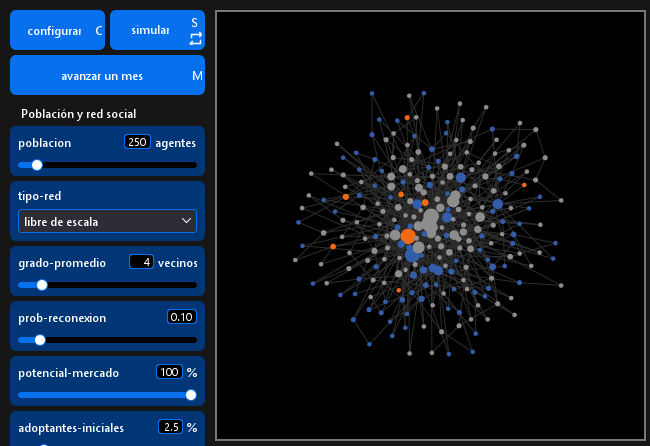
\includegraphics[width=\linewidth]{netlogo_ps5.png}\par\vskip1mm
      {\fontsize{6}{7}\selectfont\color{tenue}Interfaz del modelo (configuración de demostración: caso PS5, red libre de escala, mes 30).}
    \end{column}
    \begin{column}{0.5\textwidth}
\begin{lstlisting}
to decidir
  let p p-efectivo
  ask turtles with
      [susceptible? and not adoptante?] [
    let vecinos link-neighbors
    let f 0
    if any? vecinos [
      set f count vecinos with [adoptante?]
        / count vecinos ]
    let prob 1 - (1 - p) * (1 - q-imitacion * f)
    set decide-adoptar? random-float 1 < prob ]
end
\end{lstlisting}
      \vskip4mm
      \nota{\texttt{actualizar} aplica todas las decisiones a la vez. La extensión nw genera las redes; el selector de caso carga PS5, GTA\,6 o libre.}
    \end{column}
  \end{columns}
\end{frame}
\note{\textbf{David (0:50).} Esto es NetLogo con la extensión nw. A la izquierda, la interfaz con el caso PS5 en una red libre de escala: en azul los que ya adoptaron, en naranja los de este mes, y los nodos grandes son los más conectados. A la derecha, el procedimiento decidir: cada no adoptante cuenta qué fracción de sus vecinos ya adoptó y sortea su decisión con la fórmula. Un procedimiento aparte, actualizar, aplica todas las decisiones a la vez para que el orden de los agentes no afecte el resultado. El selector de caso carga los parámetros de la PS5 o de GTA\,6 con un clic.}

% =================================================================== 9. datos PS5
\renewcommand{\seccion}{Conjunto de datos}
\begin{frame}{La PS5: \cifraTrimestres\ trimestres de ventas oficiales de Sony}
  \begin{columns}[c,totalwidth=\textwidth]
    \begin{column}{0.6\textwidth}
      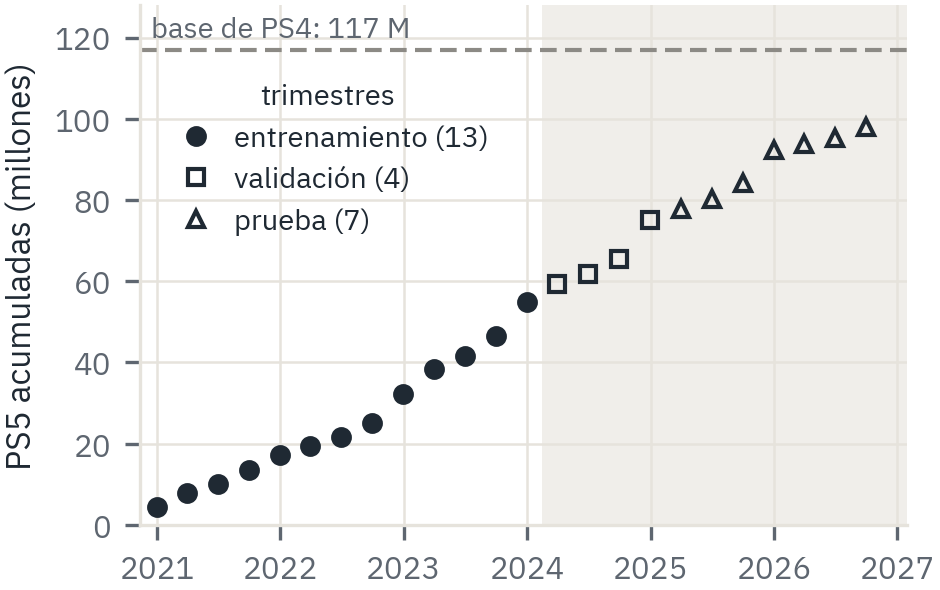
\includegraphics[width=\linewidth]{serie_ps5.png}
    \end{column}
    \begin{column}{0.36\textwidth}
      {\small\begin{itemize}
        \item \cifraPsUnidadesIni\ a \cifraPsUnidadesFin\ millones acumulados, dic.\,2020 a sep.\,2026.
        \item Adopción = acumulado / base de PS4 (\cifraUniverso\,M), fijada antes de ver la prueba.
        \item Simulación: \cifraCorridas\ corridas de 1000 agentes.
      \end{itemize}}
    \end{column}
  \end{columns}
  \fuente{Sony Interactive Entertainment, Business Data \& Sales (unidades vendidas a tiendas).}
\end{frame}
\note{\textbf{David (0:40).} La serie real son las unidades de PS5 que Sony publica cada trimestre: \cifraTrimestres\ trimestres, de \cifraPsUnidadesIni\ a \cifraPsUnidadesFin\ millones. La expresamos como porcentaje de la base de la PS4, \cifraUniverso\ millones, que fijamos antes de mirar los datos de prueba. El segundo conjunto lo genera la simulación: \cifraCorridas\ corridas de mil agentes.}

% =================================================================== 10. analogía GTA V
\begin{frame}{GTA\,6 aún no tiene ventas: lo parametrizamos con GTA\,V}
  \begin{columns}[c,totalwidth=\textwidth]
    \begin{column}{0.54\textwidth}
      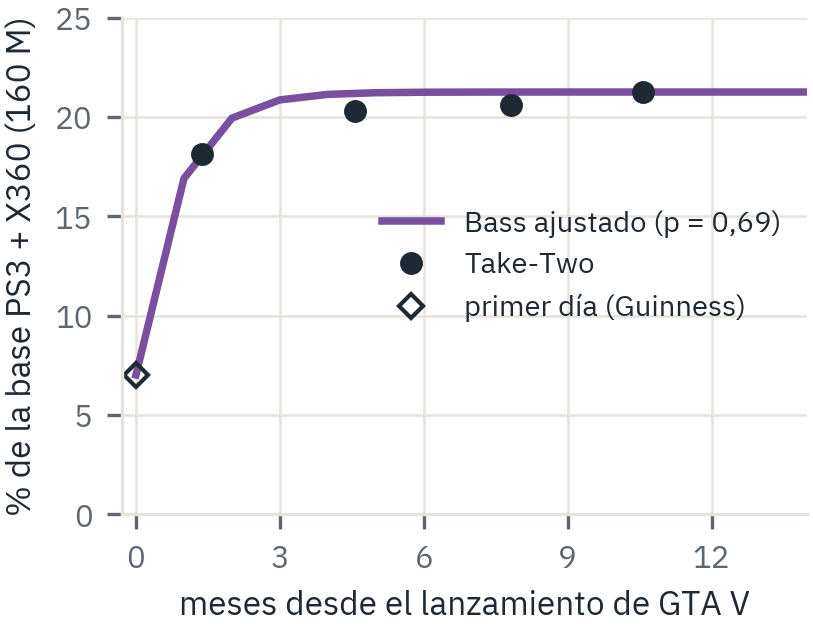
\includegraphics[width=0.94\linewidth]{analogia_gtav.png}
    \end{column}
    \begin{column}{0.42\textwidth}
      {\small\begin{itemize}
        \item GTA\,V: \cifraGtavSeisSemanas\,M en seis semanas y \cifraGtavMeseta\,M al año, sobre \cifraGtaBase\,M de consolas.
        \item Mismo ajuste de Bass: publicidad de \textcolor{terracota}{\cifraGtaP} al mes, unas \cifraGtaRazonPQ\ veces la imitación.
        \item GTA\,6 entre dueños de PS5: potencial \cifraGtaM\,\%, \cifraGtaIniciales\,\% el primer día, \cifraGtaHorizonte\ meses.
      \end{itemize}}
    \end{column}
  \end{columns}
  \fuente{Take-Two Interactive, resultados trimestrales 2013--2014; primer día: Guinness World Records (2013).}
\end{frame}
\note{\textbf{David (0:50).} GTA\,6 no tiene ventas todavía, así que usamos el método de analogía: tomamos el lanzamiento más parecido, GTA\,V. Vendió \cifraGtavSeisSemanas\ millones en seis semanas y se estabilizó en \cifraGtavMeseta\ millones, sobre \cifraGtaBase\ millones de consolas. Con la imitación fijada en la de la PS5, el ajuste atribuye el salto del lanzamiento a la publicidad: \cifraGtaP\ al mes, unas \cifraGtaRazonPQ\ veces la imitación, lo contrario de la PS5. Así modelamos GTA\,6 entre los dueños de PS5, con un potencial del \cifraGtaM\,\% y dos años de horizonte.}

% =================================================================== 11. diseño experimental
\renewcommand{\seccion}{Diseño experimental}
\begin{frame}{Cuatro experimentos, 30 réplicas por escenario}
  \vskip2mm
  \begin{tikzpicture}[x=1mm, y=1mm, font=\scriptsize]
    \fill[azul] (0,0) rectangle (60,10);
    \fill[azulclaro] (61,0) rectangle (92,10);
    \fill[terracota] (93,0) rectangle (134,10);
    \node[text=white, align=center] at (30,5) {entrenamiento\\dic.\,2020--dic.\,2023 · \cifraObsEnt\ trimestres};
    \node[text=tinta, align=center] at (76.5,5) {validación\\2024 · \cifraObsVal\ trimestres};
    \node[text=white, align=center] at (113.5,5) {prueba\\2025--2026 · \cifraObsPru\ trimestres};
    \node[text=secundario] at (30,-3) {ajusta $p$ y $q$};
    \node[text=secundario] at (76.5,-3) {elige $m$ y la red};
    \node[text=secundario] at (113.5,-3) {solo evalúa};
  \end{tikzpicture}
  \vskip6mm
  {\footnotesize
  \begin{tabular}{@{}lp{0.74\textwidth}r@{}}
    \toprule
    & factores (E1 a E3 para ambos casos: PS5 y GTA\,6) & corridas\\
    \midrule
    E1 & publicidad \{sin, con\} $\times$ densidad $k$ = 2, 4, 6, 8, 12, 16 & 720\\
    E2 & publicidad $\times$ topología \{aleatoria, mundo pequeño, libre de escala\} & 360\\
    E3 & duración de la campaña \{0, 1, 3, 6, 12, 24 meses, permanente\} & 420\\
    E4 & calibración PS5: 3 topologías $\times$ $k$ = 4, 8, 16 & 270\\
    \bottomrule
  \end{tabular}}
\end{frame}
\note{\textbf{David (0:50).} La serie de la PS5 se parte en el tiempo: con entrenamiento estimamos $p$ y $q$; como el potencial no se puede estimar en plena fase de crecimiento, lo elegimos en validación, igual que la red; la prueba solo evalúa. Corremos cuatro experimentos, los tres de escenarios para los dos casos: publicidad por densidad, publicidad por topología y duración de la campaña, más la calibración. Cada combinación se repite 30 veces. \emph{Duvan presenta las medidas y los resultados.}}

% =================================================================== 12. medidas
\renewcommand{\seccion}{Medidas de desempeño}
\begin{frame}{Cómo medimos}
  \vskip4mm
  \begin{columns}[T,totalwidth=\textwidth]
    \begin{column}{0.47\textwidth}
      {\plexmedia\color{azul}Escenarios}\par\vskip1mm
      {\small\begin{itemize}
        \item \alert{Adopción final}: \% de la población que adoptó al final del período (PS5: \cifraHorizontePs\ meses; GTA\,6: \cifraHorizonteGta).
        \item Mes del 50\,\% y mes del pico de compras.
        \item Media e IC del 95\,\% con 30 réplicas.
      \end{itemize}}
    \end{column}
    \begin{column}{0.47\textwidth}
      {\plexmedia\color{azul}Ajuste a la serie real}\par\vskip1mm
      {\small\begin{itemize}
        \item RMSE: raíz del error cuadrático medio, en puntos porcentuales.
        \item MAPE: error porcentual absoluto medio.
        \item Por partición: entrenamiento, validación y prueba.
      \end{itemize}}
    \end{column}
  \end{columns}
\end{frame}
\note{\textbf{Duvan (0:30).} La medida principal, la que pide el enunciado, es el porcentaje de adopción al final del período: seis años para la PS5 y dos para GTA\,6. La complementamos con el mes del 50\,\% y el mes del pico de compras. Frente a la serie real usamos RMSE y MAPE por partición. Todo con 30 réplicas e intervalos del 95\,\%.}

% =================================================================== 13. calibración
\renewcommand{\seccion}{Resultados}
\begin{frame}{El modelo sigue la serie de prueba de la PS5}
  \begin{columns}[c,totalwidth=\textwidth]
    \begin{column}{0.64\textwidth}
      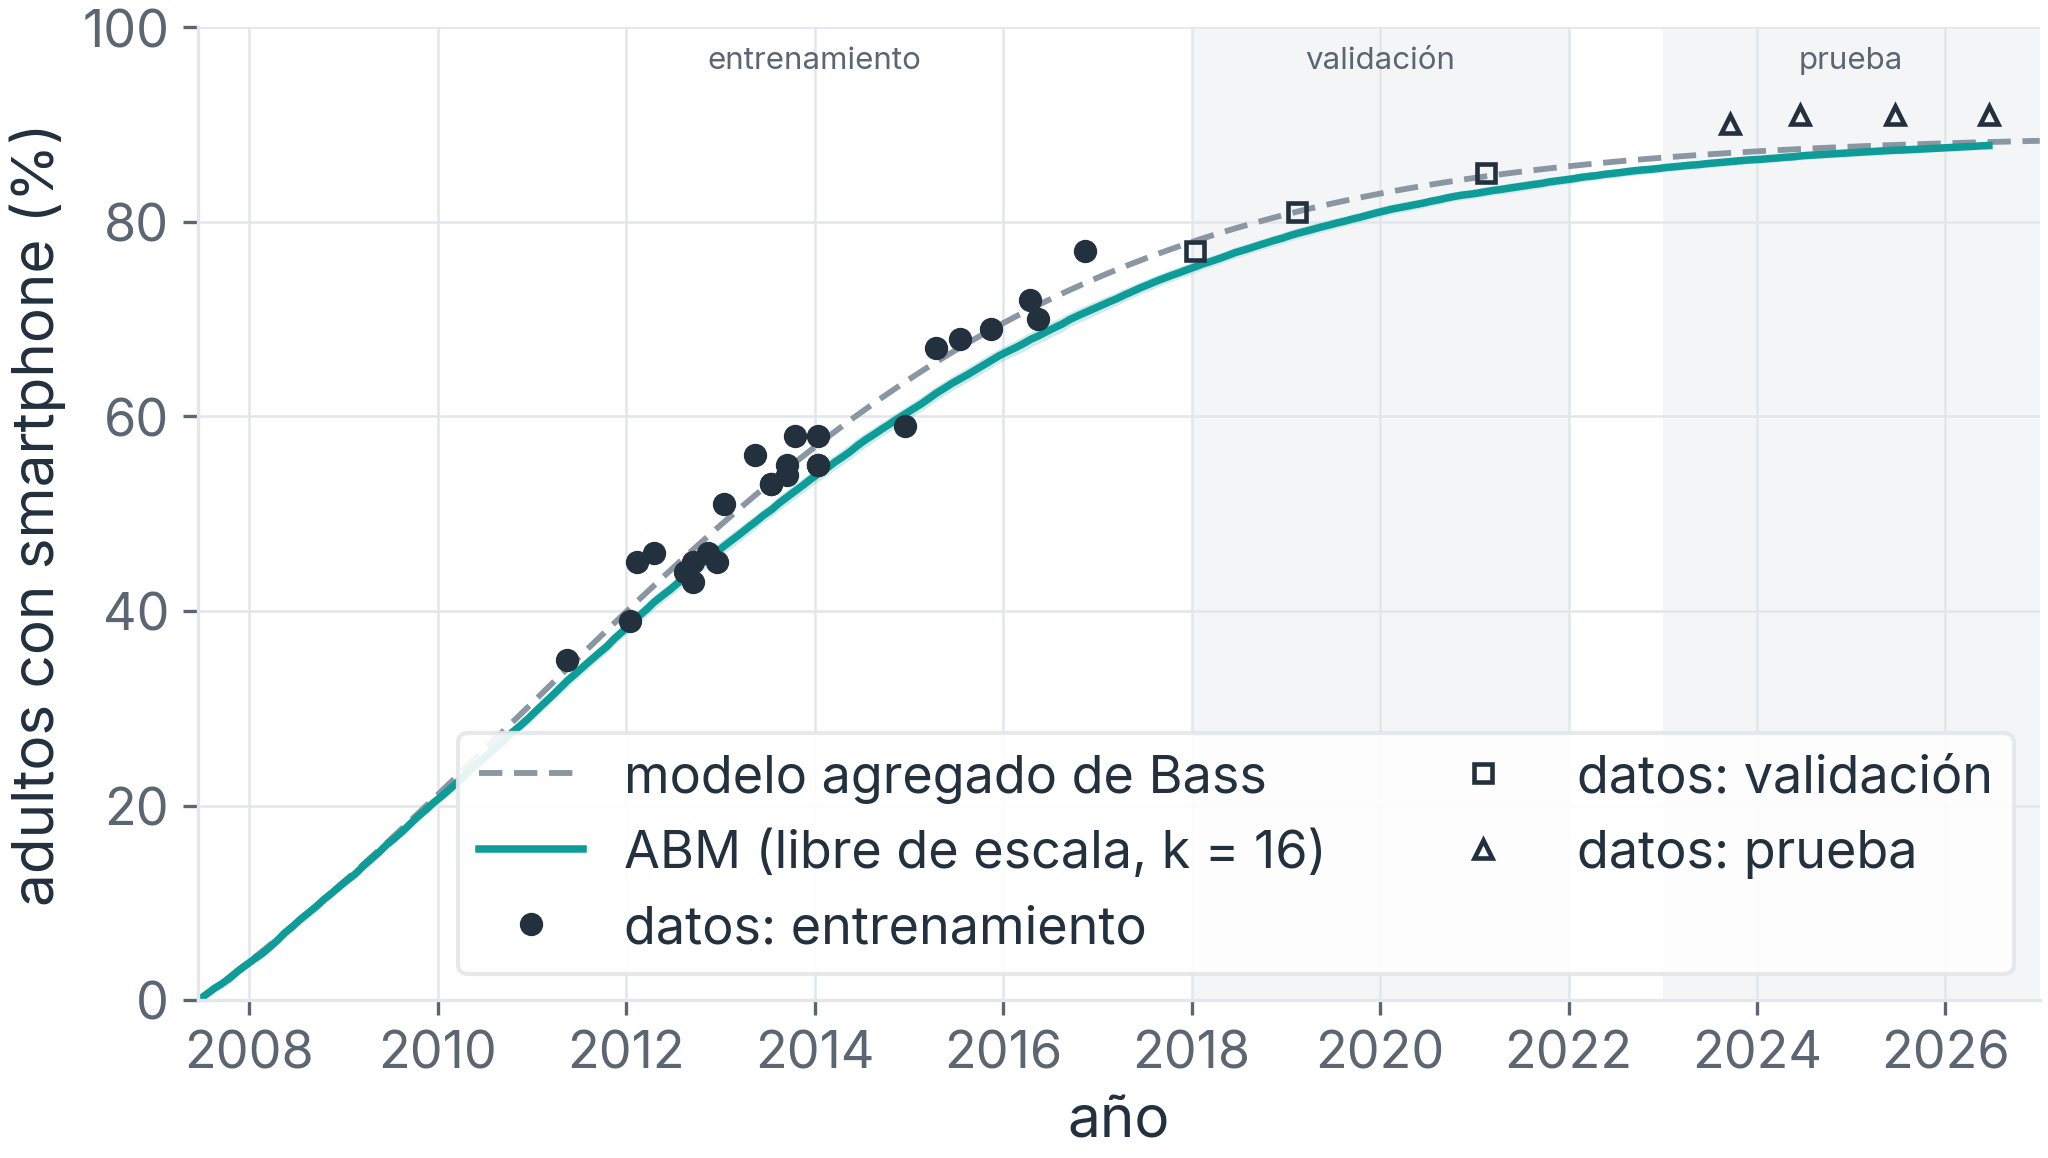
\includegraphics[width=\linewidth]{fig_calibracion.png}
    \end{column}
    \begin{column}{0.32\textwidth}
      \cifra{\cifraAbmRmsePru\ pp}{error en prueba del modelo de agentes (Bass: \cifraBassRmsePru)}\par\vskip5mm
      \nota{Bass anual: $p$\,=\,\cifraBassP, $q$\,=\,\cifraBassQ; la imitación pesa \cifraBassRazonQP\ veces más. Red elegida en validación: \cifraAbmSelRedNombre, $k$\,=\,\cifraAbmSelK.}
    \end{column}
  \end{columns}
\end{frame}
\note{\textbf{Duvan (0:50).} El ajuste da $p$ = \cifraBassP\ y $q$ = \cifraBassQ\ anuales: en la PS5 la imitación pesa \cifraBassRazonQP\ veces más que la publicidad. En validación se eligió la \cifraAbmSelRedNombre\ con $k$ = \cifraAbmSelK. En prueba, que nunca usamos para ajustar, el error es de \cifraAbmRmsePru\ puntos, mayor que el de Bass, \cifraBassRmsePru, porque la red frena la difusión. Ambos quedan un poco por debajo del dato de Sony de noviembre de 2026, más de 100 millones: la PS5 probablemente superará la base de la PS4.}

% =================================================================== 14. publicidad
\begin{frame}{Sin publicidad, ninguno de los dos llega lejos}
  \vskip1mm
  \begin{center}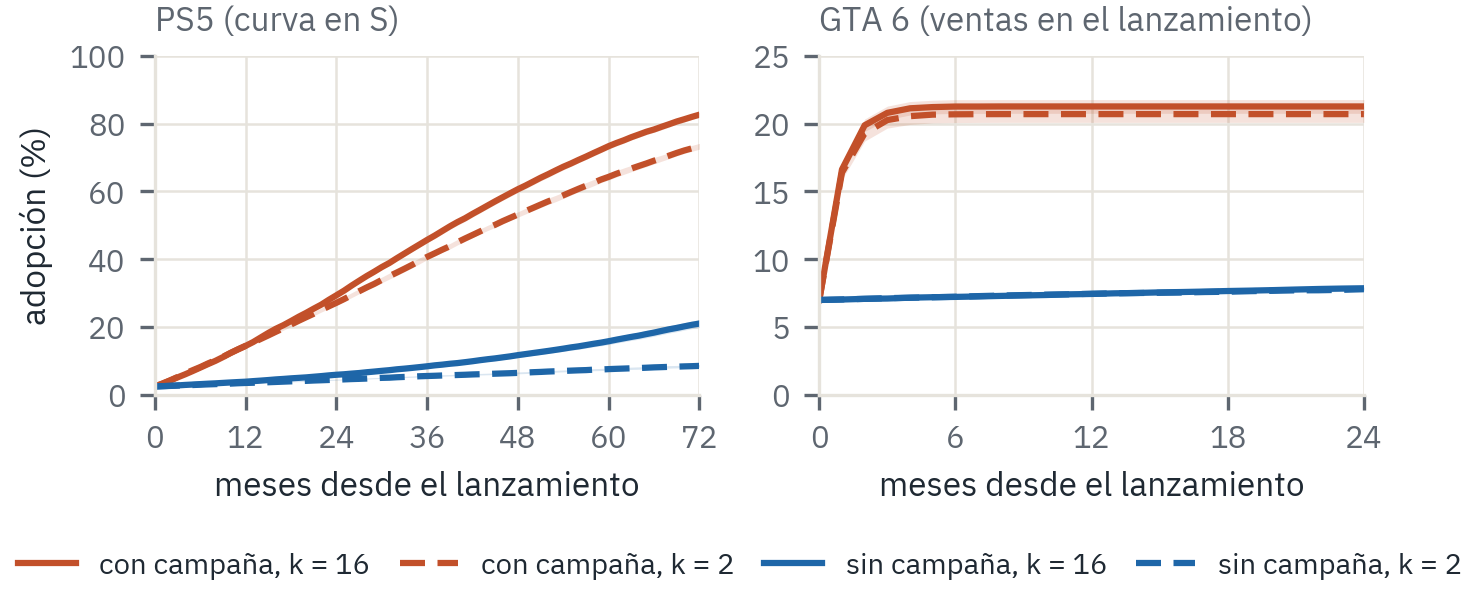
\includegraphics[width=0.9\linewidth]{publicidad_casos.png}\end{center}
  \vskip-3mm
  \nota{Red de mundo pequeño con $k$\,=\,2 (discontinua) y 16 (continua).}
\end{frame}
\note{\textbf{Duvan (0:50).} El resultado central. En la PS5, sin publicidad la adopción queda entre el \cifraPsSinMin\ y el \cifraPsSinMax\,\% en seis años; con campaña, entre el \cifraPsConMin\ y el \cifraPsConMax\,\%, con la curva en S. En GTA\,6 la campaña lo decide todo: con ella se alcanza el potencial casi en el primer mes; sin ella la adopción apenas pasa de los compradores del primer día. Sin publicidad, la PS5 simplemente no despega.}

% =================================================================== 15. densidad y topología
\begin{frame}{La red pesa sobre todo cuando no hay publicidad}
  \begin{columns}[c,totalwidth=\textwidth]
    \begin{column}{0.66\textwidth}
      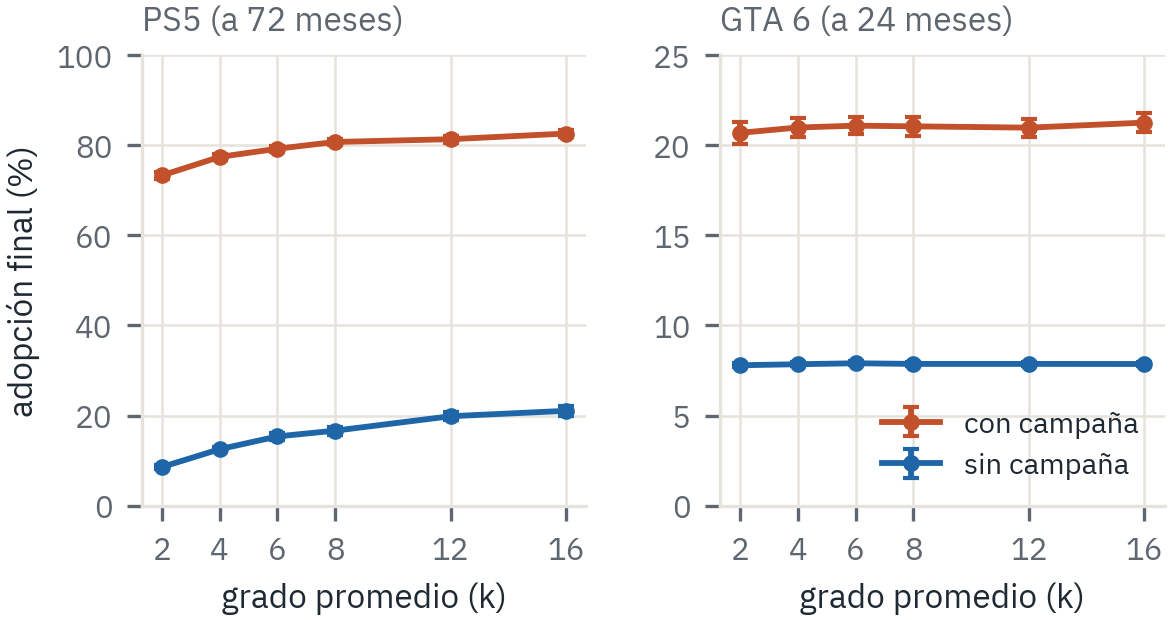
\includegraphics[width=\linewidth]{densidad.png}
    \end{column}
    \begin{column}{0.3\textwidth}
      \cifra{×\,\cifraPsSinRazon}{adopción de la PS5 sin campaña al pasar de $k$\,=\,2 a 16}\par\vskip4mm
      \nota{Con campaña, la misma diferencia solo la multiplica por \cifraPsConRazon. Sin campaña, la red de mundo pequeño es la topología más lenta.}
    \end{column}
  \end{columns}
\end{frame}
\note{\textbf{Duvan (0:50).} En la PS5 sin publicidad, pasar de 2 a 16 contactos multiplica la adopción por \cifraPsSinRazon; con campaña solo por \cifraPsConRazon, porque la publicidad siembra adoptantes en toda la red. En la topología pasa lo mismo: sin campaña, la red de mundo pequeño es la más lenta de las tres, porque sus grupos cerrados atrapan la influencia, y la libre de escala la más variable, porque depende de si un nodo muy conectado adopta temprano. En GTA\,6 la red casi no cambia nada.}

% =================================================================== 16. duración
\begin{frame}{GTA\,6: basta un mes; PS5: la campaña necesita tiempo}
  \begin{columns}[c,totalwidth=\textwidth]
    \begin{column}{0.58\textwidth}
      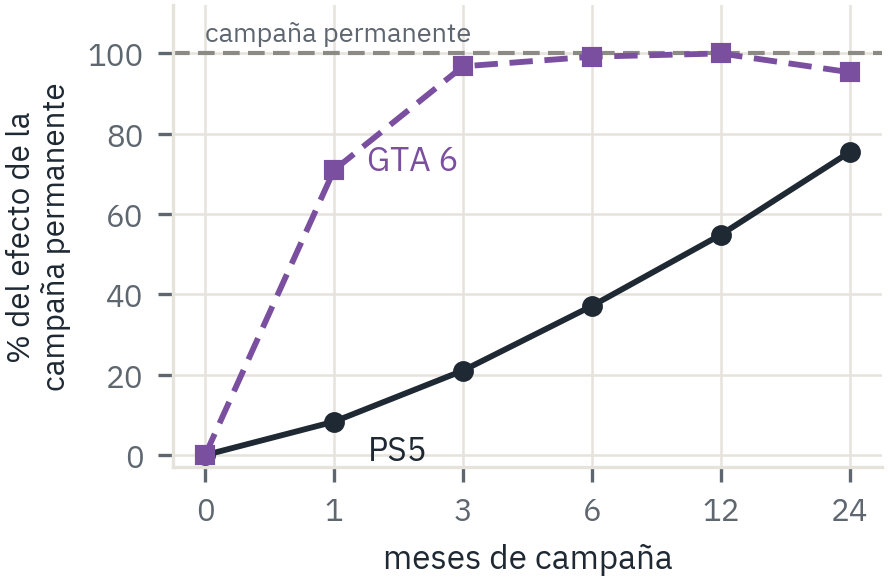
\includegraphics[width=\linewidth]{fraccion_duracion.png}
    \end{column}
    \begin{column}{0.38\textwidth}
      \cifra{\cifraFraccionGtaDUno\,\%}{del efecto de una campaña permanente se logra con un mes en GTA\,6}\par\vskip5mm
      \cifra{\cifraFraccionPsDDoce\,\%}{se logra con un año en la PS5 (dos años: \cifraFraccionPsDVeinticuatro\,\%)}
    \end{column}
  \end{columns}
\end{frame}
\note{\textbf{Duvan (0:40).} Si la campaña se corta, ¿cuánto se pierde? En GTA\,6, un solo mes ya logra el \cifraFraccionGtaDUno\,\% del efecto de una campaña permanente: el lanzamiento concentra casi todo. En la PS5 el rendimiento es gradual: un año logra el \cifraFraccionPsDDoce\,\% y dos años el \cifraFraccionPsDVeinticuatro\,\%, porque la imitación necesita tiempo para sostener la difusión. Los puntos de GTA\,6 que pasan apenas del 100\,\% son variación entre réplicas. \emph{David hace la demostración.}}

% =================================================================== 17. demo
\renewcommand{\seccion}{Demostración}
\begin{frame}{En vivo en NetLogo}
  \vskip1mm
  \begin{columns}[c,totalwidth=\textwidth]
    \begin{column}{0.4\textwidth}
      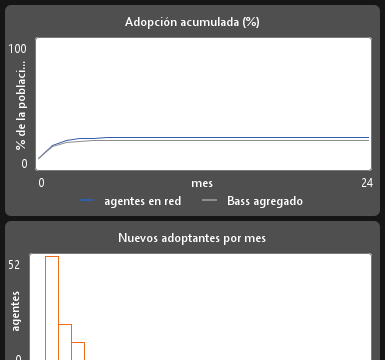
\includegraphics[width=0.86\linewidth]{netlogo_gta6.png}\par\vskip1mm
      {\fontsize{6}{7}\selectfont\color{tenue}Caso GTA\,6: compras concentradas en el primer mes.}
    \end{column}
    \begin{column}{0.56\textwidth}
      {\small\begin{enumerate}
        \item Caso \alert{GTA\,6} $\to$ configurar $\to$ simular: el pico llega en el primer mes.
        \item Campaña apagada: la adopción apenas pasa del \cifraGtaIniciales\,\%.
        \item Caso \textcolor{azul}{PS5}: curva en S frente a la de Bass.
      \end{enumerate}}
      \vskip2mm
      \nota{Si sobra tiempo: PS5 sin campaña y $k$ de 16 a 2; Herramientas $\to$ BehaviorSpace.}
    \end{column}
  \end{columns}
\end{frame}
\note{\textbf{David (1:10).} Demostración en vivo; los pasos están en el guion. Hacer 1 a 3; los otros dos solo si sobra tiempo.}

% =================================================================== 18. conclusiones
\renewcommand{\seccion}{Conclusiones}
\begin{frame}{Publicidad primero, red después}
  \vskip2mm
  \begin{enumerate}
    \item PS5: sin campaña, a lo sumo \cifraPsSinMaxGlobal\,\%; con campaña, al menos \cifraPsConMin\,\%.
    \item GTA\,6: un mes de campaña logra el \cifraFraccionGtaDUno\,\% del efecto.
    \item La red pesa sobre todo cuando no hay publicidad.
    \item Error en prueba: \cifraAbmRmsePru\ pp; la reimplementación en Python coincide.
  \end{enumerate}
  \vskip5mm
  \nota{Limitaciones: coeficientes iguales para todos, red fija, unidades vendidas a tiendas y parámetros de GTA\,6 hipotéticos.}
\end{frame}
\note{\textbf{Duvan (0:30).} Cuatro conclusiones. En la PS5, la publicidad es la condición del despegue. En GTA\,6, el primer mes de campaña decide el resultado. La red pesa sobre todo cuando no hay publicidad. Y el modelo quedó validado con datos que no usamos para ajustar y verificado con una reimplementación independiente.}

% =================================================================== 19. referencias
\renewcommand{\seccion}{Referencias}
\begin{frame}{Fuentes}
  \vskip0.5mm
  \raggedright\fontsize{8}{9.6}\selectfont
  \setlength{\parskip}{1.1mm}
  \referencia{Bass, F.\,M. (1969). A new product growth model for consumer durables. \textit{Management Science}, 15(5), 215--227.}
  \referencia{Goldenberg, J., Libai, B. y Muller, E. (2001). Talk of the network. \textit{Marketing Letters}, 12(3), 211--223.}
  \referencia{Rogers, E.\,M. (2003). \textit{Diffusion of Innovations} (5.ª ed.). Free Press.}
  \referencia{Thomas, R.\,J. (1985). Estimating market growth for new products: an analogical diffusion model approach. \textit{Journal of Product Innovation Management}, 2(1), 45--55.}
  \referencia{Watts, D.\,J. y Strogatz, S.\,H. (1998). Collective dynamics of `small-world' networks. \textit{Nature}, 393, 440--442.}
  \referencia{Wilensky, U. (1999). NetLogo. Northwestern University.}
  \referencia{Sony Interactive Entertainment (2026). Business Data \& Sales.}
  \referencia{Take-Two Interactive (2013--2014). Resultados trimestrales, años fiscales 2014 y 2015.}
  \referencia{Guinness World Records (2013, 2023). Récords de ventas de GTA\,V y de vistas del tráiler de GTA\,6.}
\end{frame}
\note{\textbf{Duvan (0:10).} Las referencias están en pantalla. Gracias; quedamos atentos a sus preguntas.}

\end{document}
"  -> notas del orador
% Las cifras salen de ../articulo/tablas/cifras.tex (analisis/analisis_resultados.py) y las
% figuras de ../analisis/figuras/diapositivas (analisis/figuras_diapositivas.py).
\ifdefined\connotas
  \documentclass[aspectratio=169,11pt,notes=only]{beamer}
\else
  \documentclass[aspectratio=169,11pt]{beamer}
\fi

\usepackage{fontspec}
\usepackage[spanish,es-noshorthands]{babel}
\usepackage{booktabs}
\usepackage{tikz}
\usepackage{listings}
\usetikzlibrary{arrows.meta,positioning,calc,fit,backgrounds}

% ------------------------------------------------------------------ tipografía
\setsansfont{IBMPlexSans}[Path=../analisis/fuentes/, Extension=.ttf, UprightFont=*-Regular,
  BoldFont=*-SemiBold, ItalicFont=*-Regular, ItalicFeatures={FakeSlant=0.18}]
\newfontfamily\plexmedia{IBMPlexSans-Medium}[Path=../analisis/fuentes/, Extension=.ttf]
\usefonttheme{professionalfonts}
\usefonttheme[onlymath]{serif}
\hyphenpenalty=10000
\exhyphenpenalty=10000

% ------------------------------------------------------------------ colores
% terracota = publicidad (con campaña), azul = imitación (sin campaña), igual que en el modelo y las figuras
\definecolor{papel}{HTML}{FBFAF6}
\definecolor{tinta}{HTML}{1F2933}
\definecolor{secundario}{HTML}{5E6670}
\definecolor{tenue}{HTML}{8C8A85}
\definecolor{borde}{HTML}{B9B4AA}
\definecolor{claro}{HTML}{F1EEE7}
\definecolor{azul}{HTML}{1E66A8}
\definecolor{azulclaro}{HTML}{8DB3D6}
\definecolor{azulfondo}{HTML}{E4EDF6}
\definecolor{terracota}{HTML}{C2502A}
\definecolor{terracotafondo}{HTML}{F7E6DE}

\setbeamercolor{background canvas}{bg=papel}
\setbeamercolor{normal text}{fg=tinta}
\setbeamercolor{structure}{fg=azul}
\setbeamercolor{frametitle}{fg=tinta}
\setbeamercolor{alerted text}{fg=terracota}
\setbeamercolor{item}{fg=terracota}
\setbeamercolor{enumerate item}{fg=terracota}

% ------------------------------------------------------------------ plantillas
\setbeamertemplate{navigation symbols}{}
\setbeamersize{text margin left=13mm, text margin right=13mm}
\setbeamerfont{frametitle}{size=\Large}
\newcommand{\seccion}{}
\setbeamertemplate{frametitle}{%
  \vskip6mm%
  {\scriptsize\addfontfeatures{LetterSpace=12}\color{terracota}\MakeUppercase{\seccion}}\par\vskip1mm%
  {\usebeamerfont{frametitle}\plexmedia\color{tinta}\insertframetitle\par}\vskip0.5mm}
\setbeamertemplate{footline}{%
  \hbox to \paperwidth{\hskip13mm{\fontsize{6}{7}\selectfont\color{tenue}Delgado · Monroy · Baquero\quad Universidad de los Llanos}%
  \hfill{\fontsize{6}{7}\selectfont\color{tenue}\insertframenumber\,/\,\inserttotalframenumber}\hskip13mm}\vskip4mm}
\setbeamertemplate{itemize item}{\raisebox{0.3ex}{\color{terracota}\rule{0.8ex}{0.8ex}}}
\setbeamertemplate{enumerate item}{\color{terracota}\plexmedia\insertenumlabel.}
\setbeamertemplate{itemize/enumerate body begin}{\raggedright}
\setlength{\leftmargini}{1.3em}
\setbeamertemplate{note page}{\vskip5mm\hskip6mm\begin{minipage}[t]{0.42\paperwidth}\vskip0pt\insertslideintonotes{0.4}\end{minipage}%
  \hskip4mm\begin{minipage}[t]{0.4\paperwidth}\vskip0pt\raggedright\footnotesize
  {\scriptsize\color{terracota}DIAPOSITIVA \insertframenumber}\par\vskip2mm\insertnote\end{minipage}}

\lstset{basicstyle=\ttfamily\fontsize{7.2}{8.6}\selectfont\color{tinta}, keywordstyle=\color{azul}, columns=fullflexible,
  keepspaces=true, frame=none, aboveskip=0pt, belowskip=0pt,
  morekeywords={to,end,ask,let,set,if,with,count,any?,random-float,turtles,link-neighbors,not}}

% ------------------------------------------------------------------ utilidades
\newcommand{\cifra}[2]{% número grande + leyenda
  \begin{minipage}[t]{\linewidth}\raggedright{\plexmedia\fontsize{24}{26}\selectfont\color{azul}#1\par}\vskip1mm
  {\small\color{secundario}#2\par}\end{minipage}}
\newcommand{\nota}[1]{{\raggedright\footnotesize\color{secundario}#1\par}}
\newcommand{\fuente}[1]{\par\vfill{\fontsize{6}{7}\selectfont\color{tenue}#1}\par\vskip1mm}
\newcommand{\referencia}[1]{\par\hangindent=1.4em\hangafter=1 #1\par}

% generado por analisis_resultados.py
\newcommand{\cifraBassP}{0,079}
\newcommand{\cifraBassQ}{0,242}
\newcommand{\cifraBassM}{89}
\newcommand{\cifraBassPmes}{0,0066}
\newcommand{\cifraBassQmes}{0,0202}
\newcommand{\cifraBassPico}{3,5}
\newcommand{\cifraBassRmseEnt}{2,29}
\newcommand{\cifraBassMapeEnt}{3,64}
\newcommand{\cifraBassRmseVal}{0,63}
\newcommand{\cifraBassMapeVal}{0,60}
\newcommand{\cifraBassRmsePru}{3,10}
\newcommand{\cifraBassMapePru}{3,40}
\newcommand{\cifraAbmSelRed}{libre de escala}
\newcommand{\cifraAbmSelK}{16}
\newcommand{\cifraAbmRmseEnt}{3,52}
\newcommand{\cifraAbmRmseVal}{1,93}
\newcommand{\cifraAbmRmsePru}{3,74}
\newcommand{\cifraAbmMapePru}{4,10}
\newcommand{\cifraAbmFinal}{87,8}
\newcommand{\cifraAbmRmseValMax}{4,90}
\newcommand{\cifraAbmRmsePruMax}{5,37}
\newcommand{\cifraAbmPeorRed}{aleatoria}
\newcommand{\cifraAbmPeorK}{4}
\newcommand{\cifraSinCalKDos}{8,1}
\newcommand{\cifraSinCalKDosIc}{0,3}
\newcommand{\cifraTcincuentaSinCalKDos}{--}
\newcommand{\cifraSinCalKCuatro}{11,2}
\newcommand{\cifraSinCalKCuatroIc}{0,5}
\newcommand{\cifraTcincuentaSinCalKCuatro}{--}
\newcommand{\cifraSinCalKSeis}{13,2}
\newcommand{\cifraSinCalKSeisIc}{0,7}
\newcommand{\cifraTcincuentaSinCalKSeis}{--}
\newcommand{\cifraSinCalKOcho}{14,9}
\newcommand{\cifraSinCalKOchoIc}{0,8}
\newcommand{\cifraTcincuentaSinCalKOcho}{--}
\newcommand{\cifraSinCalKDoce}{15,1}
\newcommand{\cifraSinCalKDoceIc}{0,8}
\newcommand{\cifraTcincuentaSinCalKDoce}{--}
\newcommand{\cifraSinCalKDieciseis}{16,9}
\newcommand{\cifraSinCalKDieciseisIc}{1,0}
\newcommand{\cifraTcincuentaSinCalKDieciseis}{--}
\newcommand{\cifraConCalKDos}{79,8}
\newcommand{\cifraConCalKDosIc}{0,6}
\newcommand{\cifraTcincuentaConCalKDos}{63}
\newcommand{\cifraConCalKCuatro}{82,9}
\newcommand{\cifraConCalKCuatroIc}{0,5}
\newcommand{\cifraTcincuentaConCalKCuatro}{62}
\newcommand{\cifraConCalKSeis}{83,8}
\newcommand{\cifraConCalKSeisIc}{0,6}
\newcommand{\cifraTcincuentaConCalKSeis}{59}
\newcommand{\cifraConCalKOcho}{84,4}
\newcommand{\cifraConCalKOchoIc}{0,6}
\newcommand{\cifraTcincuentaConCalKOcho}{59}
\newcommand{\cifraConCalKDoce}{85,5}
\newcommand{\cifraConCalKDoceIc}{0,5}
\newcommand{\cifraTcincuentaConCalKDoce}{58}
\newcommand{\cifraConCalKDieciseis}{85,4}
\newcommand{\cifraConCalKDieciseisIc}{0,6}
\newcommand{\cifraTcincuentaConCalKDieciseis}{59}
\newcommand{\cifraSinLitKDos}{11,8}
\newcommand{\cifraSinLitKDosIc}{0,5}
\newcommand{\cifraTcincuentaSinLitKDos}{--}
\newcommand{\cifraSinLitKCuatro}{18,9}
\newcommand{\cifraSinLitKCuatroIc}{0,7}
\newcommand{\cifraTcincuentaSinLitKCuatro}{--}
\newcommand{\cifraSinLitKSeis}{24,2}
\newcommand{\cifraSinLitKSeisIc}{0,8}
\newcommand{\cifraTcincuentaSinLitKSeis}{--}
\newcommand{\cifraSinLitKOcho}{27,0}
\newcommand{\cifraSinLitKOchoIc}{1,1}
\newcommand{\cifraTcincuentaSinLitKOcho}{--}
\newcommand{\cifraSinLitKDoce}{35,0}
\newcommand{\cifraSinLitKDoceIc}{1,2}
\newcommand{\cifraTcincuentaSinLitKDoce}{--}
\newcommand{\cifraSinLitKDieciseis}{35,9}
\newcommand{\cifraSinLitKDieciseisIc}{1,5}
\newcommand{\cifraTcincuentaSinLitKDieciseis}{--}
\newcommand{\cifraConLitKDos}{87,7}
\newcommand{\cifraConLitKDosIc}{0,6}
\newcommand{\cifraTcincuentaConLitKDos}{54}
\newcommand{\cifraConLitKCuatro}{91,3}
\newcommand{\cifraConLitKCuatroIc}{0,4}
\newcommand{\cifraTcincuentaConLitKCuatro}{52}
\newcommand{\cifraConLitKSeis}{93,2}
\newcommand{\cifraConLitKSeisIc}{0,4}
\newcommand{\cifraTcincuentaConLitKSeis}{48}
\newcommand{\cifraConLitKOcho}{93,8}
\newcommand{\cifraConLitKOchoIc}{0,3}
\newcommand{\cifraTcincuentaConLitKOcho}{48}
\newcommand{\cifraConLitKDoce}{94,0}
\newcommand{\cifraConLitKDoceIc}{0,3}
\newcommand{\cifraTcincuentaConLitKDoce}{48}
\newcommand{\cifraConLitKDieciseis}{94,2}
\newcommand{\cifraConLitKDieciseisIc}{0,4}
\newcommand{\cifraTcincuentaConLitKDieciseis}{48}
\newcommand{\cifraDensidadGananciaCon}{6}
\newcommand{\cifraDensidadRazonSinCal}{2,1}
\newcommand{\cifraDensidadRazonSinLit}{3,0}
\newcommand{\cifraTopoSinCalAleatoria}{15,4}
\newcommand{\cifraTopoSinCalAleatoriaIc}{0,9}
\newcommand{\cifraTopoSinCalAleatoriaDe}{2,3}
\newcommand{\cifraTopoSinCalAleatoriaProp}{0}
\newcommand{\cifraTopoSinCalEscala}{13,1}
\newcommand{\cifraTopoSinCalEscalaIc}{1,2}
\newcommand{\cifraTopoSinCalEscalaDe}{3,3}
\newcommand{\cifraTopoSinCalEscalaProp}{0}
\newcommand{\cifraTopoSinCalMundo}{12,9}
\newcommand{\cifraTopoSinCalMundoIc}{0,5}
\newcommand{\cifraTopoSinCalMundoDe}{1,4}
\newcommand{\cifraTopoSinCalMundoProp}{0}
\newcommand{\cifraTopoConCalAleatoria}{83,6}
\newcommand{\cifraTopoConCalAleatoriaIc}{0,6}
\newcommand{\cifraTopoConCalAleatoriaDe}{1,5}
\newcommand{\cifraTopoConCalAleatoriaProp}{100}
\newcommand{\cifraTopoConCalEscala}{84,5}
\newcommand{\cifraTopoConCalEscalaIc}{0,7}
\newcommand{\cifraTopoConCalEscalaDe}{1,9}
\newcommand{\cifraTopoConCalEscalaProp}{100}
\newcommand{\cifraTopoConCalMundo}{83,8}
\newcommand{\cifraTopoConCalMundoIc}{0,7}
\newcommand{\cifraTopoConCalMundoDe}{2,0}
\newcommand{\cifraTopoConCalMundoProp}{100}
\newcommand{\cifraTopoSinLitAleatoria}{33,3}
\newcommand{\cifraTopoSinLitAleatoriaIc}{2,1}
\newcommand{\cifraTopoSinLitAleatoriaDe}{5,6}
\newcommand{\cifraTopoSinLitAleatoriaProp}{0}
\newcommand{\cifraTopoSinLitEscala}{34,2}
\newcommand{\cifraTopoSinLitEscalaIc}{2,9}
\newcommand{\cifraTopoSinLitEscalaDe}{7,8}
\newcommand{\cifraTopoSinLitEscalaProp}{3}
\newcommand{\cifraTopoSinLitMundo}{23,4}
\newcommand{\cifraTopoSinLitMundoIc}{1,1}
\newcommand{\cifraTopoSinLitMundoDe}{2,8}
\newcommand{\cifraTopoSinLitMundoProp}{0}
\newcommand{\cifraTopoConLitAleatoria}{93,3}
\newcommand{\cifraTopoConLitAleatoriaIc}{0,4}
\newcommand{\cifraTopoConLitAleatoriaDe}{1,1}
\newcommand{\cifraTopoConLitAleatoriaProp}{100}
\newcommand{\cifraTopoConLitEscala}{93,3}
\newcommand{\cifraTopoConLitEscalaIc}{0,3}
\newcommand{\cifraTopoConLitEscalaDe}{0,9}
\newcommand{\cifraTopoConLitEscalaProp}{100}
\newcommand{\cifraTopoConLitMundo}{92,7}
\newcommand{\cifraTopoConLitMundoIc}{0,4}
\newcommand{\cifraTopoConLitMundoDe}{1,1}
\newcommand{\cifraTopoConLitMundoProp}{100}
\newcommand{\cifraDurCalDCero}{13,0}
\newcommand{\cifraDurCalDCeroIc}{0,7}
\newcommand{\cifraTcincuentaDurCalDCero}{--}
\newcommand{\cifraDurCalDSeis}{28,5}
\newcommand{\cifraDurCalDSeisIc}{0,9}
\newcommand{\cifraTcincuentaDurCalDSeis}{--}
\newcommand{\cifraDurCalDDoce}{41,0}
\newcommand{\cifraDurCalDDoceIc}{1,4}
\newcommand{\cifraTcincuentaDurCalDDoce}{--}
\newcommand{\cifraDurCalDVeinticuatro}{54,6}
\newcommand{\cifraDurCalDVeinticuatroIc}{1,2}
\newcommand{\cifraTcincuentaDurCalDVeinticuatro}{107}
\newcommand{\cifraDurCalDSesenta}{74,2}
\newcommand{\cifraDurCalDSesentaIc}{0,7}
\newcommand{\cifraTcincuentaDurCalDSesenta}{59}
\newcommand{\cifraDurCalDCientoveinte}{84,4}
\newcommand{\cifraDurCalDCientoveinteIc}{0,6}
\newcommand{\cifraTcincuentaDurCalDCientoveinte}{59}
\newcommand{\cifraDurLitDCero}{23,9}
\newcommand{\cifraDurLitDCeroIc}{1,1}
\newcommand{\cifraTcincuentaDurLitDCero}{--}
\newcommand{\cifraDurLitDSeis}{46,9}
\newcommand{\cifraDurLitDSeisIc}{1,9}
\newcommand{\cifraTcincuentaDurLitDSeis}{--}
\newcommand{\cifraDurLitDDoce}{60,9}
\newcommand{\cifraDurLitDDoceIc}{1,1}
\newcommand{\cifraTcincuentaDurLitDDoce}{98}
\newcommand{\cifraDurLitDVeinticuatro}{74,5}
\newcommand{\cifraDurLitDVeinticuatroIc}{1,1}
\newcommand{\cifraTcincuentaDurLitDVeinticuatro}{72}
\newcommand{\cifraDurLitDSesenta}{88,1}
\newcommand{\cifraDurLitDSesentaIc}{0,7}
\newcommand{\cifraTcincuentaDurLitDSesenta}{50}
\newcommand{\cifraDurLitDCientoveinte}{93,0}
\newcommand{\cifraDurLitDCientoveinteIc}{0,3}
\newcommand{\cifraTcincuentaDurLitDCientoveinte}{50}
\newcommand{\cifraEstAleatoriaC}{0,006}
\newcommand{\cifraEstAleatoriaL}{4,0}
\newcommand{\cifraEstEscalaC}{0,032}
\newcommand{\cifraEstEscalaL}{3,5}
\newcommand{\cifraEstMundoC}{0,444}
\newcommand{\cifraEstMundoL}{6,2}
\newcommand{\cifraSinCalMin}{8,1}
\newcommand{\cifraSinCalMax}{16,9}
\newcommand{\cifraSinLitMin}{11,8}
\newcommand{\cifraSinLitMax}{35,9}
\newcommand{\cifraConCalMin}{79,8}
\newcommand{\cifraConCalMax}{85,5}
\newcommand{\cifraConLitMin}{87,7}
\newcommand{\cifraConLitMax}{94,2}
\newcommand{\cifraTopoSinCalMin}{12,9}
\newcommand{\cifraTopoSinCalMax}{15,4}
\newcommand{\cifraTopoSinLitMin}{23,4}
\newcommand{\cifraTopoSinLitMax}{34,2}
\newcommand{\cifraTopoConCalMin}{83,6}
\newcommand{\cifraTopoConCalMax}{84,5}
\newcommand{\cifraTopoConLitMin}{92,7}
\newcommand{\cifraTopoConLitMax}{93,3}
\newcommand{\cifraDurCalFraccionVeinticuatro}{58}
\newcommand{\cifraDurLitFraccionVeinticuatro}{73}
\newcommand{\cifraDurCalGananciaSeis}{15}
\newcommand{\cifraVerifEscenarios}{57}
\newcommand{\cifraVerifDifMedia}{0,5}
\newcommand{\cifraVerifDifMax}{2,7}
\newcommand{\cifraVerifSignif}{6}
\newcommand{\cifraVerifHolm}{ninguna diferencia es significativa}

\graphicspath{{figuras/}{../analisis/figuras/diapositivas/}{../articulo/figuras/}}

\begin{document}

% =================================================================== 1. portada
{\setbeamertemplate{footline}{}
\begin{frame}[plain]
  \begin{columns}[c,totalwidth=\textwidth]
    \begin{column}{0.62\textwidth}
      \raggedright
      {\scriptsize\addfontfeatures{LetterSpace=12}\color{terracota}PROYECTO 14 · SIMULACIÓN COMPUTACIONAL}\par\vskip5mm
      {\plexmedia\fontsize{21}{26}\selectfont\color{tinta}Publicidad y redes sociales en la difusión de innovaciones\par}\vskip3mm
      {\color{secundario}Un modelo basado en agentes de la PS5 y del lanzamiento de GTA\,6\par}\vskip8mm
      {\small Jesus Gregorio Delgado\\ David Andres Monroy Aguiar\\ Duvan Felipe Baquero Cerquera\par}\vskip5mm
      {\scriptsize\color{tenue}Ingeniería de Sistemas · Universidad de los Llanos\\ 17 de noviembre de 2026\par}
    \end{column}
    \begin{column}{0.36\textwidth}
      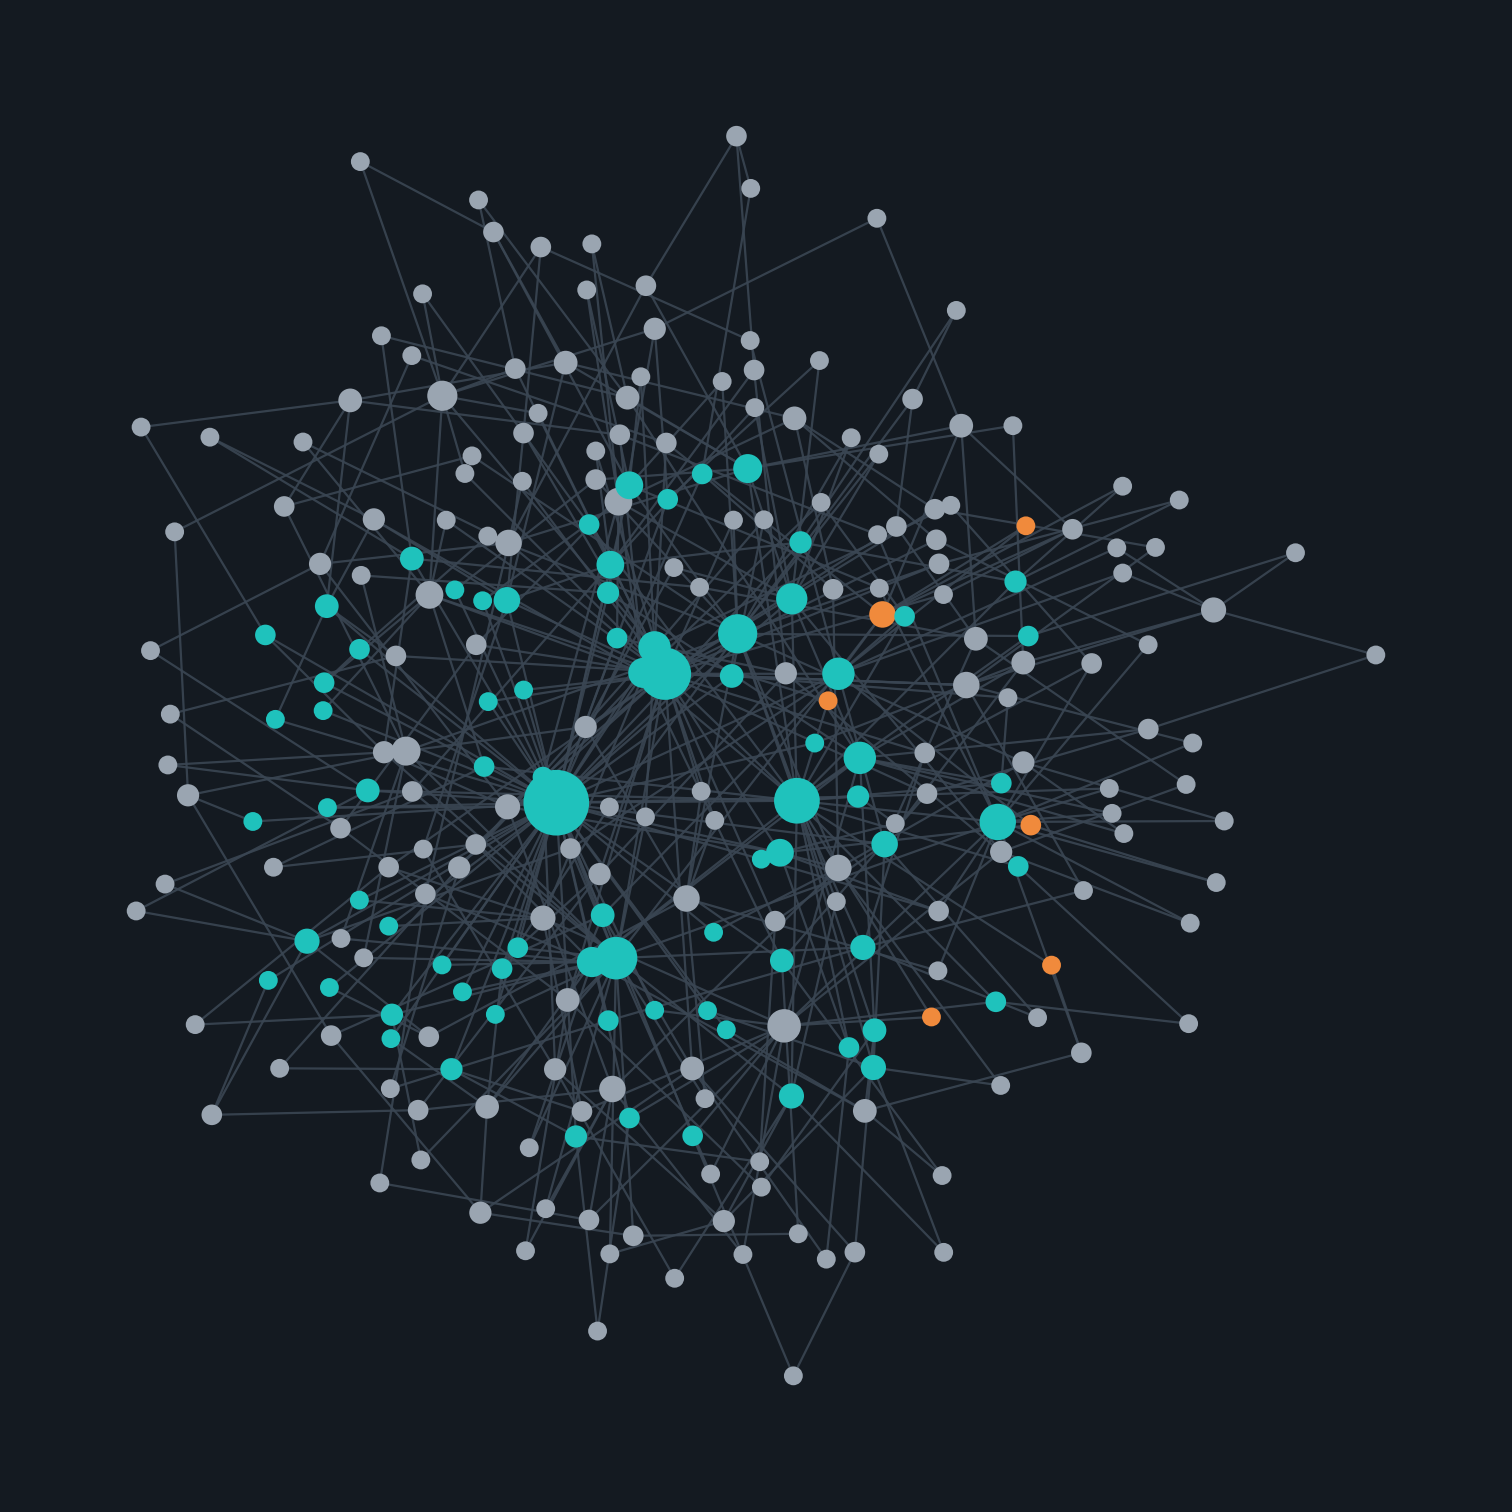
\includegraphics[width=\linewidth]{portada_red.png}
    \end{column}
  \end{columns}
\end{frame}
}
\note{\textbf{Jesus (0:40).} Buenos días. Somos Jesus, David y Duvan. Nuestro proyecto simula cómo se difunde un producto nuevo cuando cada persona decide influida por la publicidad y por sus contactos. Lo aplicamos a dos casos de actualidad: la PS5, una tecnología, y GTA\,6, un videojuego que sale este jueves. Lo construimos en NetLogo, lo calibramos con datos reales y lo usamos para comparar escenarios que no se pueden observar.}

% =================================================================== 2. motivación
\renewcommand{\seccion}{Motivación}
\begin{frame}{Dos lanzamientos, dos maneras de difundirse}
  \vskip4mm
  \begin{columns}[t,totalwidth=\textwidth]
    \begin{column}{0.31\textwidth}\cifra{\cifraPsUnidadesFin\,M}{PS5 vendidas de noviembre de 2020 a septiembre de 2026}\end{column}
    \begin{column}{0.31\textwidth}\cifra{19 nov.}{sale GTA\,6, solo para consolas de esta generación}\end{column}
    \begin{column}{0.31\textwidth}\cifra{90\,M}{vistas del primer tráiler de GTA\,6 en 24 horas}\end{column}
  \end{columns}
  \vskip8mm
  \begin{itemize}
    \item Bass: un producto se difunde por \textcolor{terracota}{publicidad} (externa) e \textcolor{azul}{imitación} (voz a voz).
    \item La PS5 crece por imitación; un gran estreno vende casi todo al salir.
  \end{itemize}
  \fuente{Sony Interactive Entertainment, Business Data \& Sales; Guinness World Records (2023).}
\end{frame}
\note{\textbf{Jesus (0:45).} La PS5 ya pasa de \cifraPsUnidadesFin\ millones de unidades, y sobre esa base sale GTA\,6 el 19 de noviembre, después de una campaña que rompió récords: 90 millones de vistas del primer tráiler en un día. Bass explicó la difusión con dos fuerzas: la publicidad, que llega a todos, y la imitación, que depende de cuántos ya adoptaron. Cuando manda la imitación sale la curva en S, como en la PS5; cuando manda la publicidad, las ventas se concentran en el lanzamiento.}

% =================================================================== 3. problema
\renewcommand{\seccion}{Problema}
\begin{frame}{El modelo agregado no ve la red social}
  \vskip2mm
  \begin{columns}[c,totalwidth=\textwidth]
    \begin{column}{0.52\textwidth}
      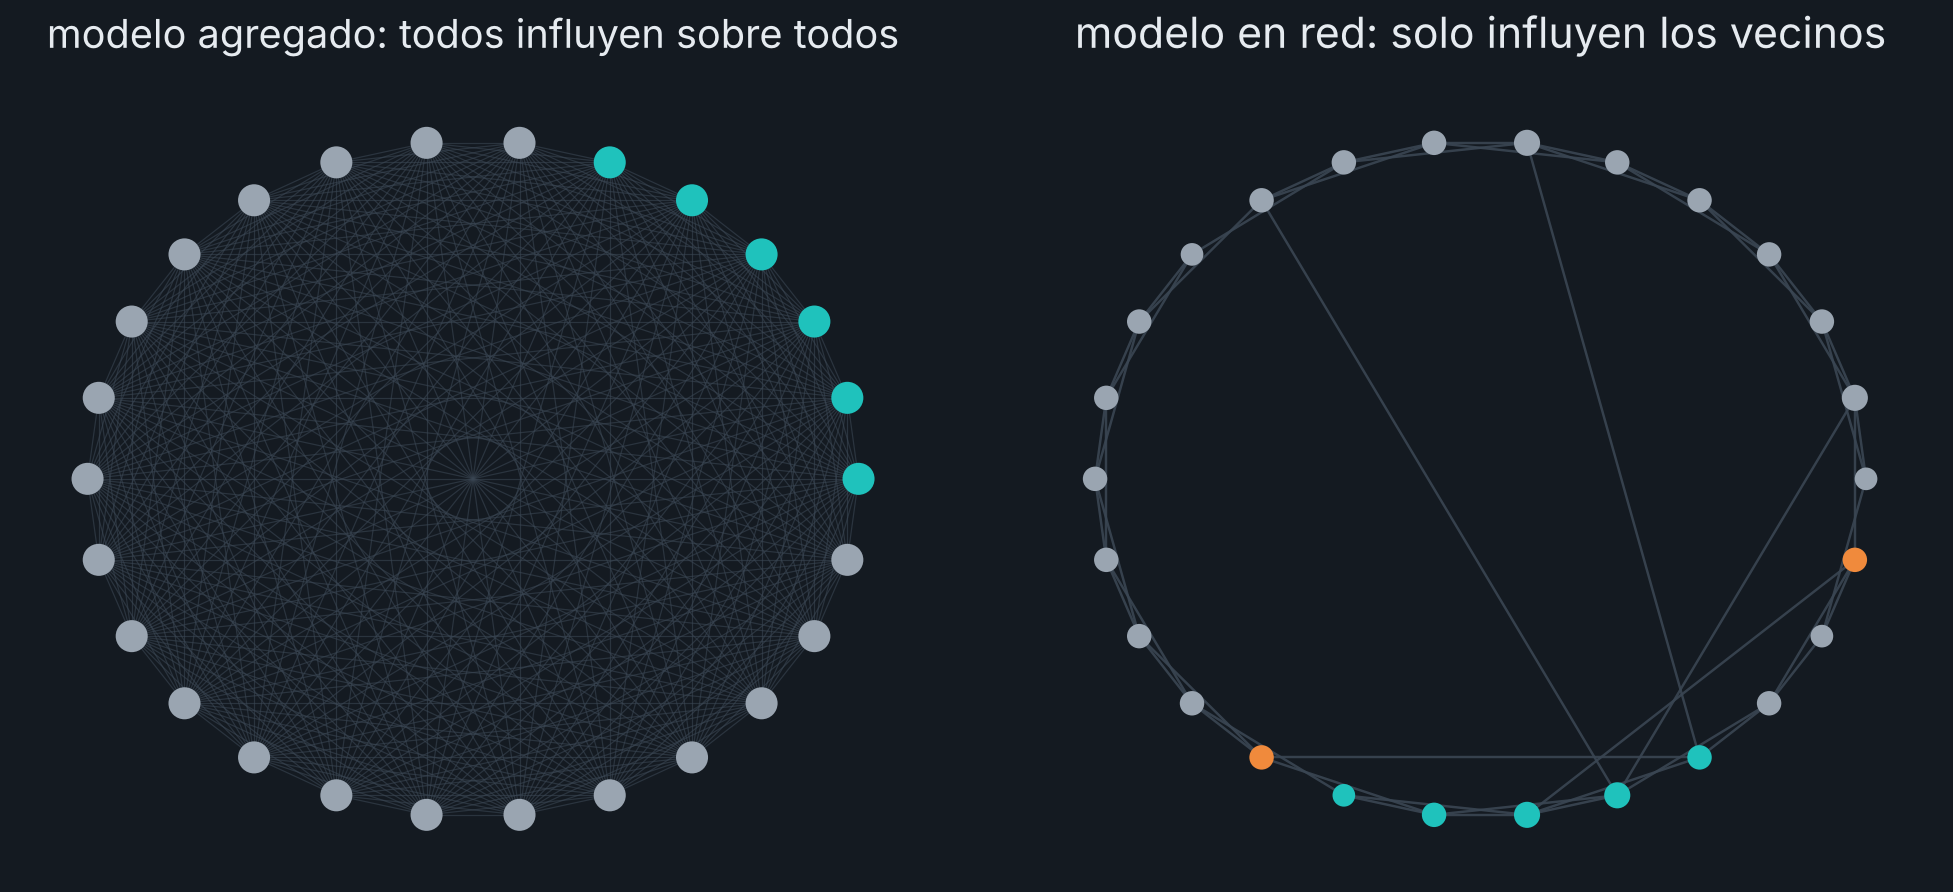
\includegraphics[width=\linewidth]{mezcla_vs_red.png}
    \end{column}
    \begin{column}{0.44\textwidth}
      \raggedright
      Bass: todos influyen sobre todos. En la realidad, solo los contactos.\par\vskip3mm
      \begin{itemize}
        \item ¿Qué pasa sin publicidad?
        \item ¿Importa la densidad o la forma de la red?
        \item ¿Cuánto se pierde con una campaña corta?
        \item ¿Responden igual una consola y un videojuego?
      \end{itemize}
    \end{column}
  \end{columns}
\end{frame}
\note{\textbf{Jesus (0:50).} El modelo de Bass describe bien las curvas agregadas, pero supone que todos influyen sobre todos, como en la red de la izquierda. En la vida real la influencia viaja por una red concreta, como la de la derecha. Eso deja cuatro preguntas sin responder: qué pasa sin publicidad, si importa la estructura de la red, cuánto se pierde con una campaña corta y si una consola y un videojuego responden igual.}

% =================================================================== 4. justificación
\renewcommand{\seccion}{Justificación}
\begin{frame}{Simular permite probar lo que no se puede observar}
  \vskip5mm
  \begin{columns}[t,totalwidth=\textwidth]
    \begin{column}{0.3\textwidth}
      {\plexmedia\color{azul}Individuos y red}\par\vskip2mm
      \nota{Cada persona es un agente con sus contactos y una regla de decisión.}
    \end{column}
    \begin{column}{0.3\textwidth}
      {\plexmedia\color{azul}Contrafactuales}\par\vskip2mm
      \nota{Lanzar sin publicidad, cambiar la red o acortar la campaña: imposible de observar en la realidad.}
    \end{column}
    \begin{column}{0.3\textwidth}
      {\plexmedia\color{azul}Datos reales}\par\vskip2mm
      \nota{PS5: calibrada y evaluada con ventas oficiales. GTA\,6, sin ventas aún: por analogía con GTA\,V.}
    \end{column}
  \end{columns}
  \vskip10mm
  \nota{NetLogo: libre, el modelo completo en un archivo y BehaviorSpace para repetir cada escenario 30 veces.}
\end{frame}
\note{\textbf{Jesus (0:50).} La simulación basada en agentes responde esas preguntas porque representa a cada persona y sus contactos, y permite correr escenarios que no se pueden observar, como lanzar sin publicidad. Para que no fuera un ejercicio solo cualitativo, la PS5 se calibró con las ventas oficiales de Sony y se evaluó con datos que no usamos para ajustar. GTA\,6 todavía no tiene ventas, así que sus parámetros salen por analogía con GTA\,V, que es la práctica estándar antes de un lanzamiento.}

% =================================================================== 5. objetivos
\renewcommand{\seccion}{Objetivos}
\begin{frame}{Qué nos propusimos}
  \vskip2mm
  {\plexmedia General.} Medir el efecto de la publicidad y de la red sobre la adopción final, en la PS5 y en GTA\,6.\par\vskip5mm
  {\plexmedia Específicos}\par\vskip1mm
  \begin{enumerate}
    \item Implementar en NetLogo el modelo de Bass en red, con tres tipos de red.
    \item Calibrar con la PS5 (entrenamiento, validación, prueba) y parametrizar GTA\,6 por analogía.
    \item Evaluar con 30 réplicas publicidad, densidad, topología y duración.
    \item Verificar con una reimplementación en Python.
  \end{enumerate}
\end{frame}
\note{\textbf{Jesus (0:40).} El objetivo general es medir el efecto de la publicidad y de la red sobre la adopción final, en la PS5 y en GTA\,6. Los específicos: implementarlo en NetLogo con tres tipos de red, calibrarlo con partición entrenamiento-validación-prueba, evaluar los escenarios con réplicas y verificarlo con una reimplementación independiente en Python.}

% =================================================================== 6. modelo
\renewcommand{\seccion}{Metodología}
\begin{frame}{Cada mes, cada persona decide: publicidad y vecinos}
  \vskip4mm
  \begin{center}{\Large $P_i = 1 - (1 - \textcolor{terracota}{p\,a_t})\,(1 - \textcolor{azul}{q\,f_i})$}\end{center}
  \vskip5mm
  \begin{columns}[T,totalwidth=\textwidth]
    \begin{column}{0.46\textwidth}
      {\color{terracota}\plexmedia publicidad}\par\nota{$p$: probabilidad mensual de que la campaña convenza; $a_t=1$ mientras está activa.}\par\vskip3mm
      {\color{azul}\plexmedia imitación}\par\nota{$q$ por $f_i$, la fracción de vecinos que ya adoptó.}
    \end{column}
    \begin{column}{0.48\textwidth}
      \vskip-\topsep
      {\small\begin{itemize}
        \item Adoptar es irreversible; todos deciden a la vez.
        \item Red completa = Bass: la diferencia es el efecto de la red.
        \item Redes aleatoria, mundo pequeño y libre de escala.
      \end{itemize}}
    \end{column}
  \end{columns}
\end{frame}
\note{\textbf{Jesus (1:00).} Cada agente es un nodo. Cada mes, quien no ha adoptado lo hace con esta probabilidad: la publicidad lo convence con probabilidad $p$ mientras la campaña esté activa, y sus vecinos con $q$ por la fracción de vecinos que ya adoptaron. Las decisiones se aplican todas a la vez al cerrar el mes y la adopción es irreversible. Si la red fuera completa, el modelo recuperaría la curva de Bass; la diferencia entre ambas es el efecto de la red. Usamos tres redes: aleatoria, mundo pequeño, con grupos cerrados, y libre de escala, con pocos nodos muy conectados. \emph{Le paso la palabra a David.}}

% =================================================================== 7. esquema
\begin{frame}{Del dato al escenario}
  \vskip2mm
  \begin{center}
  \begin{tikzpicture}[
    font=\small, text=tinta,
    caja/.style={draw=borde, line width=0.5pt, rounded corners=2pt, fill=white, align=center, inner sep=2pt,
                 minimum height=12mm, text width=21mm},
    etapa/.style={caja, fill=claro},
    flecha/.style={-{Latex[length=2mm]}, line width=0.8pt, draw=tinta},
    detalle/.style={font=\scriptsize, text=secundario}]
    \node[etapa] (d) at (0,0) {\plexmedia Datos\\[-1pt]{\scriptsize\color{secundario}Sony, Take-Two}};
    \node[etapa] (c) at (2.78,0) {\plexmedia Calibración\\[-1pt]{\scriptsize\color{secundario}Bass, analogía}};
    \node[etapa, fill=azulfondo, draw=azul, line width=0.8pt] (m) at (5.56,0) {\plexmedia Modelo\\[-1pt]{\scriptsize\color{secundario}NetLogo + nw}};
    \node[etapa] (e) at (8.34,0) {\plexmedia Escenarios\\[-1pt]{\scriptsize\color{secundario}BehaviorSpace}};
    \node[etapa] (a) at (11.12,0) {\plexmedia Análisis\\[-1pt]{\scriptsize\color{secundario}Python}};
    \draw[flecha] (d) -- (c); \draw[flecha] (c) -- (m);
    \draw[flecha] (m) -- (e); \draw[flecha] (e) -- (a);
    % interior del modelo
    \node[caja, fill=terracotafondo, draw=terracota, text width=27mm, minimum height=9mm] (camp) at (1.6,-2.5)
      {\plexmedia Campaña\\[-1pt]{\scriptsize $p\,a_t$}};
    \node[caja, fill=azulfondo, draw=azul, text width=27mm, minimum height=9mm] (red) at (1.6,-3.75)
      {\plexmedia Red social\\[-1pt]{\scriptsize $q\,f_i$}};
    \node[caja, fill=white, draw=azul, line width=0.8pt, text width=44mm, minimum height=21mm] (regla) at (6.3,-3.125)
      {\plexmedia Regla de adopción\\[4pt]$P_i = 1-(1-p\,a_t)(1-q\,f_i)$};
    \node[caja, text width=22mm, minimum height=12mm] (est) at (10.62,-3.125) {\plexmedia Estado\\[-1pt]{\scriptsize adopta y no vuelve atrás}};
    \draw[flecha, draw=terracota] (camp.east) -- (regla.west |- camp.east);
    \draw[flecha, draw=azul] (red.east) -- (regla.west |- red.east);
    \draw[flecha] (regla) -- (est);
    \begin{scope}[on background layer]
      \node[draw=azul, dashed, rounded corners=3pt, fit=(camp)(red)(regla)(est), inner sep=2.5mm] (int) {};
    \end{scope}
    \node[font=\scriptsize, text=azul, anchor=south west] at (int.north west) {cada mes, dentro del modelo};
    \draw[flecha, draw=azul, dashed] (m.south) -- (m.south |- int.north);
  \end{tikzpicture}
  \end{center}
\end{frame}
\note{\textbf{David (0:40).} Arriba el flujo: las ventas reales dan los parámetros, la PS5 por calibración de Bass y GTA\,6 por analogía con GTA\,V; NetLogo simula; BehaviorSpace corre los cuatro experimentos; Python calcula las medidas. Abajo, lo que pasa dentro del modelo cada mes: la campaña y la red alimentan la regla, que decide si cada persona adopta.}

% =================================================================== 8. implementación
\begin{frame}[fragile]{Implementación en NetLogo}
  \vskip1mm
  \begin{columns}[c,totalwidth=\textwidth]
    \begin{column}{0.47\textwidth}
      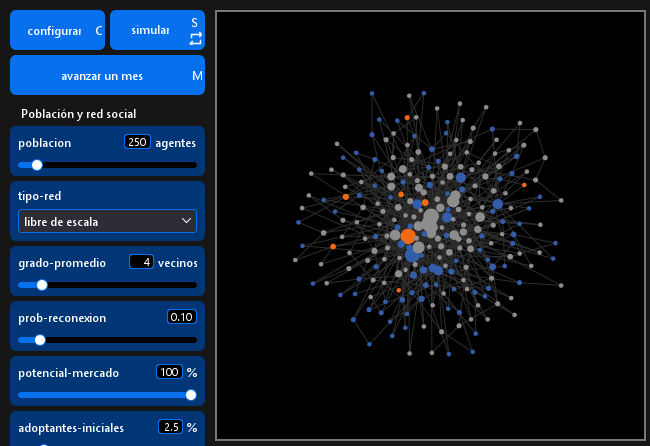
\includegraphics[width=\linewidth]{netlogo_ps5.png}\par\vskip1mm
      {\fontsize{6}{7}\selectfont\color{tenue}Interfaz del modelo (configuración de demostración: caso PS5, red libre de escala, mes 30).}
    \end{column}
    \begin{column}{0.5\textwidth}
\begin{lstlisting}
to decidir
  let p p-efectivo
  ask turtles with
      [susceptible? and not adoptante?] [
    let vecinos link-neighbors
    let f 0
    if any? vecinos [
      set f count vecinos with [adoptante?]
        / count vecinos ]
    let prob 1 - (1 - p) * (1 - q-imitacion * f)
    set decide-adoptar? random-float 1 < prob ]
end
\end{lstlisting}
      \vskip4mm
      \nota{\texttt{actualizar} aplica todas las decisiones a la vez. La extensión nw genera las redes; el selector de caso carga PS5, GTA\,6 o libre.}
    \end{column}
  \end{columns}
\end{frame}
\note{\textbf{David (0:50).} Esto es NetLogo con la extensión nw. A la izquierda, la interfaz con el caso PS5 en una red libre de escala: en azul los que ya adoptaron, en naranja los de este mes, y los nodos grandes son los más conectados. A la derecha, el procedimiento decidir: cada no adoptante cuenta qué fracción de sus vecinos ya adoptó y sortea su decisión con la fórmula. Un procedimiento aparte, actualizar, aplica todas las decisiones a la vez para que el orden de los agentes no afecte el resultado. El selector de caso carga los parámetros de la PS5 o de GTA\,6 con un clic.}

% =================================================================== 9. datos PS5
\renewcommand{\seccion}{Conjunto de datos}
\begin{frame}{La PS5: \cifraTrimestres\ trimestres de ventas oficiales de Sony}
  \begin{columns}[c,totalwidth=\textwidth]
    \begin{column}{0.6\textwidth}
      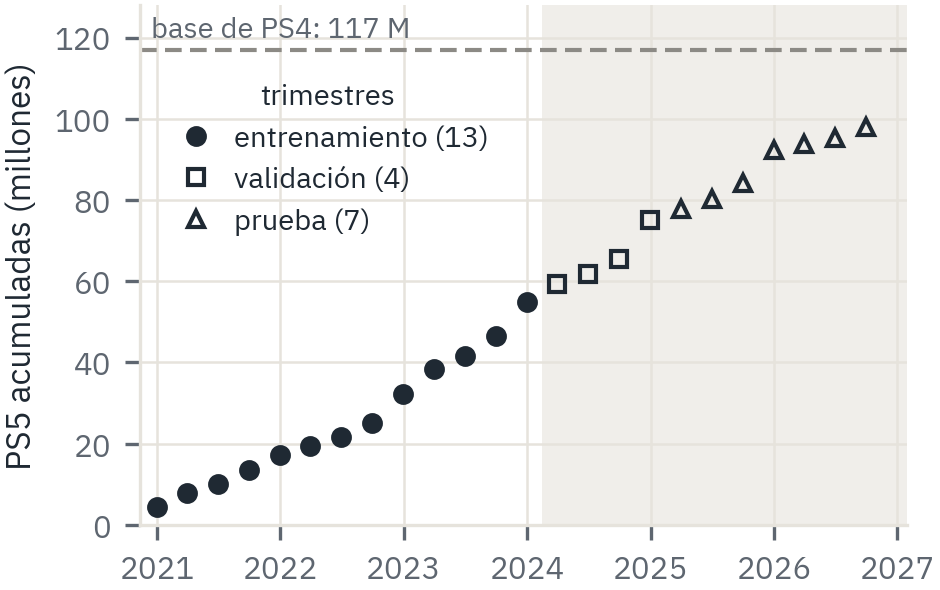
\includegraphics[width=\linewidth]{serie_ps5.png}
    \end{column}
    \begin{column}{0.36\textwidth}
      {\small\begin{itemize}
        \item \cifraPsUnidadesIni\ a \cifraPsUnidadesFin\ millones acumulados, dic.\,2020 a sep.\,2026.
        \item Adopción = acumulado / base de PS4 (\cifraUniverso\,M), fijada antes de ver la prueba.
        \item Simulación: \cifraCorridas\ corridas de 1000 agentes.
      \end{itemize}}
    \end{column}
  \end{columns}
  \fuente{Sony Interactive Entertainment, Business Data \& Sales (unidades vendidas a tiendas).}
\end{frame}
\note{\textbf{David (0:40).} La serie real son las unidades de PS5 que Sony publica cada trimestre: \cifraTrimestres\ trimestres, de \cifraPsUnidadesIni\ a \cifraPsUnidadesFin\ millones. La expresamos como porcentaje de la base de la PS4, \cifraUniverso\ millones, que fijamos antes de mirar los datos de prueba. El segundo conjunto lo genera la simulación: \cifraCorridas\ corridas de mil agentes.}

% =================================================================== 10. analogía GTA V
\begin{frame}{GTA\,6 aún no tiene ventas: lo parametrizamos con GTA\,V}
  \begin{columns}[c,totalwidth=\textwidth]
    \begin{column}{0.54\textwidth}
      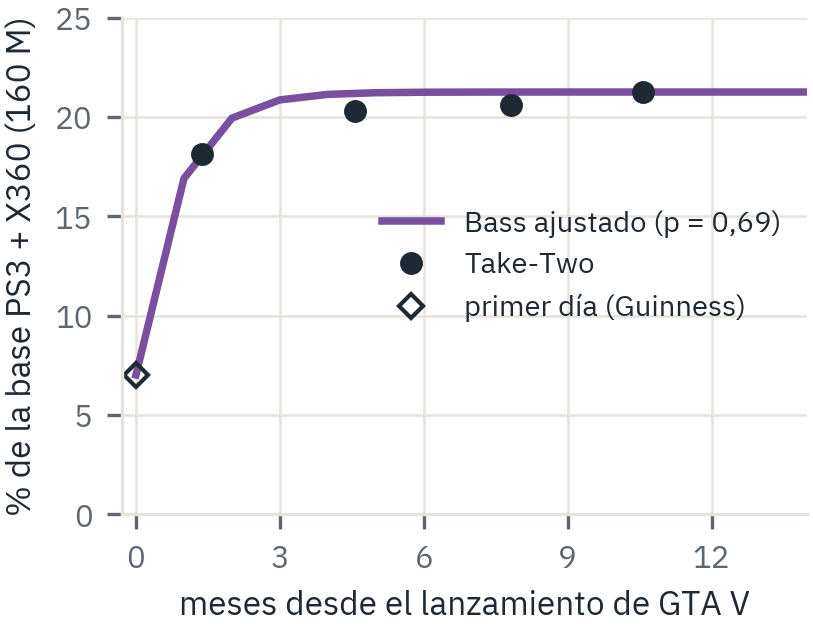
\includegraphics[width=0.94\linewidth]{analogia_gtav.png}
    \end{column}
    \begin{column}{0.42\textwidth}
      {\small\begin{itemize}
        \item GTA\,V: \cifraGtavSeisSemanas\,M en seis semanas y \cifraGtavMeseta\,M al año, sobre \cifraGtaBase\,M de consolas.
        \item Mismo ajuste de Bass: publicidad de \textcolor{terracota}{\cifraGtaP} al mes, unas \cifraGtaRazonPQ\ veces la imitación.
        \item GTA\,6 entre dueños de PS5: potencial \cifraGtaM\,\%, \cifraGtaIniciales\,\% el primer día, \cifraGtaHorizonte\ meses.
      \end{itemize}}
    \end{column}
  \end{columns}
  \fuente{Take-Two Interactive, resultados trimestrales 2013--2014; primer día: Guinness World Records (2013).}
\end{frame}
\note{\textbf{David (0:50).} GTA\,6 no tiene ventas todavía, así que usamos el método de analogía: tomamos el lanzamiento más parecido, GTA\,V. Vendió \cifraGtavSeisSemanas\ millones en seis semanas y se estabilizó en \cifraGtavMeseta\ millones, sobre \cifraGtaBase\ millones de consolas. Con la imitación fijada en la de la PS5, el ajuste atribuye el salto del lanzamiento a la publicidad: \cifraGtaP\ al mes, unas \cifraGtaRazonPQ\ veces la imitación, lo contrario de la PS5. Así modelamos GTA\,6 entre los dueños de PS5, con un potencial del \cifraGtaM\,\% y dos años de horizonte.}

% =================================================================== 11. diseño experimental
\renewcommand{\seccion}{Diseño experimental}
\begin{frame}{Cuatro experimentos, 30 réplicas por escenario}
  \vskip2mm
  \begin{tikzpicture}[x=1mm, y=1mm, font=\scriptsize]
    \fill[azul] (0,0) rectangle (60,10);
    \fill[azulclaro] (61,0) rectangle (92,10);
    \fill[terracota] (93,0) rectangle (134,10);
    \node[text=white, align=center] at (30,5) {entrenamiento\\dic.\,2020--dic.\,2023 · \cifraObsEnt\ trimestres};
    \node[text=tinta, align=center] at (76.5,5) {validación\\2024 · \cifraObsVal\ trimestres};
    \node[text=white, align=center] at (113.5,5) {prueba\\2025--2026 · \cifraObsPru\ trimestres};
    \node[text=secundario] at (30,-3) {ajusta $p$ y $q$};
    \node[text=secundario] at (76.5,-3) {elige $m$ y la red};
    \node[text=secundario] at (113.5,-3) {solo evalúa};
  \end{tikzpicture}
  \vskip6mm
  {\footnotesize
  \begin{tabular}{@{}lp{0.74\textwidth}r@{}}
    \toprule
    & factores (E1 a E3 para ambos casos: PS5 y GTA\,6) & corridas\\
    \midrule
    E1 & publicidad \{sin, con\} $\times$ densidad $k$ = 2, 4, 6, 8, 12, 16 & 720\\
    E2 & publicidad $\times$ topología \{aleatoria, mundo pequeño, libre de escala\} & 360\\
    E3 & duración de la campaña \{0, 1, 3, 6, 12, 24 meses, permanente\} & 420\\
    E4 & calibración PS5: 3 topologías $\times$ $k$ = 4, 8, 16 & 270\\
    \bottomrule
  \end{tabular}}
\end{frame}
\note{\textbf{David (0:50).} La serie de la PS5 se parte en el tiempo: con entrenamiento estimamos $p$ y $q$; como el potencial no se puede estimar en plena fase de crecimiento, lo elegimos en validación, igual que la red; la prueba solo evalúa. Corremos cuatro experimentos, los tres de escenarios para los dos casos: publicidad por densidad, publicidad por topología y duración de la campaña, más la calibración. Cada combinación se repite 30 veces. \emph{Duvan presenta las medidas y los resultados.}}

% =================================================================== 12. medidas
\renewcommand{\seccion}{Medidas de desempeño}
\begin{frame}{Cómo medimos}
  \vskip4mm
  \begin{columns}[T,totalwidth=\textwidth]
    \begin{column}{0.47\textwidth}
      {\plexmedia\color{azul}Escenarios}\par\vskip1mm
      {\small\begin{itemize}
        \item \alert{Adopción final}: \% de la población que adoptó al final del período (PS5: \cifraHorizontePs\ meses; GTA\,6: \cifraHorizonteGta).
        \item Mes del 50\,\% y mes del pico de compras.
        \item Media e IC del 95\,\% con 30 réplicas.
      \end{itemize}}
    \end{column}
    \begin{column}{0.47\textwidth}
      {\plexmedia\color{azul}Ajuste a la serie real}\par\vskip1mm
      {\small\begin{itemize}
        \item RMSE: raíz del error cuadrático medio, en puntos porcentuales.
        \item MAPE: error porcentual absoluto medio.
        \item Por partición: entrenamiento, validación y prueba.
      \end{itemize}}
    \end{column}
  \end{columns}
\end{frame}
\note{\textbf{Duvan (0:30).} La medida principal, la que pide el enunciado, es el porcentaje de adopción al final del período: seis años para la PS5 y dos para GTA\,6. La complementamos con el mes del 50\,\% y el mes del pico de compras. Frente a la serie real usamos RMSE y MAPE por partición. Todo con 30 réplicas e intervalos del 95\,\%.}

% =================================================================== 13. calibración
\renewcommand{\seccion}{Resultados}
\begin{frame}{El modelo sigue la serie de prueba de la PS5}
  \begin{columns}[c,totalwidth=\textwidth]
    \begin{column}{0.64\textwidth}
      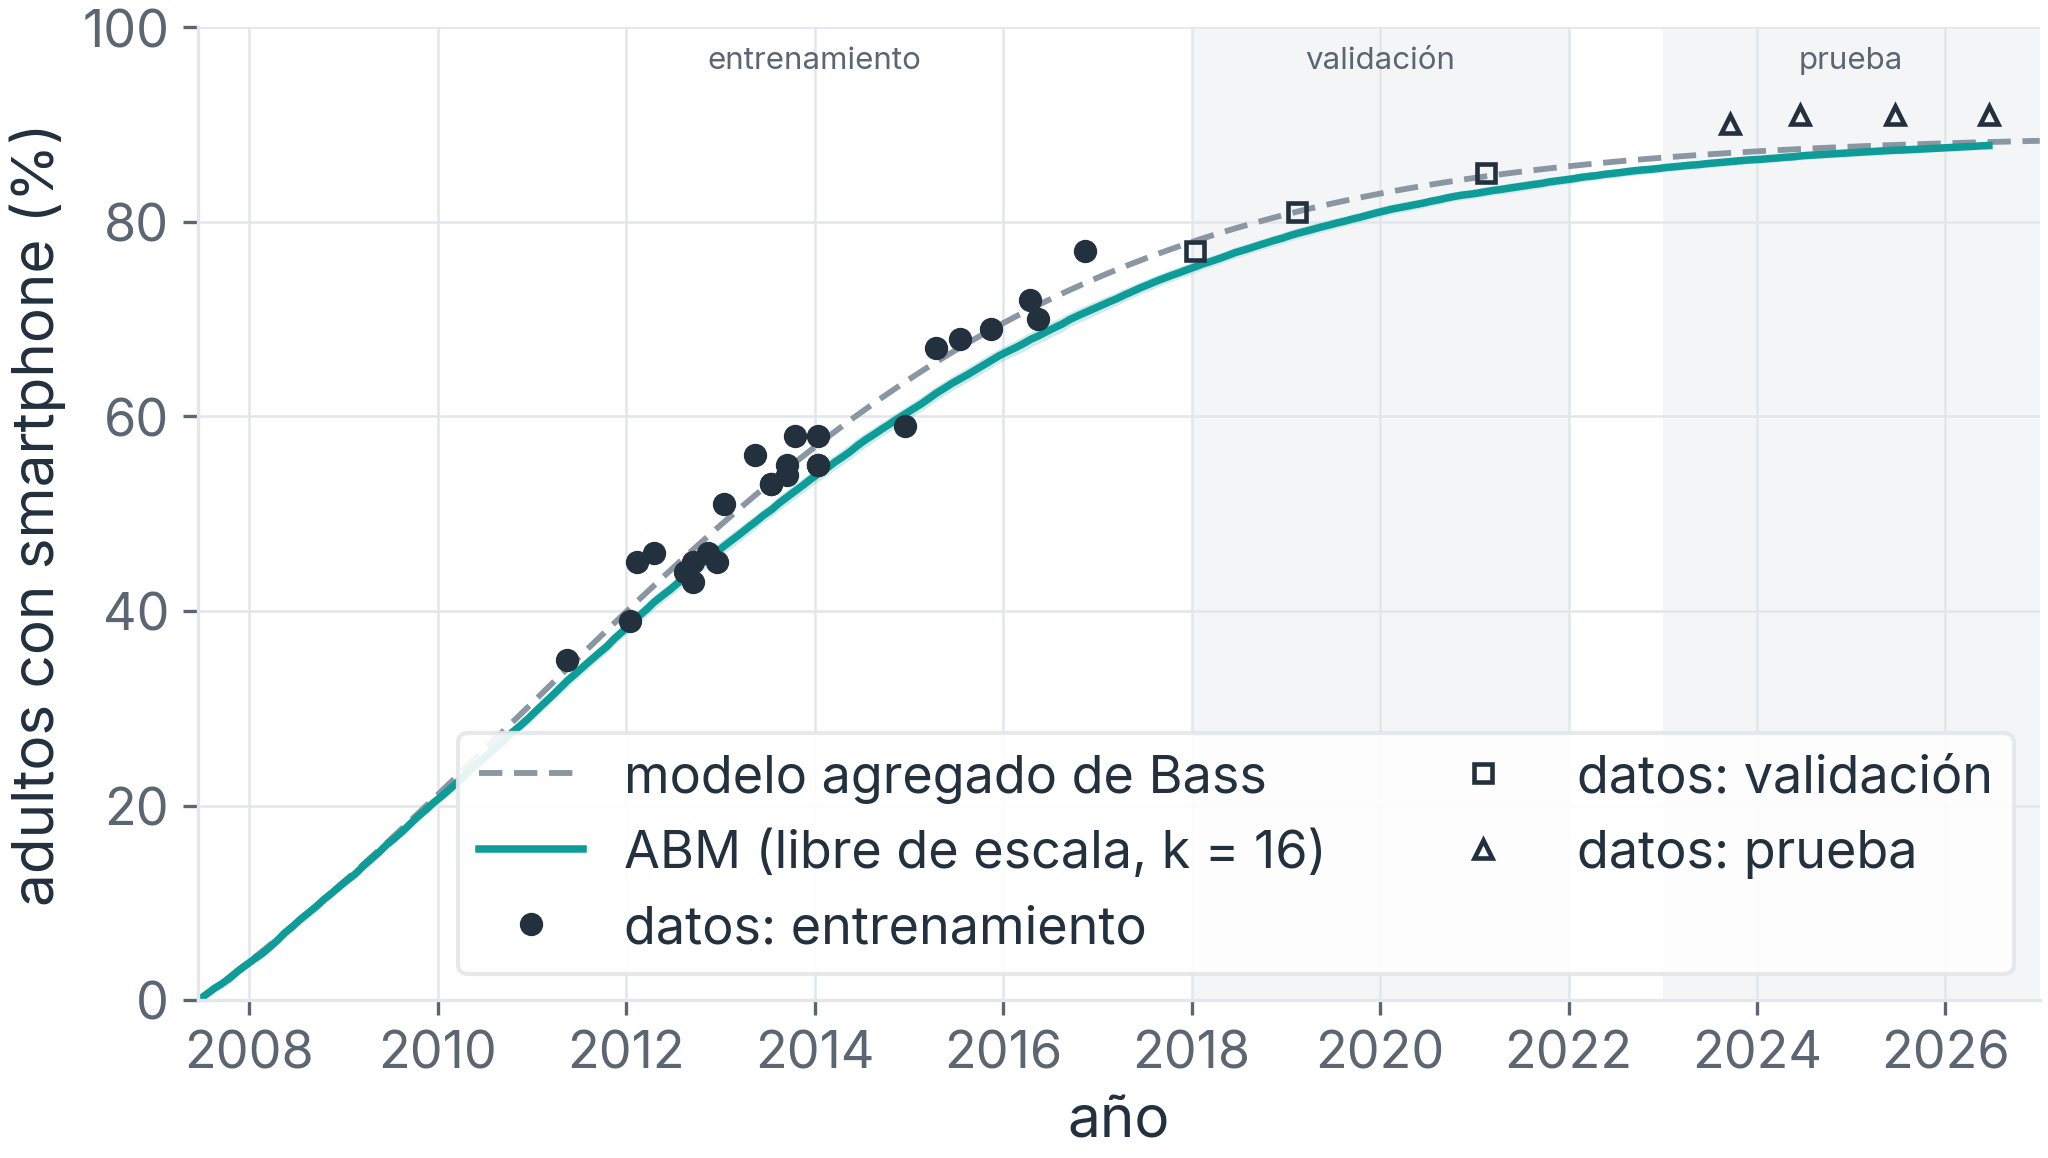
\includegraphics[width=\linewidth]{fig_calibracion.png}
    \end{column}
    \begin{column}{0.32\textwidth}
      \cifra{\cifraAbmRmsePru\ pp}{error en prueba del modelo de agentes (Bass: \cifraBassRmsePru)}\par\vskip5mm
      \nota{Bass anual: $p$\,=\,\cifraBassP, $q$\,=\,\cifraBassQ; la imitación pesa \cifraBassRazonQP\ veces más. Red elegida en validación: \cifraAbmSelRedNombre, $k$\,=\,\cifraAbmSelK.}
    \end{column}
  \end{columns}
\end{frame}
\note{\textbf{Duvan (0:50).} El ajuste da $p$ = \cifraBassP\ y $q$ = \cifraBassQ\ anuales: en la PS5 la imitación pesa \cifraBassRazonQP\ veces más que la publicidad. En validación se eligió la \cifraAbmSelRedNombre\ con $k$ = \cifraAbmSelK. En prueba, que nunca usamos para ajustar, el error es de \cifraAbmRmsePru\ puntos, mayor que el de Bass, \cifraBassRmsePru, porque la red frena la difusión. Ambos quedan un poco por debajo del dato de Sony de noviembre de 2026, más de 100 millones: la PS5 probablemente superará la base de la PS4.}

% =================================================================== 14. publicidad
\begin{frame}{Sin publicidad, ninguno de los dos llega lejos}
  \vskip1mm
  \begin{center}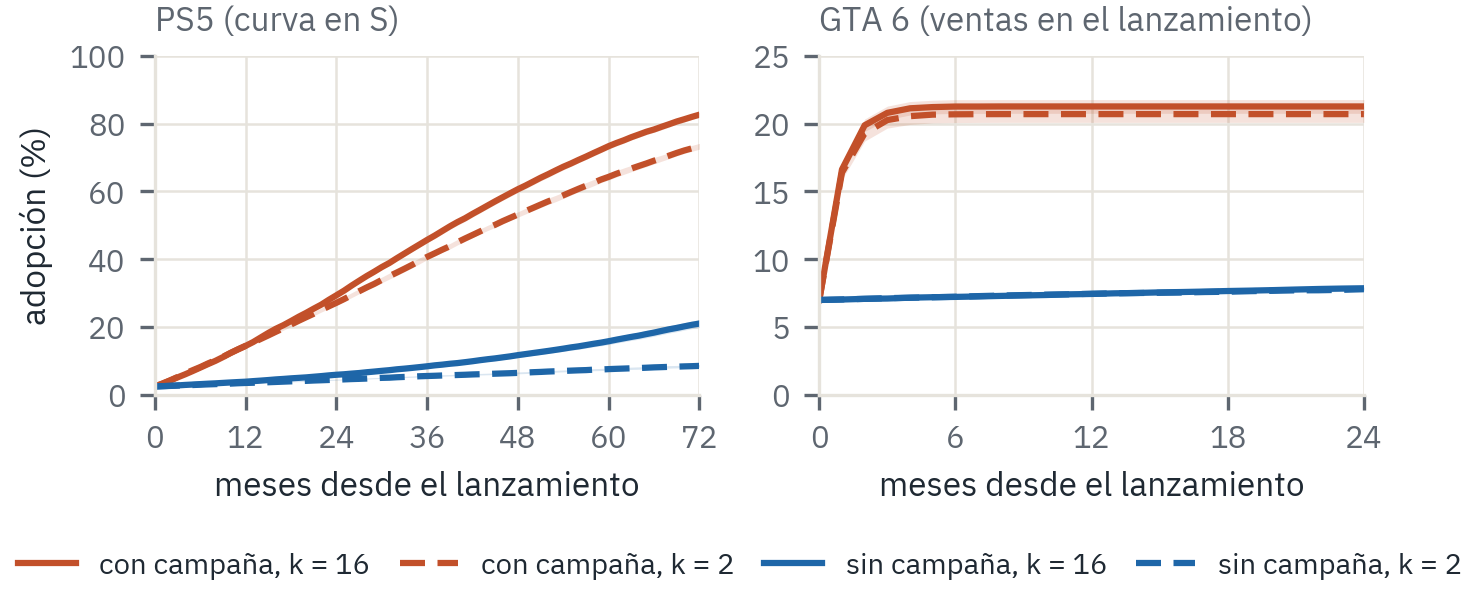
\includegraphics[width=0.9\linewidth]{publicidad_casos.png}\end{center}
  \vskip-3mm
  \nota{Red de mundo pequeño con $k$\,=\,2 (discontinua) y 16 (continua).}
\end{frame}
\note{\textbf{Duvan (0:50).} El resultado central. En la PS5, sin publicidad la adopción queda entre el \cifraPsSinMin\ y el \cifraPsSinMax\,\% en seis años; con campaña, entre el \cifraPsConMin\ y el \cifraPsConMax\,\%, con la curva en S. En GTA\,6 la campaña lo decide todo: con ella se alcanza el potencial casi en el primer mes; sin ella la adopción apenas pasa de los compradores del primer día. Sin publicidad, la PS5 simplemente no despega.}

% =================================================================== 15. densidad y topología
\begin{frame}{La red pesa sobre todo cuando no hay publicidad}
  \begin{columns}[c,totalwidth=\textwidth]
    \begin{column}{0.66\textwidth}
      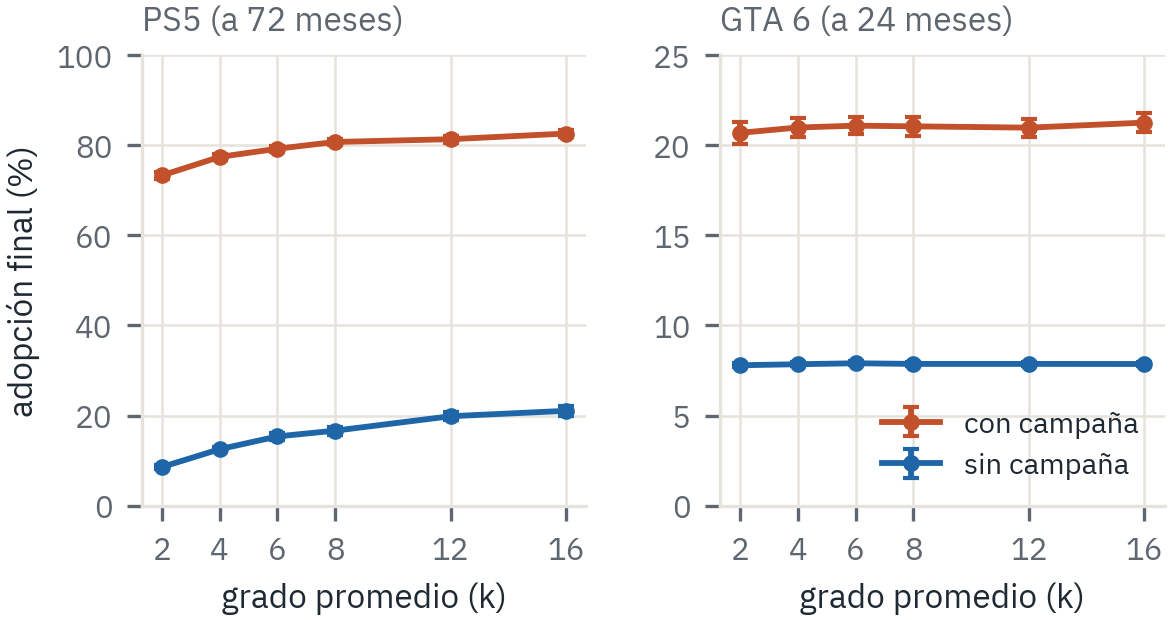
\includegraphics[width=\linewidth]{densidad.png}
    \end{column}
    \begin{column}{0.3\textwidth}
      \cifra{×\,\cifraPsSinRazon}{adopción de la PS5 sin campaña al pasar de $k$\,=\,2 a 16}\par\vskip4mm
      \nota{Con campaña, la misma diferencia solo la multiplica por \cifraPsConRazon. Sin campaña, la red de mundo pequeño es la topología más lenta.}
    \end{column}
  \end{columns}
\end{frame}
\note{\textbf{Duvan (0:50).} En la PS5 sin publicidad, pasar de 2 a 16 contactos multiplica la adopción por \cifraPsSinRazon; con campaña solo por \cifraPsConRazon, porque la publicidad siembra adoptantes en toda la red. En la topología pasa lo mismo: sin campaña, la red de mundo pequeño es la más lenta de las tres, porque sus grupos cerrados atrapan la influencia, y la libre de escala la más variable, porque depende de si un nodo muy conectado adopta temprano. En GTA\,6 la red casi no cambia nada.}

% =================================================================== 16. duración
\begin{frame}{GTA\,6: basta un mes; PS5: la campaña necesita tiempo}
  \begin{columns}[c,totalwidth=\textwidth]
    \begin{column}{0.58\textwidth}
      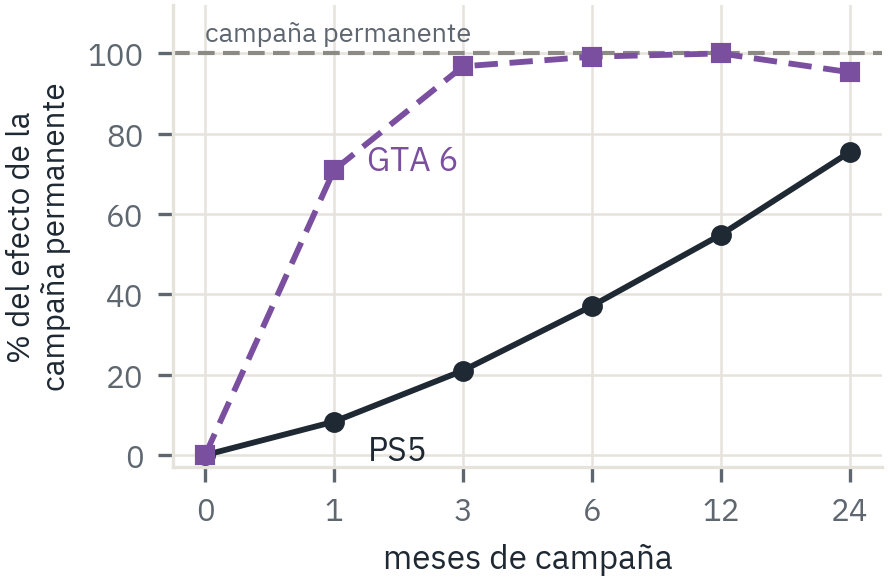
\includegraphics[width=\linewidth]{fraccion_duracion.png}
    \end{column}
    \begin{column}{0.38\textwidth}
      \cifra{\cifraFraccionGtaDUno\,\%}{del efecto de una campaña permanente se logra con un mes en GTA\,6}\par\vskip5mm
      \cifra{\cifraFraccionPsDDoce\,\%}{se logra con un año en la PS5 (dos años: \cifraFraccionPsDVeinticuatro\,\%)}
    \end{column}
  \end{columns}
\end{frame}
\note{\textbf{Duvan (0:40).} Si la campaña se corta, ¿cuánto se pierde? En GTA\,6, un solo mes ya logra el \cifraFraccionGtaDUno\,\% del efecto de una campaña permanente: el lanzamiento concentra casi todo. En la PS5 el rendimiento es gradual: un año logra el \cifraFraccionPsDDoce\,\% y dos años el \cifraFraccionPsDVeinticuatro\,\%, porque la imitación necesita tiempo para sostener la difusión. Los puntos de GTA\,6 que pasan apenas del 100\,\% son variación entre réplicas. \emph{David hace la demostración.}}

% =================================================================== 17. demo
\renewcommand{\seccion}{Demostración}
\begin{frame}{En vivo en NetLogo}
  \vskip1mm
  \begin{columns}[c,totalwidth=\textwidth]
    \begin{column}{0.4\textwidth}
      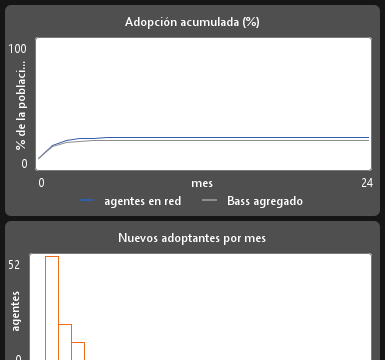
\includegraphics[width=0.86\linewidth]{netlogo_gta6.png}\par\vskip1mm
      {\fontsize{6}{7}\selectfont\color{tenue}Caso GTA\,6: compras concentradas en el primer mes.}
    \end{column}
    \begin{column}{0.56\textwidth}
      {\small\begin{enumerate}
        \item Caso \alert{GTA\,6} $\to$ configurar $\to$ simular: el pico llega en el primer mes.
        \item Campaña apagada: la adopción apenas pasa del \cifraGtaIniciales\,\%.
        \item Caso \textcolor{azul}{PS5}: curva en S frente a la de Bass.
      \end{enumerate}}
      \vskip2mm
      \nota{Si sobra tiempo: PS5 sin campaña y $k$ de 16 a 2; Herramientas $\to$ BehaviorSpace.}
    \end{column}
  \end{columns}
\end{frame}
\note{\textbf{David (1:10).} Demostración en vivo; los pasos están en el guion. Hacer 1 a 3; los otros dos solo si sobra tiempo.}

% =================================================================== 18. conclusiones
\renewcommand{\seccion}{Conclusiones}
\begin{frame}{Publicidad primero, red después}
  \vskip2mm
  \begin{enumerate}
    \item PS5: sin campaña, a lo sumo \cifraPsSinMaxGlobal\,\%; con campaña, al menos \cifraPsConMin\,\%.
    \item GTA\,6: un mes de campaña logra el \cifraFraccionGtaDUno\,\% del efecto.
    \item La red pesa sobre todo cuando no hay publicidad.
    \item Error en prueba: \cifraAbmRmsePru\ pp; la reimplementación en Python coincide.
  \end{enumerate}
  \vskip5mm
  \nota{Limitaciones: coeficientes iguales para todos, red fija, unidades vendidas a tiendas y parámetros de GTA\,6 hipotéticos.}
\end{frame}
\note{\textbf{Duvan (0:30).} Cuatro conclusiones. En la PS5, la publicidad es la condición del despegue. En GTA\,6, el primer mes de campaña decide el resultado. La red pesa sobre todo cuando no hay publicidad. Y el modelo quedó validado con datos que no usamos para ajustar y verificado con una reimplementación independiente.}

% =================================================================== 19. referencias
\renewcommand{\seccion}{Referencias}
\begin{frame}{Fuentes}
  \vskip0.5mm
  \raggedright\fontsize{8}{9.6}\selectfont
  \setlength{\parskip}{1.1mm}
  \referencia{Bass, F.\,M. (1969). A new product growth model for consumer durables. \textit{Management Science}, 15(5), 215--227.}
  \referencia{Goldenberg, J., Libai, B. y Muller, E. (2001). Talk of the network. \textit{Marketing Letters}, 12(3), 211--223.}
  \referencia{Rogers, E.\,M. (2003). \textit{Diffusion of Innovations} (5.ª ed.). Free Press.}
  \referencia{Thomas, R.\,J. (1985). Estimating market growth for new products: an analogical diffusion model approach. \textit{Journal of Product Innovation Management}, 2(1), 45--55.}
  \referencia{Watts, D.\,J. y Strogatz, S.\,H. (1998). Collective dynamics of `small-world' networks. \textit{Nature}, 393, 440--442.}
  \referencia{Wilensky, U. (1999). NetLogo. Northwestern University.}
  \referencia{Sony Interactive Entertainment (2026). Business Data \& Sales.}
  \referencia{Take-Two Interactive (2013--2014). Resultados trimestrales, años fiscales 2014 y 2015.}
  \referencia{Guinness World Records (2013, 2023). Récords de ventas de GTA\,V y de vistas del tráiler de GTA\,6.}
\end{frame}
\note{\textbf{Duvan (0:10).} Las referencias están en pantalla. Gracias; quedamos atentos a sus preguntas.}

\end{document}
